\RequirePackage{pdfmanagement-testphase}
\DeclareDocumentMetadata {lang=en-US}

% xmp metadata for pdf
% Originally used \usepackage[a-2a]{pdfx}
% \usepackage{hyperxmp} replaced it
% \RequirePackage{pdfmanagement-testphase} replaced it
% \PassOptionsToPackage{enable-debug,check-declarations}{expl3} broke with version 0.9 of tagpdf
% \ExplSyntaxOn no need for these 3 lines because metadata can handle it
% \pdfmanagement_add:nnn{Catalog}{Lang}{(enUS)} enUS is wrong, should be en-US
% \ExplSyntaxOff

\documentclass[11pt,
  english,
  a4paper,
]{article}
\usepackage{sa4ss}
\usepackage{amsmath,amssymb,array}
\usepackage{booktabs}

% From tagged-template.latex
\usepackage{lmodern}
\usepackage{ifxetex,ifluatex}
\ifnum 0\ifxetex 1\fi\ifluatex 1\fi=0 % if pdftex
  \usepackage[T1]{fontenc}
  \usepackage[utf8]{inputenc}
  \usepackage{textcomp} % provide euro and other symbols
\else % if luatex or xetex
  \usepackage{unicode-math}
  \defaultfontfeatures{Scale=MatchLowercase}
  \defaultfontfeatures[\rmfamily]{Ligatures=TeX,Scale=1}
\fi

% Use upquote if available, for straight quotes in verbatim environments
\IfFileExists{upquote.sty}{\usepackage{upquote}}{}
\IfFileExists{microtype.sty}{% use microtype if available
  \usepackage[]{microtype}
  \UseMicrotypeSet[protrusion]{basicmath} % disable protrusion for tt fonts
}{}
\makeatletter
\@ifundefined{KOMAClassName}{% if non-KOMA class
  \IfFileExists{parskip.sty}{%
    \usepackage{parskip}
  }{% else
    \setlength{\parindent}{0pt}
    \setlength{\parskip}{6pt plus 2pt minus 1pt}}
}{% if KOMA class
  \KOMAoptions{parskip=half}}
\makeatother
\usepackage{xcolor}
\IfFileExists{xurl.sty}{\usepackage{xurl}}{} % add URL line breaks if available
\hypersetup{
  pdftitle={The status of copper rockfish (Sebastes caurinus) in U.S. waters off the coast of California north of Point Conception in 2021 using catch and length data},
  pdflang={en},
  hidelinks,
  pdfcreator={LaTeX via pandoc}}
\urlstyle{same} % disable monospaced font for URLs
\usepackage{longtable}
% Correct order of tables after \paragraph or \subparagraph
\usepackage{etoolbox}
\makeatletter
\patchcmd\longtable{\par}{\if@noskipsec\mbox{}\fi\par}{}{}
\makeatother
% Allow footnotes in longtable head/foot
\IfFileExists{footnotehyper.sty}{\usepackage{footnotehyper}}{\usepackage{footnote}}
\makesavenoteenv{longtable}
\usepackage{graphicx}
\makeatletter
\def\maxwidth{\ifdim\Gin@nat@width>\linewidth\linewidth\else\Gin@nat@width\fi}
\def\maxheight{\ifdim\Gin@nat@height>\textheight\textheight\else\Gin@nat@height\fi}
\makeatother
% Scale images if necessary, so that they will not overflow the page
% margins by default, and it is still possible to overwrite the defaults
% using explicit options in \includegraphics[width, height, ...]{}
\setkeys{Gin}{width=\maxwidth,height=\maxheight,keepaspectratio}
% Set default figure placement to htbp
\makeatletter
\def\fps@figure{htbp}
\makeatother
\setlength{\emergencystretch}{3em} % prevent overfull lines
\providecommand{\tightlist}{%
  \setlength{\itemsep}{0pt}\setlength{\parskip}{0pt}}
\setcounter{secnumdepth}{5}
\ifxetex
  % Load polyglossia as late as possible: uses bidi with RTL langages (e.g. Hebrew, Arabic)
  \usepackage{polyglossia}
  \setmainlanguage[]{english}
\else
  \usepackage[shorthands=off,main=english]{babel}
\fi

\providecommand{\tightlist}{%
  \setlength{\itemsep}{0pt}\setlength{\parskip}{0pt}}


\date{}
\newcommand{\trTitle}{The status of copper rockfish (\emph{Sebastes caurinus}) in U.S. waters off the coast of California north of Point Conception in 2021 using catch and length data}
\newcommand{\trYear}{2021}
\newcommand{\trMonth}{May}
\newcommand{\trAuthsLong}{truetruetruetrue}
\newcommand{\trAuthsBack}{Wetzel, C.R., B.J. Langseth, J.M. Cope, J.E. Budrick}
\newcommand{\trCitation}{
\begin{hangparas}{1em}{1}
\trAuthsBack{}. \trYear{}. \trTitle{}. Pacific Fisheries Management Council, Portland, Oregon. \pageref{LastPage}{}\,p.
\end{hangparas}}

\AtBeginDocument{\tagstructbegin{tag=Document}}
\AtEndDocument{\tagstructend}
\pretocmd{\maketitle}{\tagstructbegin{tag=H1}\tagmcbegin{tag=H1}}{}{}
\apptocmd{\maketitle}{\tagmcend\tagstructend}{}{}

\begin{document}

%%%%% Frontmatter %%%%%

% Footnote symbols in front matter
\renewcommand*{\thefootnote}{\fnsymbol{footnote}}

\small
\thispagestyle{empty}
\pagenumbering{roman}
\noindent
\begin{center}
\title{The status of copper rockfish (\emph{Sebastes caurinus}) in U.S. waters off the coast of California north of Point Conception in 2021 using catch and length data}
% \textnormal{\MakeTextUppercase{\trTitle{}}}
\vspace{1.5cm}
{\Large\textbf\newline{The status of copper rockfish (\emph{Sebastes caurinus}) in U.S. waters off the coast of California north of Point Conception in 2021 using catch and length data}}
\vfill
by\\
Chantel R. Wetzel\textsuperscript{1}\\
Brian J. Langseth\textsuperscript{1}\\
Jason M. Cope\textsuperscript{1}\\
John E. Budrick\textsuperscript{2}\vfill
\textsuperscript{1}Northwest Fisheries Science Center, U.S. Department of Commerce, National Oceanic and Atmospheric Administration, National Marine Fisheries Service, 2725 Montlake Boulevard East, Seattle, Washington 98112\\
\textsuperscript{2}California Department of Fish and Wildlife, 350 Harbor Boulevard, Belmont, California 94002\vfill
\trMonth{} \trYear{}
\end{center}
\clearpage

% Fourth page: Colophon
\thispagestyle{empty}
\vspace*{\fill}
\begin{center}
\copyright{} Pacific Fisheries Management Council, \trYear{}\\
\end{center}
\par
\bigskip
\noindent
Correct citation for this publication:
\bigskip
\par
\trCitation{}
\clearpage

% Add TOC to pdf bookmarks (clickable pdf)
\pdfbookmark[1]{\contentsname}{toc}

% Table of contents page, lists of figures and tables
\tableofcontents\clearpage
%\listoffigures \listoftables \clearpage
\label{TRlastRoman}
\clearpage

% Table of contents
\newpage
\thispagestyle{empty} % to remove page number

% Settings for the main document
\pagenumbering{arabic}  % Regular page numbers
\pagestyle{plain}  % No page number on first page of main document, use 'empty'
\renewcommand*{\thefootnote}{\arabic{footnote}}  % Back to numeric footnotes
\setcounter{footnote}{0}  % And start at 1
\renewcommand{\headrulewidth}{0.5pt}
\renewcommand{\footrulewidth}{0.5pt}
%\pagestyle{fancy}\fancyhead[c]{Draft: Do not cite or circulate}

\newcommand{\lt}{\ensuremath <}
\newcommand{\gt}{\ensuremath >}

%Define cslreferences environment, required by pandoc 2.8
%https://github.com/rstudio/rmarkdown/issues/1649
\newlength{\cslhangindent}
\setlength{\cslhangindent}{1.5em}
\newenvironment{cslreferences}%
  {\setlength{\parindent}{0pt}%
  \everypar{\setlength{\hangindent}{\cslhangindent}}\ignorespaces}%
  {\par}

\pagenumbering{roman}
\setcounter{page}{1}

\renewcommand{\thetable}{\roman{table}}
\renewcommand{\thefigure}{\roman{figure}}

\setlength\parskip{0.5em plus 0.1em minus 0.2em}

\vspace{500cm}

\tagstructbegin{tag=H1}\tagmcbegin{tag=H1}

\hypertarget{disclaimer}{%
\section*{Disclaimer}\label{disclaimer}}
\addcontentsline{toc}{section}{Disclaimer}

\leavevmode\tagmcend\tagstructend

\tagstructbegin{tag=P}\tagmcbegin{tag=P}

\emph{\textbf{These materials do not constitute a formal publication and are for information only. They are in a pre-review, pre-decisional state and should not be formally cited or reproduced. They are to be considered provisional and do not represent any determination or policy of NOAA or the Department of Commerce.}}

\leavevmode\tagmcend\tagstructend\par

\pagebreak

\pagebreak
\setlength{\parskip}{5mm plus1mm minus1mm}
\pagenumbering{arabic}
\setcounter{page}{1}
\renewcommand{\thefigure}{\arabic{figure}}
\renewcommand{\thetable}{\arabic{table}}

\setcounter{table}{0}
\setcounter{figure}{0}

\setlength\parskip{0.5em plus 0.1em minus 0.2em}

\tagstructbegin{tag=H1}\tagmcbegin{tag=H1}

\hypertarget{introduction}{%
\section{Introduction}\label{introduction}}

\leavevmode\tagmcend\tagstructend

\tagstructbegin{tag=H2}\tagmcbegin{tag=H2}

\hypertarget{basic-information}{%
\subsection{Basic Information}\label{basic-information}}

\leavevmode\tagmcend\tagstructend

\tagstructbegin{tag=P}\tagmcbegin{tag=P}

This assessment reports the status of copper rockfish (\emph{Sebastes caurinus}) off the California coast, north of Point Conception, using data through 2020.

\leavevmode\tagmcend\tagstructend\par

\tagstructbegin{tag=P}\tagmcbegin{tag=P}

Copper rockfish is a medium- to large-sized nearshore rockfish found from Mexico to Alaska. The core range is comparatively large, from northern Baja Mexico to the Gulf of Alaska, as well as in Puget Sound. Copper rockfish have historically been a part of both commercial and recreational fisheries throughout its range.

\leavevmode\tagmcend\tagstructend\par

\tagstructbegin{tag=P}\tagmcbegin{tag=P}

Copper rockfish are commonly found in waters less than 130 meters in depth in nearshore kelp forests and rocky habitat {\tagstructbegin{tag=Reference}\tagmcbegin{tag=Reference}(Love 1996)\leavevmode\tagmcend\tagstructend}. The diets of copper rockfish consist primarily of crustaceans, mollusks, and fish {\tagstructbegin{tag=Reference}\tagmcbegin{tag=Reference}(Lea, McAllister, and VenTresca 1999; Bizzarro, Yoklavich, and Wakefield 2017)\leavevmode\tagmcend\tagstructend}. The body coloring of copper rockfish varies across the coast with northern fish often exhibiting dark brown to olive with southern fish exhibiting yellow to olive-pink variations in color {\tagstructbegin{tag=Reference}\tagmcbegin{tag=Reference}(Miller and Lea 1972)\leavevmode\tagmcend\tagstructend} which initially led to them being designated as two separate species (\emph{S. caurinus} and \emph{S. vexillaris}).

\leavevmode\tagmcend\tagstructend\par

\tagstructbegin{tag=P}\tagmcbegin{tag=P}

Numerous genetic studies have been performed looking for genetic variation in copper rockfish with variable outcomes. Genetic work has revealed significant differences between Puget Sound and coastal stocks {\tagstructbegin{tag=Reference}\tagmcbegin{tag=Reference}(Dick, Shurin, and Taylor 2014)\leavevmode\tagmcend\tagstructend}. Stocks along the West Coast have not been determined to be genetically distinct populations but significant population subdivision has been detected, indicating limited oceanographic exchange among geographically proximate locations {\tagstructbegin{tag=Reference}\tagmcbegin{tag=Reference}(Buonaccorsi et al. 2002; Johansson et al. 2008)\leavevmode\tagmcend\tagstructend}. A specific study examining copper rockfish populations off the coast of Santa Barbara and Monterey California identified a genetic break between the north and south with moderate differentiation {\tagstructbegin{tag=Reference}\tagmcbegin{tag=Reference}(Sivasundar and Palumbi 2010)\leavevmode\tagmcend\tagstructend}.

\leavevmode\tagmcend\tagstructend\par

\tagstructbegin{tag=P}\tagmcbegin{tag=P}

Copper rockfish are a relatively long-lived rockfish estimated to live at least 50 years {\tagstructbegin{tag=Reference}\tagmcbegin{tag=Reference}(Love 1996)\leavevmode\tagmcend\tagstructend}. Copper rockfish was determined to have the highest vulnerability (V = 2.27) of any West Coast groundfish stock evaluated in a productivity susceptibility analysis {\tagstructbegin{tag=Reference}\tagmcbegin{tag=Reference}(Cope et al. 2011)\leavevmode\tagmcend\tagstructend}. This analysis calculated species-specific vulnerability scores based on two dimensions: productivity characterized by the life history and susceptibility that characterized how the stock could be impacted by fisheries and other activities.

\leavevmode\tagmcend\tagstructend\par

\tagstructbegin{tag=H2}\tagmcbegin{tag=H2}

\hypertarget{historical-and-current-fishery-information}{%
\subsection{Historical and Current Fishery Information}\label{historical-and-current-fishery-information}}

\leavevmode\tagmcend\tagstructend

\tagstructbegin{tag=P}\tagmcbegin{tag=P}

Off the coast of California, north of Point Conception, copper rockfish is caught in both commercial and recreational fisheries. Recreational removals have been the largest source of fishing mortality, comprising nearly 85 percent of total removals of copper rockfish across all years (Table \ref{tab:allcatches} and Figure \ref{fig:catch}). The landings from the commercial fishery have been minimal by year, expect for a brief period between the mid-1980s and early-2000s.

\leavevmode\tagmcend\tagstructend\par

\tagstructbegin{tag=P}\tagmcbegin{tag=P}

The recreational fishery in the early part of the 20th century were focused on nearshore waters near ports, with activity expanded activity further from port and into deeper depths over time {\tagstructbegin{tag=Reference}\tagmcbegin{tag=Reference}(Miller et al. 2014)\leavevmode\tagmcend\tagstructend}. Prior to the groundfish fishery being declared a federal disaster 2000, and the subsequent rebuilding period, there were no time or area closures for groundfish. Access to deeper depths during this period spread effort over a larger area and filled bag limits with a greater diversity of species from both the shelf and nearshore. This resulted in lower catch of nearshore rockfish relative to the period after 2000 when 20 to 60 fm depth restrictions ranging from 20 fm in the Northern Management Area to 60 fm in the Southern Management Area were put in place in various management area delineations along the state (see Appendix Section \ref{ca-man}). This shifting effort onto the nearshore, concomitantly increased catch rates for nearshore rockfish including copper rockfish in the remaining open depths, though season lengths were greatly curtailed.

\leavevmode\tagmcend\tagstructend\par

\tagstructbegin{tag=P}\tagmcbegin{tag=P}

Following all previously overfished groundfish species, other than yelloweye rockfish, being declared rebuilt by 2019, deeper depth restrictions were offered in the Southern Management area allowing resumed access to shelf rockfish in less than 75 fm and are currently 100 fm as of 2021. The increased access to deeper depths south of Point Conception with the rebuilding of cowcod is expected to reduce the effort in nearshore waters where copper rockfish is most prevalent. To the north of Point Conception where yelloweye rockfish are prevalent, depth constraints persist and effort remains focused on the nearshore in 30 to 50 fm depending on the management area. As yelloweye rockfish continues to rebuild, incremental increases in access to deeper depths are expected, which will likely further reduce the effort in nearshore waters where copper rockfish is most prevalent.

\leavevmode\tagmcend\tagstructend\par

\tagstructbegin{tag=P}\tagmcbegin{tag=P}

Prior to development of the live fish market in the 1980s, there was very little commercial catch of copper rockfish, with dead copper rockfish fetching a low ex-vessel price per pound. Copper rockfish were targeted along with other rockfish to some degree in the nearshore or caught as incidental catch by vessels targeting other more valuable stocks such as lingcod. Most fish were caught using hook and line gear, though some were caught using traps, gill nets and, rarely, trawl gear. Trawling was prohibited within three miles of shore in 1953 and gill netting within three miles of shore was prohibited in 1994, preventing access to a high proportion of the species habitat with these gear types. Copper rockfish were targeted along with other rockfish to some degree in the nearshore or and caught as bycatch by vessels targeting other more valuable stocks such as lingcod.

\leavevmode\tagmcend\tagstructend\par

\tagstructbegin{tag=P}\tagmcbegin{tag=P}

In the late 1980s and early 1990s a market for fish landed live arose out of Los Angeles and the Bay area, driven by demand from Asian restaurants and markets. The growth of the live fish market was driven by consumers willing to pay a higher price for live fish, ideally plate-sized (12 - 14 inches or 30.5 - 35.6 cm). Live fish landed for the restaurant market lump fish into two categories, small (1 - 3 lbs.) or large (3 - 6 lbs.), with small, plate-sized, fish fetching higher prices at market ranging between \$5 -7 per fish (Bill James, personal communication). Copper rockfish is one of the many rockfish species that is included in the commercial live fish fishery. The proportion of copper rockfish being landed live vs.~dead since 2000 by California commercial fleets ranges between 50 to greater than 70 percent in the southern and northern areas, respectively.

\leavevmode\tagmcend\tagstructend\par

\tagstructbegin{tag=P}\tagmcbegin{tag=P}

With the development and expansion of the nearshore live fish fishery during the 1980s and 1990s, new entrants in this open access fishery were drawn by premium ex-vessel price per pound for live fish resulting in over-capitalization of the fishery. Since 2002, the California Department of Fish and Wildlife (CDFW) has managed 19 nearshore species in accordance with Nearshore Fisheries Management Plan {\tagstructbegin{tag=Reference}\tagmcbegin{tag=Reference}(Wilson-Vandenberg, Larinto, and Key 2014)\leavevmode\tagmcend\tagstructend}. In 2003, the CDFW implemented a Nearshore Restricted Access Permit system, including requirement of a Deeper Nearshore Fishery Species Permit to retain copper rockfish, with the overall goal of reducing the number of participants to a more sustainable level, with permit issuance based on historical landings history by the retrospective qualifying date. The result was reduction in permits issued from 1,127 in 1999 to 505 in 2003, greatly reducing catch levels. In addition, reduced trip limits, season closures in March and April and depth restrictions were implemented to address bycatch of overfished species and associated constraints from their low catch limits.

\leavevmode\tagmcend\tagstructend\par

\tagstructbegin{tag=P}\tagmcbegin{tag=P}

Copper rockfish residing between Point Conception and the California/Oregon border are assessed here as a single, separate stock. This designation was made based on oceanographic, geographic, and fishery conditions. The copper rockfish population in California waters was split at Point Conception due to water circulation patterns that create a natural barrier between nearshore rockfish populations to the north and south. The northern border for this assessment was defined as the California/Oregon border due to substantial differences in historical and current exploitation levels. Additionally, he fairly sedentary nature of adult copper rockfish, likely limits flow of fish between northern California and areas to the north.

\leavevmode\tagmcend\tagstructend\par

\tagstructbegin{tag=H2}\tagmcbegin{tag=H2}

\hypertarget{summary-of-management-history-and-performance}{%
\subsection{Summary of Management History and Performance}\label{summary-of-management-history-and-performance}}

\leavevmode\tagmcend\tagstructend

\tagstructbegin{tag=P}\tagmcbegin{tag=P}

Copper rockfish is managed by the Pacific Fishery Management Council (PFMC) as a part of the Nearshore Rockfish North and Nearshore Rockfish South complexes, split at 40{\tagstructbegin{tag=Formula}\tagmcbegin{tag=Formula}\(^\circ\)\leavevmode\tagmcend\tagstructend} 10' Lat. N. off the West Coast. Each complex, comprised of nearshore rockfish species, is managed based on a complex level overfishing limit (OFL) and annual catch limit (ACL) that are determined by summing the species-specific OFLs and ACLs (ACLs set equal to the Acceptable Biological Catch) contributions for all stocks managed in the complex (North or South). Removals for species within the Nearshore Rockfish North and South complexes are managed and tracked against the complex total OFL and ACL, rather than on a species by species basis.

\leavevmode\tagmcend\tagstructend\par

\tagstructbegin{tag=P}\tagmcbegin{tag=P}

Table \ref{tab:ofl} show the Nearshore Rockfish North and South complex level OFLs and ACLs, the copper rockfish OFL and ACL contributions amounts for both areas, the state-specific allocations of the copper rockfish ACL contribution (the south copper rockfish ACL plus 25 percent allocated to California from the north ACL), and the total removals for California, north of Point Conception.

\leavevmode\tagmcend\tagstructend\par

\tagstructbegin{tag=H1}\tagmcbegin{tag=H1}

\hypertarget{data}{%
\section{Data}\label{data}}

\leavevmode\tagmcend\tagstructend

\tagstructbegin{tag=P}\tagmcbegin{tag=P}

A description of each data source is provided below (Figure \ref{fig:data-plot}).

\leavevmode\tagmcend\tagstructend\par

\tagstructbegin{tag=H2}\tagmcbegin{tag=H2}

\hypertarget{fishery-dependent-data}{%
\subsection{Fishery-Dependent Data}\label{fishery-dependent-data}}

\leavevmode\tagmcend\tagstructend

\tagstructbegin{tag=H3}\tagmcbegin{tag=H3}

\hypertarget{commercial-fishery}{%
\subsubsection{Commercial Fishery}\label{commercial-fishery}}

\leavevmode\tagmcend\tagstructend

\tagstructbegin{tag=H4}\tagmcbegin{tag=H4}

\hypertarget{landings}{%
\paragraph{Landings}\label{landings}}

\leavevmode\tagmcend\tagstructend

\tagstructbegin{tag=P}\tagmcbegin{tag=P}

The commercial removals were extracted from the The Pacific Fisheries Information Network (PacFIN) database for 1981-2020 on February 21, 2021. Commercial removals for copper rockfish were combined into a single fleet by aggregating across gear types and fish landed live or dead (Table \ref{tab:allcatches} and Figure \ref{fig:catch}). The grouping of all commercial landings into a single fleet was driven by the limited length composition data available per gear type. Additionally, commercial length data available in PacFIN database for California did not have the needed information to identify samples from live versus dead fish (i.e., condition code) preventing the ability to evaluate the data based on live versus dead landing.

\leavevmode\tagmcend\tagstructend\par

\tagstructbegin{tag=P}\tagmcbegin{tag=P}

Commercial landings prior to 1969 were queried from the SWFSC catch reconstruction database for estimates from the California Catch Reconstruction {\tagstructbegin{tag=Reference}\tagmcbegin{tag=Reference}(Ralston et al. 2010)\leavevmode\tagmcend\tagstructend}. Landings in this database are divided into trawl, non-trawl, and unknown gear categories. Regions 7 and 8 as defined by Ralston et al.~{\tagstructbegin{tag=Reference}\tagmcbegin{tag=Reference}(2010)\leavevmode\tagmcend\tagstructend} were assigned to Southern California. Region 6 in Ralston et al.~{\tagstructbegin{tag=Reference}\tagmcbegin{tag=Reference}(2010)\leavevmode\tagmcend\tagstructend} includes Santa Barbara County (mainly south of Point Conception), plus some major ports North of Point Conception. Catches from Region 6 were allocated to the areas north and south of Point Conception following an approach developed by Dick et al.~{\tagstructbegin{tag=Reference}\tagmcbegin{tag=Reference}(Dick, Ralston, and Pearson 2007)\leavevmode\tagmcend\tagstructend} for the assessment of cowcod. Specifically, port-specific landings of total rockfish from the California Department of Fish and Wildlife (CDFW) Fish Bulletin series were used to determine the annual fraction of landings in Region 6 that was south of Point Conception (Table \ref{tab:com-ratio}). Rockfish landings at that time were not reported at the species level. Although the use of total rockfish landings to partition catch in Region 6 is not ideal, this was the best available option given the absence of port-specific species composition data. Years with no data were imputed using the average of ratio estimates from adjacent years. Annual catches from unknown locations and unknown gear types were allocated proportional to the catches from known regions and gears. Catches from known regions, but unknown gears, were allocated proportional to catches by known gears within the same region. In this way, total annual removals in California were kept consistent with those reported by Ralston et al.~{\tagstructbegin{tag=Reference}\tagmcbegin{tag=Reference}(2010)\leavevmode\tagmcend\tagstructend}, and assigned to the assessment areas north and south of Point Conception.

\leavevmode\tagmcend\tagstructend\par

\tagstructbegin{tag=P}\tagmcbegin{tag=P}

In September 2005, newly acquired commercial landings statistics from 1969-1979 were incorporated into the CALCOM database. The data consisted of landing receipts (``fish tickets''), including mixed species categories for rockfish. In order to assign rockfish landings to individual species, the earliest available species composition samples were applied to the fish ticket data by port, gear, and quarter. These `ratio estimator' landings are coded (internally) as market category 977 in the CALCOM database, and are used in this, as they have in past assessments as the best available landings for the time period 1969 - 1979 for all port complexes. See Appendix A of Dick et al.~{\tagstructbegin{tag=Reference}\tagmcbegin{tag=Reference}(2007)\leavevmode\tagmcend\tagstructend} for further details.

\leavevmode\tagmcend\tagstructend\par

\tagstructbegin{tag=P}\tagmcbegin{tag=P}

Commercial fishery landings from 1981-2020 were pulled from the PacFIN (extracted 2/22/2021). Landings were separated for the area north of Point Conception based on port of landing. The input catches in the model represent total removals: landings plus discards. Discards totals for the commercial fleet from 2002 - 2019 were determined based on West Coast Groundfish Observer Program (WCGOP) data provided in the Groundfish Expanded Mortality Multiyear (GEMM) product. The total coastwide WCGOP discards were allocated to state and area based on the total observed landings by WCGOP. An average commercial discard mortality rate of 4.4 percent, based on the WCGOP data from 2002 - 2019, was applied to adjust historical landings data to account for total removals

\leavevmode\tagmcend\tagstructend\par

\tagstructbegin{tag=H4}\tagmcbegin{tag=H4}

\hypertarget{length-compositions}{%
\paragraph{Length Compositions}\label{length-compositions}}

\leavevmode\tagmcend\tagstructend

\tagstructbegin{tag=P}\tagmcbegin{tag=P}

Biological data were extracted from the PacFIN Biological Data System on February 21, 2001. The quantity of length samples from the commercial fishery were low until 1991 (Table \ref{tab:com-len-samps}). Due to low annual sample sizes, years prior to 1991 were not used in model fitting (entered as a `ghost fleet' observations to see the implied fit). When used during model development, the noisy distribution of years with low sample size prior to 1991, impacted the estimation of selectivity, reducing the fits to the later more informed data years. Length samples were highest during the 1990s, while the number of lengths samples by year have been relatively low since 2002. The range of sizes observed from 1991 - 2007 was relatively broad, encompassing approximately 25 - 54 cm (Figure \ref{fig:com-len-data}). Since 2008, the frequency of sizes observed has shifted to smaller lengths, centered around 30 cm, with larger fish still being observed in the data. This shift in observed sizes is also reflected in the mean lengths observed by year (Figure \ref{fig:mean-com-len-data}) which could be due to shifts in fishery behavior, changes in the population demographics (e.g., incoming strong recruitments), or a combination of multiple factors.

\leavevmode\tagmcend\tagstructend\par

\tagstructbegin{tag=P}\tagmcbegin{tag=P}

The input sample sizes were calculated via the Stewart method (Ian Stewart, personal communication) based on a combination of trips and fish sampled:

\leavevmode\tagmcend\tagstructend\par

\begin{centering}

Input effN = $N_{\text{trips}} + 0.138 * N_{\text{fish}}$ if $N_{\text{fish}}/N_{\text{trips}}$ is $<$ 44

Input effN = $7.06 * N_{\text{trips}}$ if $N_{\text{fish}}/N_{\text{trips}}$ is $\geq$ 44

\end{centering}

\tagstructbegin{tag=H3}\tagmcbegin{tag=H3}

\hypertarget{recreational-fishery}{%
\subsubsection{Recreational Fishery}\label{recreational-fishery}}

\leavevmode\tagmcend\tagstructend

\tagstructbegin{tag=H4}\tagmcbegin{tag=H4}

\hypertarget{landings-1}{%
\paragraph{Landings}\label{landings-1}}

\leavevmode\tagmcend\tagstructend

\tagstructbegin{tag=P}\tagmcbegin{tag=P}

The recreational fishery is the main source of exploitation of copper rockfish. Recreational catches of copper rockfish in California waters north of Point Conception peaked in the late 1970s and early 1980s. Removals declined sharply in the 1990s and early 2000s. The removals remained relatively low until 2015.

\leavevmode\tagmcend\tagstructend\par

\tagstructbegin{tag=P}\tagmcbegin{tag=P}

Recreational removal estimates from 1928 to 1980 were obtained from the historical reconstruction {\tagstructbegin{tag=Reference}\tagmcbegin{tag=Reference}(Ralston et al. 2010)\leavevmode\tagmcend\tagstructend} which were available split north and south of Point Conception. Recreational removals from 1981 - 1989 and 1993 - 2003 were obtained from Marine Recreational Fisheries Statistics Survey (MRFSS). MRFSS includes estimates of removals for 1980. However, due to inconsistencies in the estimates of this year in MRFSS, likely due to it being the first year of the survey with low sample sizes, the value for recreational removals from Ralston et al.~{\tagstructbegin{tag=Reference}\tagmcbegin{tag=Reference}(2010)\leavevmode\tagmcend\tagstructend} was used.

\leavevmode\tagmcend\tagstructend\par

\tagstructbegin{tag=P}\tagmcbegin{tag=P}

The MRFSS definition of ``Southern California'' included San Luis Obispo County from 1981 - 1989 requiring the catches from this county to be split out and added to recreational removals for north of Point Conception. Albin et al.~{\tagstructbegin{tag=Reference}\tagmcbegin{tag=Reference}(1993)\leavevmode\tagmcend\tagstructend} used MRFSS data to estimate catch at a finer spatial scale from the California/Oregon border to the southern edge of San Luis Obispo County. The ratio of catches (0.316) in San Luis Obispo to the total removals calculated based on the data from Albin et al.~{\tagstructbegin{tag=Reference}\tagmcbegin{tag=Reference}(1993)\leavevmode\tagmcend\tagstructend} was estimated and used to adjust the MRFSS catches to account for all removals north of Point Conception.

\leavevmode\tagmcend\tagstructend\par

\tagstructbegin{tag=P}\tagmcbegin{tag=P}

There are three years without removals, 1990 - 1992, available in the MRFSS data. Removals for the missing years were filled in by applying a linear ramp in removals between the 1989 and 1993 values.

\leavevmode\tagmcend\tagstructend\par

\tagstructbegin{tag=P}\tagmcbegin{tag=P}

Recreational catches from 2004 - 2020 were obtained from California Recreational Fisheries Survey (CRFS available on the Recreational Fisheries Information Network, RecFIN). Both data sources, MRFSS and CRFS, provide total mortality which combined observed landings plus estimates of discarded fish.

\leavevmode\tagmcend\tagstructend\par

\tagstructbegin{tag=P}\tagmcbegin{tag=P}

The recreational removals from the historical reconstruction from 1928 - 1980 account for only landed fish. A historical discard rate of 3 percent based on Miller and Gotshall {\tagstructbegin{tag=Reference}\tagmcbegin{tag=Reference}(1965)\leavevmode\tagmcend\tagstructend} was used to estimate total catches for this period. MRSS and CRFS each provide estimates of total mortality so no additional discard assumptions were made.

\leavevmode\tagmcend\tagstructend\par

\tagstructbegin{tag=H4}\tagmcbegin{tag=H4}

\hypertarget{length-compositions-1}{%
\paragraph{Length Compositions}\label{length-compositions-1}}

\leavevmode\tagmcend\tagstructend

\tagstructbegin{tag=P}\tagmcbegin{tag=P}

Length data for retained catch for MRFSS (1980-2003) and CRFS (2004-2019) were downloaded from the RecFIN website. The number of length observation by year are shown in Table \ref{tab:len-samps}. Years with the highest number of samples occurred within the last 15 years of the modeled period. A broad range of sizes, between 20 - 50 cm, have been observed from the recreational fishery across available data years (Figure \ref{fig:rec-len-data}). The recreational length data show a pulse of smaller fish starting around 2010, which appears at greater lengths in subsequent years, perhaps indicating of a strong recruitment event. The mean size observed across years ranged from 30 to approximately 38 cm (Figure \ref{fig:mean-rec-len-data}).

\leavevmode\tagmcend\tagstructend\par

\tagstructbegin{tag=P}\tagmcbegin{tag=P}

The input sample sizes were equal to the number of length samples available by year.

\leavevmode\tagmcend\tagstructend\par

\tagstructbegin{tag=H2}\tagmcbegin{tag=H2}

\hypertarget{fishery-independent-data}{%
\subsection{Fishery-Independent Data}\label{fishery-independent-data}}

\leavevmode\tagmcend\tagstructend

\tagstructbegin{tag=H3}\tagmcbegin{tag=H3}

\hypertarget{nwfsc-west-coast-groundfish-bottom-trawl-survey}{%
\subsubsection{NWFSC West Coast Groundfish Bottom Trawl Survey}\label{nwfsc-west-coast-groundfish-bottom-trawl-survey}}

\leavevmode\tagmcend\tagstructend

\tagstructbegin{tag=P}\tagmcbegin{tag=P}

The \Gls{s-wcgbt} is based on a random-grid design; covering the coastal waters from a depth of 55-1,280 m {\tagstructbegin{tag=Reference}\tagmcbegin{tag=Reference}(Bradburn, Keller, and Horness 2011)\leavevmode\tagmcend\tagstructend}. This design generally uses four industry-chartered vessels per year assigned to a roughly equal number of randomly selected grid cells and divided into two `passes' of the coast. Two vessels fish from north to south during each pass between late May to early October. This design therefore incorporates both vessel-to-vessel differences in catchability, as well as variance associated with selecting a relatively small number (approximately 700) of possible cells from a very large set of possible cells spread from the Mexican to the Canadian borders.

\leavevmode\tagmcend\tagstructend\par

\tagstructbegin{tag=P}\tagmcbegin{tag=P}

The observations of copper rockfish by the \Gls{s-wcgbt} are limited. The number of tows where copper rockfish were observed in California waters north of Point Conception are shown in Table \ref{tab:wcgbts-len}. The limited number of tows by year within this area prevented the calculation of an index of abundance for copper rockfish. Additionally, observations using trawl gear may not be informative of population trends for rocky-habitat associated species such as copper rockfish. With limited observations and in the absence of an index of abundance to link associated length data to, this data set was not used in the base model.

\leavevmode\tagmcend\tagstructend\par

\tagstructbegin{tag=H3}\tagmcbegin{tag=H3}

\hypertarget{remotely-operated-vehicle-observations}{%
\subsubsection{Remotely Operated Vehicle Observations}\label{remotely-operated-vehicle-observations}}

\leavevmode\tagmcend\tagstructend

\tagstructbegin{tag=P}\tagmcbegin{tag=P}

Data collected by Remotely Operated Vehicle (ROV) fall outside the Terms of Reference (TOR) for catch and length based assessments and were not included in this assessment. However, data collected by ROV were examined in order to gain insight in copper rockfish north of Point Conception which may provide additional understanding of the data from the commercial, recreational, and survey fleets that are being included in this assessment.

\leavevmode\tagmcend\tagstructend\par

\tagstructbegin{tag=P}\tagmcbegin{tag=P}

Length frequency distribution for copper rockfish sampled by the ROV in reference locations open to fishing north of Point Conception show the majority of observations occurring between 10 - 30 fathoms with peak observations between 31 - 35 cm (Figure \ref{fig:rov-open}). The observations in closed areas, marine protected areas where retention is prohibited, had higher number of observations of copper rockfish across sizes and depths (Figure \ref{fig:rov-mpa}). A reduced range of sizes, percent of copper rockfish by length bin, were observed across depths in open areas (Figure \ref{fig:rov-percent-open}) versus closed areas (Figure \ref{fig:rov-percent-mpa}).

\leavevmode\tagmcend\tagstructend\par

\tagstructbegin{tag=H2}\tagmcbegin{tag=H2}

\hypertarget{bio-data}{%
\subsection{Biological Data}\label{bio-data}}

\leavevmode\tagmcend\tagstructend

\tagstructbegin{tag=H3}\tagmcbegin{tag=H3}

\hypertarget{natural-mortality}{%
\subsubsection{Natural Mortality}\label{natural-mortality}}

\leavevmode\tagmcend\tagstructend

\tagstructbegin{tag=P}\tagmcbegin{tag=P}

The current method for developing a prior on natural mortality for West Coast groundfish stock assessments is based on Hamel {\tagstructbegin{tag=Reference}\tagmcbegin{tag=Reference}(2015)\leavevmode\tagmcend\tagstructend}, a method for combining meta-analytic approaches relating the {\tagstructbegin{tag=Formula}\tagmcbegin{tag=Formula}\(M\)\leavevmode\tagmcend\tagstructend} rate to other life-history parameters such as longevity, size, growth rate, and reproductive effort to provide a prior on {\tagstructbegin{tag=Formula}\tagmcbegin{tag=Formula}\(M\)\leavevmode\tagmcend\tagstructend}. This approach modifies work done by Then et al.~{\tagstructbegin{tag=Reference}\tagmcbegin{tag=Reference}(2015)\leavevmode\tagmcend\tagstructend} who estimated {\tagstructbegin{tag=Formula}\tagmcbegin{tag=Formula}\(M\)\leavevmode\tagmcend\tagstructend} and related life history parameters across a large number of fish species from which to develop an {\tagstructbegin{tag=Formula}\tagmcbegin{tag=Formula}\(M\)\leavevmode\tagmcend\tagstructend} estimator for fish species in general. They concluded by recommending {\tagstructbegin{tag=Formula}\tagmcbegin{tag=Formula}\(M\)\leavevmode\tagmcend\tagstructend} estimates be based on maximum age alone, based on an updated Hoenig non-linear least squares estimator {\tagstructbegin{tag=Formula}\tagmcbegin{tag=Formula}\(M = 4.899A^{-0.916}_{\text{max}}\)\leavevmode\tagmcend\tagstructend}. Hamel (personal communication) re-evaluated the data used by Then et al.~{\tagstructbegin{tag=Reference}\tagmcbegin{tag=Reference}(2015)\leavevmode\tagmcend\tagstructend} by fitting the one-parameter {\tagstructbegin{tag=Formula}\tagmcbegin{tag=Formula}\(A_{\text{max}}\)\leavevmode\tagmcend\tagstructend} model under a log-log transformation (such that the slope is forced to be -1 in the transformed space {\tagstructbegin{tag=Reference}\tagmcbegin{tag=Reference}(Hamel 2015)\leavevmode\tagmcend\tagstructend}), the point estimate and median of the prior for {\tagstructbegin{tag=Formula}\tagmcbegin{tag=Formula}\(M\)\leavevmode\tagmcend\tagstructend} is:

\leavevmode\tagmcend\tagstructend\par

\begin{centering}

$M=\frac{5.4}{A_{\text{max}}}$

\end{centering}

\vspace{0.5cm}

\tagstructbegin{tag=P}\tagmcbegin{tag=P}

where {\tagstructbegin{tag=Formula}\tagmcbegin{tag=Formula}\(A_{\text{max}}\)\leavevmode\tagmcend\tagstructend} is the maximum age. The prior is defined as a lognormal distribution with mean {\tagstructbegin{tag=Formula}\tagmcbegin{tag=Formula}\(ln(5.4/A_{\text{max}})\)\leavevmode\tagmcend\tagstructend} and standard error = 0.438. Using a maximum age of 50, the point estimate and median of the prior is 0.108 yr\textsuperscript{-1}. The maximum age was selected based on available age data from all West Coast data sources and literature values. The oldest aged copper rockfish was 51 years with two observations, one each off of the coast of Washington and Oregon in 2019. The maximum age in the model was set at 50 years. This selection was consistent with the literature examining the longevity of copper rockfish {\tagstructbegin{tag=Reference}\tagmcbegin{tag=Reference}(Love 1996)\leavevmode\tagmcend\tagstructend} and was supported by the observed ages which had multiple observations of fish between 44 and 51 years of age.

\leavevmode\tagmcend\tagstructend\par

\tagstructbegin{tag=H3}\tagmcbegin{tag=H3}

\hypertarget{length-weight-relationship}{%
\subsubsection{Length-Weight Relationship}\label{length-weight-relationship}}

\leavevmode\tagmcend\tagstructend

\tagstructbegin{tag=P}\tagmcbegin{tag=P}

The length-weight relationship for copper rockfish was estimated outside the model using all coastwide biological data available from fishery-independent data from the \gls{s-wcgbt} and the NWFSC Hook and Line survey (Figure \ref{fig:len-weight-survey}). The estimated length-weight relationship for female fish was W = 9.56e-06{\tagstructbegin{tag=Formula}\tagmcbegin{tag=Formula}\(L\)\leavevmode\tagmcend\tagstructend}\textsuperscript{3.19} and males 1.08e-05{\tagstructbegin{tag=Formula}\tagmcbegin{tag=Formula}\(L\)\leavevmode\tagmcend\tagstructend}\textsuperscript{3.15} where {\tagstructbegin{tag=Formula}\tagmcbegin{tag=Formula}\(L\)\leavevmode\tagmcend\tagstructend} is length in cm and W is weight in kilograms (Figure \ref{fig:len-weight}).

\leavevmode\tagmcend\tagstructend\par

\tagstructbegin{tag=H3}\tagmcbegin{tag=H3}

\hypertarget{growth-length-at-age}{%
\subsubsection{Growth (Length-at-Age)}\label{growth-length-at-age}}

\leavevmode\tagmcend\tagstructend

\tagstructbegin{tag=P}\tagmcbegin{tag=P}

Length-at-age was estimated for male and female copper rockfish using data collected from fishery-dependent data sources off the coast of Oregon and Washington, collected between 1998-2019 (Table \ref{tab:len-at-age-samps}). The available fishery-dependent data from Oregon and Washington included limited observations of young fish (less than 4 years of age) which presented challenges for estimating growth. Attempting to estimate growth in the absence of data to inform the rate of growth ({\tagstructbegin{tag=Formula}\tagmcbegin{tag=Formula}\(k\)\leavevmode\tagmcend\tagstructend}) and the size-at-age 0 ({\tagstructbegin{tag=Formula}\tagmcbegin{tag=Formula}\(t_0\)\leavevmode\tagmcend\tagstructend}) could result in biased estimates of all parameters including the size-at-maximum length ({\tagstructbegin{tag=Formula}\tagmcbegin{tag=Formula}\(L_{\infty}\)\leavevmode\tagmcend\tagstructend}). A published growth study for copper rockfish by Lea {\tagstructbegin{tag=Reference}\tagmcbegin{tag=Reference}(1999)\leavevmode\tagmcend\tagstructend} had numerous observations of young fish and also reported the mean length, the number of observations, and the standard deviation of the length observations by age. These pieces of information were used to simulate length-at-age data that would be representative of the study's data for fish less than 5 years of age. The simulated data for young fish appeared consistent with older fish observed off the Oregon and Washington coast (Figure \ref{fig:len-age-data}). This combined data set was used to estimate growth curves for male and female copper rockfish that were used in this assessment. Ideally, growth would be estimated using data collected from similar sources. However, the bias from using data from different sources was considered to be less than the bias that may arise from estimating growth from observations that did not cover the range of ages.

\leavevmode\tagmcend\tagstructend\par

\tagstructbegin{tag=P}\tagmcbegin{tag=P}

The estimated growth used in this assessment had females reach marginally larger asymptotic sizes compared to males. Sex-specific growth parameters were estimated at the following values:

\leavevmode\tagmcend\tagstructend\par

\begin{centering}

Females $L_{\infty}$ = 48.4 cm; $k$ = 0.206

Males $L_{\infty}$ = 47.2 cm; $k$ = 0.231

\end{centering}

\vspace{0.5cm}

\tagstructbegin{tag=P}\tagmcbegin{tag=P}

These values were fixed within the base model for male and female copper rockfish. While the growth differences between sexes was limited for copper rockfish, sex-specific parameterization was used in the hopes that it would allow the length data to the most informative within the assessment. The coefficient of variation (CV) around young and old fish was fixed at a value of 0.10 for both sexes. The length-at-age curve with the CV around length-at-age by sex is shown in Figure \ref{fig:len-age-ss}.

\leavevmode\tagmcend\tagstructend\par

\tagstructbegin{tag=P}\tagmcbegin{tag=P}

In contrast to the current approach, the length-at-age values cited in the 2013 data-moderate assessment {\tagstructbegin{tag=Reference}\tagmcbegin{tag=Reference}(Cope et al. 2013)\leavevmode\tagmcend\tagstructend} for copper rockfish (although not directly used by the data-moderate model) were from Lea {\tagstructbegin{tag=Reference}\tagmcbegin{tag=Reference}(1999)\leavevmode\tagmcend\tagstructend}. The {\tagstructbegin{tag=Formula}\tagmcbegin{tag=Formula}\(L_{\infty}\)\leavevmode\tagmcend\tagstructend} from the Lea study were quite a bit larger for both sexes than those estimated for this assessment using recent length and age data off the coast of Oregon and Washington. In the Lea {\tagstructbegin{tag=Reference}\tagmcbegin{tag=Reference}(1999)\leavevmode\tagmcend\tagstructend} young fish were well sampled, however, there were very few observations of fish older than 12 years of age (less than 5 total) which appears to have led to a poorly informed estimate of {\tagstructbegin{tag=Formula}\tagmcbegin{tag=Formula}\(L_{\infty}\)\leavevmode\tagmcend\tagstructend}.

\leavevmode\tagmcend\tagstructend\par

\tagstructbegin{tag=P}\tagmcbegin{tag=P}

For the sake of parsimony, the length-age samples were pooled across sources to estimate a single length-at-age curve for copper rockfish in California north of Point Conception, Oregon, and Washington. In the future, if adequate area based length-age samples across a range of fishery-dependent and -independent source are available, copper rockfish growth should be re-evaluated for possible area-specific variation.

\leavevmode\tagmcend\tagstructend\par

\tagstructbegin{tag=H3}\tagmcbegin{tag=H3}

\hypertarget{maturation-and-fecundity}{%
\subsubsection{Maturation and Fecundity}\label{maturation-and-fecundity}}

\leavevmode\tagmcend\tagstructend

\tagstructbegin{tag=P}\tagmcbegin{tag=P}

Maturity-at-length is based upon the work of Hannah {\tagstructbegin{tag=Reference}\tagmcbegin{tag=Reference}(2014)\leavevmode\tagmcend\tagstructend} which estimated the 50 percent size-at-maturity of 34.8 cm and slope of -0.6 for copper rockfish off the coast of Oregon with maturity reaching the asymptote of 1.0 for larger fish (Figure \ref{fig:maturity}).

\leavevmode\tagmcend\tagstructend\par

\tagstructbegin{tag=P}\tagmcbegin{tag=P}

The fecundity-at-length was based on research from Dick et al.~{\tagstructbegin{tag=Reference}\tagmcbegin{tag=Reference}(2017)\leavevmode\tagmcend\tagstructend}. The fecundity relationship for copper rockfish was estimated equal to 3.362e-07{\tagstructbegin{tag=Formula}\tagmcbegin{tag=Formula}\(L\)\leavevmode\tagmcend\tagstructend}\textsuperscript{3.68} in millions of eggs where {\tagstructbegin{tag=Formula}\tagmcbegin{tag=Formula}\(L\)\leavevmode\tagmcend\tagstructend} is length in cm. Fecundity-at-length is shown in Figure \ref{fig:fecundity}.

\leavevmode\tagmcend\tagstructend\par

\tagstructbegin{tag=P}\tagmcbegin{tag=P}

Table \ref{tab:growth-tab} shows the length-at-age, weight-at-age, maturity-at-age, and spawning output (the product of fecundity and maturity) assumed in the base model.

\leavevmode\tagmcend\tagstructend\par

\tagstructbegin{tag=H3}\tagmcbegin{tag=H3}

\hypertarget{sex-ratio}{%
\subsubsection{Sex Ratio}\label{sex-ratio}}

\leavevmode\tagmcend\tagstructend

\tagstructbegin{tag=P}\tagmcbegin{tag=P}

There were limited sex specific observations by length or age across biological data sources. The sex ratio of copper rockfish by length and age across all available data sources off the West Coast are shown in Figures \ref{fig:len-sex-ratio} and \ref{fig:age-sex-ratio}. The sex ratio of young fish was assumed to be 1:1.

\leavevmode\tagmcend\tagstructend\par

\tagstructbegin{tag=H1}\tagmcbegin{tag=H1}

\hypertarget{assessment-model}{%
\section{Assessment Model}\label{assessment-model}}

\leavevmode\tagmcend\tagstructend

\tagstructbegin{tag=H2}\tagmcbegin{tag=H2}

\hypertarget{summary-of-previous-assessments}{%
\subsection{Summary of Previous Assessments}\label{summary-of-previous-assessments}}

\leavevmode\tagmcend\tagstructend

\tagstructbegin{tag=P}\tagmcbegin{tag=P}

Copper rockfish was last assessed in 2013 {\tagstructbegin{tag=Reference}\tagmcbegin{tag=Reference}(Cope et al. 2013)\leavevmode\tagmcend\tagstructend}. The stock was assessed using extended depletion-based stock reduction analysis (XDB-SRA) a data-moderate approach which incorporated catch and index data with priors on select parameters: natural mortality, stock status in a specified year, productivity, and the relative status of maximum productivity. Copper rockfish was assessed as two separated stocks, the area south of Point Conception off the California coast and the area north of Point Conception to the Washington/Canadian border. The 2013 assessment estimated the stock south of Point Conception at 75 percent of unfished spawning biomass and the stock north of Point Conception at 48 percent of unfished spawning biomass.

\leavevmode\tagmcend\tagstructend\par

\tagstructbegin{tag=H3}\tagmcbegin{tag=H3}

\hypertarget{bridging-analysis}{%
\subsubsection{Bridging Analysis}\label{bridging-analysis}}

\leavevmode\tagmcend\tagstructend

\tagstructbegin{tag=P}\tagmcbegin{tag=P}

A direct bridging analysis was not conducted because the previous assessment was structured to include the area from north of Point Conception to the Washington/Canadian border. The data types used in the 2013 assessment were catches and indices of abundance. Matching the 2013 data was not straight forward based aside from the challenges already posed from the alternative model platform (XDB-SRA) and area grouping. First, the 2013 assessment document did not report catches on a state and source level (not atypical for grouped state or area assessment). Secondly, some of the recreational indices used in 2013 were calculated based on multi-state data. All of these items created significant challenges of how to conduct an effective, logical, and informative bridging analysis for the assessment north of Point Conception.

\leavevmode\tagmcend\tagstructend\par

\tagstructbegin{tag=H2}\tagmcbegin{tag=H2}

\hypertarget{model-structure-and-assumptions}{%
\subsection{Model Structure and Assumptions}\label{model-structure-and-assumptions}}

\leavevmode\tagmcend\tagstructend

\tagstructbegin{tag=P}\tagmcbegin{tag=P}

Copper rockfish north of Point Conception off the coast of California are assessed using a two-sex model with sex-specific life history parameters. The model assumed two fleets: 1) commercial and 2) recreational with removals beginning in 1916. Selectivity was specified using the double normal parameterization within Stock Synthesis for both the commercial and recreational fleets. The commercial selectivity applied two time blocks for selectivity: 1916 - 2008 and 2009 - 2020. The commercial selectivity block from 1916 - 2008 was fixed to be asymptotic, while the selectivity block from 2009 - 2020was allowed to be dome-shaped. The recreational fleet selectivity was constant across the model years, 1916 - 2020, and fixed to be asymptotic, although dome-shape selectivity was explored during model development. Annual recruitment deviations were estimated for all years.

\leavevmode\tagmcend\tagstructend\par

\tagstructbegin{tag=H3}\tagmcbegin{tag=H3}

\hypertarget{modeling-platform-and-structure}{%
\subsubsection{Modeling Platform and Structure}\label{modeling-platform-and-structure}}

\leavevmode\tagmcend\tagstructend

\tagstructbegin{tag=P}\tagmcbegin{tag=P}

The assessment was conducted used Stock Synthesis version 3.30.16 developed by Dr.~Richard Methot at the NOAA, NWFSC {\tagstructbegin{tag=Reference}\tagmcbegin{tag=Reference}(Methot and Wetzel 2013)\leavevmode\tagmcend\tagstructend}. This most recent version was used because it included improvements and corrections to older model versions. The R package {\tagstructbegin{tag=Link}\tagmcbegin{tag=Link}\href{https://github.com/r4ss/r4ss}{r4ss}\leavevmode\tagmcend\tagstructend}, version 1.38.0, along with R version 4.0.1 were used to investigate and plot model fits.

\leavevmode\tagmcend\tagstructend\par

\tagstructbegin{tag=H3}\tagmcbegin{tag=H3}

\hypertarget{priors}{%
\subsubsection{Priors}\label{priors}}

\leavevmode\tagmcend\tagstructend

\tagstructbegin{tag=P}\tagmcbegin{tag=P}

Priors were used to determine fixed parameter values for natural mortality and steepness in the base model. The prior distribution for natural mortality was based on the Hamel {\tagstructbegin{tag=Reference}\tagmcbegin{tag=Reference}(2015)\leavevmode\tagmcend\tagstructend} meta-analytic approach with an assumed maximum age of 50 years. The prior assumed a log normal distribution for natural mortality. The log normal prior has a median of 0.108 and a standard error of 0.438.

\leavevmode\tagmcend\tagstructend\par

\tagstructbegin{tag=P}\tagmcbegin{tag=P}

The prior for steepness assumed a beta distribution with mean of 0.72 and standard error of 0.15. The prior parameters are based on the Thorson-Dorn rockfish prior (commonly used in past West Coast rockfish assessments) conducted by James Thorson (personal communication, NWFSC, NOAA) which was reviewed and endorsed by the Scientific and Statistical Committee (SSC) in 2017. However, this approach was subsequently rejected for future analysis in 2019 when the new meta-analysis resulted in a mean value of approximately 0.95. In the absence of a new method for generating a prior for steepness the default approach reverts to the previously endorsed method, the 2017 value.

\leavevmode\tagmcend\tagstructend\par

\tagstructbegin{tag=H3}\tagmcbegin{tag=H3}

\hypertarget{data-weighting}{%
\subsubsection{Data Weighting}\label{data-weighting}}

\leavevmode\tagmcend\tagstructend

\tagstructbegin{tag=P}\tagmcbegin{tag=P}

Length composition data for the commercial fishery started with a sample size determined from the equation listed in Sections \ref{commercial-fishery}. The input sample size for the recreational fishery length composition data was set equal to the number of length samples by year.

\leavevmode\tagmcend\tagstructend\par

\tagstructbegin{tag=P}\tagmcbegin{tag=P}

The base model weighted length data for each fleet using the ``Francis method'' which was based on equation TA1.8 in Francis {\tagstructbegin{tag=Reference}\tagmcbegin{tag=Reference}(2011)\leavevmode\tagmcend\tagstructend}. This formulation looks at the mean length or age and its associated standard error, and determines if, across years, the model is able to adequately match the data. If the model predictions do not adequately match the mean lengths given the associated standard errors, then that data source should be down-weighted (equivalently, the standard errors are increased). This method accounts for correlation in the data (i.e., the multinomial distribution). Sensitivities were performed examining the difference in weighting and model results using McAllister-Ianelli Harmonic Mean Weighting {\tagstructbegin{tag=Reference}\tagmcbegin{tag=Reference}(McAllister and Ianelli 1997)\leavevmode\tagmcend\tagstructend} and the Dirichlet-Multinomial Weighting {\tagstructbegin{tag=Reference}\tagmcbegin{tag=Reference}(Thorson et al. 2017)\leavevmode\tagmcend\tagstructend}.

\leavevmode\tagmcend\tagstructend\par

\tagstructbegin{tag=H3}\tagmcbegin{tag=H3}

\hypertarget{estimated-and-fixed-parameters}{%
\subsubsection{Estimated and Fixed Parameters}\label{estimated-and-fixed-parameters}}

\leavevmode\tagmcend\tagstructend

\tagstructbegin{tag=P}\tagmcbegin{tag=P}

There were 123 estimated parameters in the base model. These included one parameter for log({\tagstructbegin{tag=Formula}\tagmcbegin{tag=Formula}\(R_0\)\leavevmode\tagmcend\tagstructend}), 5 parameters for selectivity and time blocking of the fleets, 105 recruitment deviations, and 12 forecast recruitment deviations.

\leavevmode\tagmcend\tagstructend\par

\tagstructbegin{tag=P}\tagmcbegin{tag=P}

Fixed parameters in the model were as follows. Steepness was fixed at 0.72, the mean of the prior. Natural mortality was fixed at 0.108 yr\textsuperscript{-1} for both sexes, the median of the prior. The standard deviation of recruitment deviates was fixed at 0.6. Growth, maturity-at-length, and length-at-weight were fixed as described above in Section \ref{bio-data}.

\leavevmode\tagmcend\tagstructend\par

\tagstructbegin{tag=P}\tagmcbegin{tag=P}

Dome-shaped selectivity was explored for all fleets within the model. Older copper rockfish are often found in deeper waters and may move into areas that limit their availability to fishing gear. After explorations, there was little support for dome-shaped selectivity the recreational fleet and the final selectivity form was fixed to be asymptotic. Selectivity for the recreational fleet was estimated using the double normal parameterization where the ascending width and the size at peak selectivity were estimated.

\leavevmode\tagmcend\tagstructend\par

\tagstructbegin{tag=P}\tagmcbegin{tag=P}

For the commercial fleet in order to fit a shift in observed lengths, two blocks of selectivity were estimated: 1916 - 2008 and 2009 - 2020. Selectivity in each time block was estimated using the double normal parameterization where selectivity was assumed asymptotic from 1916 - 2008, estimating the ascending width and the size at peak selectivity, with the shape of selectivity estimated to be dome-shaped from 2009 - 2020 by estimating the final selectivity parameter for this period.

\leavevmode\tagmcend\tagstructend\par

\tagstructbegin{tag=H2}\tagmcbegin{tag=H2}

\hypertarget{model-selection-and-evaluation}{%
\subsection{Model Selection and Evaluation}\label{model-selection-and-evaluation}}

\leavevmode\tagmcend\tagstructend

\tagstructbegin{tag=P}\tagmcbegin{tag=P}

The base assessment model for copper rockfish was developed to balance parsimony and realism, with the goal of estimating a spawning output trajectory for the population of copper rockfish off the California coast north of Point Conception. The model contains many assumptions to achieve parsimony and uses many different sources of data to estimate reality. A series of investigative model runs were developed to achieve the final base model.

\leavevmode\tagmcend\tagstructend\par

\tagstructbegin{tag=H2}\tagmcbegin{tag=H2}

\hypertarget{base-model-results}{%
\subsection{Base Model Results}\label{base-model-results}}

\leavevmode\tagmcend\tagstructend

\tagstructbegin{tag=P}\tagmcbegin{tag=P}

The base model parameter estimates along with approximate asymptotic standard errors are shown in Table \ref{tab:params} and the likelihood components are shown in Table \ref{tab:likes}. Estimates of derived reference points and approximate 95 percent asymptotic confidence intervals are shown in Table \ref{tab:referenceES}. Estimates of stock size and status over time are shown in Table \ref{tab:timeseries}.

\leavevmode\tagmcend\tagstructend\par

\tagstructbegin{tag=H3}\tagmcbegin{tag=H3}

\hypertarget{parameter-estimates}{%
\subsubsection{Parameter Estimates}\label{parameter-estimates}}

\leavevmode\tagmcend\tagstructend

\tagstructbegin{tag=P}\tagmcbegin{tag=P}

Estimated parameter values are provided in Table \ref{tab:params}. The log({\tagstructbegin{tag=Formula}\tagmcbegin{tag=Formula}\(R_0\)\leavevmode\tagmcend\tagstructend}) was estimated at 6.03. The selectivity curves for the commercial and recreational fleet are shown in Figure \ref{fig:selex}. The commercial selectivity was estimated in two blocks of time; 1916 - 2008 and 2009 - 2020. The block in selectivity was aimed to capture the shift in observations of smaller fish in recent years (Figure \ref{fig:com-len-data}). The early block estimated a gradual slope of increasing selectivity across lengths with selectivity reaching 1.0 at the largest sizes with the parameter hitting the upper bound of 55 cm. To reduce problems in convergence the final model fixed this parameter at 55 cm, just below the upper bound. In recent years, commercial selectivity shifted left-ward resulting in increased selectivity of smaller fish with peak selectivity occurring at 26.3 cm. The cause of this shift in selectivity is not entirely clear but may be related to management changes shifting effort into shallower depths, the live fish fishery which favors age 3 fish (Dan Platt, personal communication), and or combined with a strong recruitment event entering the fishery which could have resulted in a shift in size targeted by the fishery.

\leavevmode\tagmcend\tagstructend\par

\tagstructbegin{tag=P}\tagmcbegin{tag=P}

Selectivity in the recreational fishery was assumed constant across the modeled period with maximum selectivity occurring for fish of 32.1 cm and greater. The peak selectivity for both fleets, commercial and recreational fishery, is less than the length-at-50 percent maturity (34.83 cm).

\leavevmode\tagmcend\tagstructend\par

\tagstructbegin{tag=P}\tagmcbegin{tag=P}

The estimated annual recruitment and recruitment deviations are shown in Figures \ref{fig:recruits} and \ref{fig:rec-devs}. Strong recruitments are estimated to have occurred in 2008, 2009, and 2010. While there could have been three above average recruitments occurring in subsequent years, alternatively there may have been a single year with high recruitment that the model is unable to accurately assign to a single year due to the variability in length data. Above average recruitment in 2008 has been estimated in other rockfish assessments off the West Coast {\tagstructbegin{tag=Reference}\tagmcbegin{tag=Reference}(Gertseva, Matson, and Councill 2015; Hicks and Wetzel 2015; Wetzel, Cronin-Fine, and Johnson 2017)\leavevmode\tagmcend\tagstructend}. The stock-recruit curve resulting from a value of steepness fixed at 0.72 is shown in Figure \ref{fig:bh-curve}.

\leavevmode\tagmcend\tagstructend\par

\tagstructbegin{tag=H3}\tagmcbegin{tag=H3}

\hypertarget{fits-to-the-data}{%
\subsubsection{Fits to the Data}\label{fits-to-the-data}}

\leavevmode\tagmcend\tagstructend

\tagstructbegin{tag=P}\tagmcbegin{tag=P}

Fits to the length data are shown based on the Pearson residuals-at-length, the annual mean lengths, and aggregated length composition data for the commercial and recreational fleets. Annual length composition fits are shown in the Appendix, Section \ref{append-fit}.

\leavevmode\tagmcend\tagstructend\par

\tagstructbegin{tag=P}\tagmcbegin{tag=P}

The Pearson residuals for the commercial fishery length data area shown in Figure \ref{fig:com-pearson}. The observations of larger fish, greater than 45 cm, are minimally greater than the model expectations prior to 2009. Starting in 2009, the commercial length data shifts to smaller fish with observations greater than model expectations for fish between 25 - 30 cm. The mean length observed in the commercial lengths were generally stable between 1990 - 2003, slightly increasing between 2004 - 2007, and then decreasing to smaller sizes to a low in mean lengths occurring in 2011 (Figure \ref{fig:com-mean-len-fit}). The observed decline in mean lengths was not fit well by the model using only recruitment deviations, leading to the decision to also allow for a shift in commercial selectivity.

\leavevmode\tagmcend\tagstructend\par

\tagstructbegin{tag=P}\tagmcbegin{tag=P}

The Pearson residuals for the recreational length data are variable by year (Figure \ref{fig:rec-pearson}). Pearson residuals were positive, observations greater than expected, for small fish prior to 1997 and are generally variable showing no clear misfit in the model in recent years. In model development, an additional selectivity block for years prior to 1997 were explored to address the pattern in the Pearson residual. These model explorations did estimate a left-ward shift in selectivity for the recreational fleet by approximately 2-3 cm, but had little impact on the overall model results. In the aims of parsimony and simplicity a single selectivity pattern was assumed in the base model. The mean length by year for the recreational fleet was highly variable across years (Figure \ref{fig:rec-mean-len-fit}). The recreational lengths show a decrease in the mean length observed around 2011, similar to the commercial data.

\leavevmode\tagmcend\tagstructend\par

\tagstructbegin{tag=P}\tagmcbegin{tag=P}

Aggregate fits by fleet are shown in Figure \ref{fig:agg-len-fit}. The model fits the aggregated lengths for the recreational fleet length data generally well. The aggregated lengths for the commercial fleet reflected a wide selection across sizes with the model under-predicting the selection for both small and large fish. Multiple sensitivities were conducted to explore alternative parameterization of commercial selectivity.

\leavevmode\tagmcend\tagstructend\par

\tagstructbegin{tag=H3}\tagmcbegin{tag=H3}

\hypertarget{population-trajectory}{%
\subsubsection{Population Trajectory}\label{population-trajectory}}

\leavevmode\tagmcend\tagstructend

\tagstructbegin{tag=P}\tagmcbegin{tag=P}

The predicted spawning output (in millions of eggs) is given in Table \ref{tab:timeseries} and shown in Figure \ref{fig:ssb}. The estimated spawning output decreases sharply in the late-1970s and continues to decline until reaching low levels in the late-1990s. The spawning output slowly increases between 2000 - 2010 with the rate of population growth increasing after 2011 as fish from recent strong year-classes begin to mature. The estimate of total biomass over time is shown in Figure \ref{fig:tot-bio}.

\leavevmode\tagmcend\tagstructend\par

\tagstructbegin{tag=P}\tagmcbegin{tag=P}

The model estimates that the spawning output relative the unfished equilibrium spawning output declined below the management limit of 25 percent around 1984 and remained below the limit until 2015 (Figure \ref{fig:depl}). The estimated relative stock status of 39.3 percent at the start of 2021 is just below the rockfish relative biomass management target of 40 percent.

\leavevmode\tagmcend\tagstructend\par

\tagstructbegin{tag=H2}\tagmcbegin{tag=H2}

\hypertarget{model-diagnostics}{%
\subsection{Model Diagnostics}\label{model-diagnostics}}

\leavevmode\tagmcend\tagstructend

\tagstructbegin{tag=H3}\tagmcbegin{tag=H3}

\hypertarget{convergence}{%
\subsubsection{Convergence}\label{convergence}}

\leavevmode\tagmcend\tagstructend

\tagstructbegin{tag=P}\tagmcbegin{tag=P}

Proper convergence was determined by starting the minimization process from dispersed values of the maximum likelihood estimates to determine if the model found a better minimum. Starting parameters were jittered by 10 percent. This was repeated 100 times with 78 out of 100 runs returned to the base model likelihood. A better, lower negative log-likelihood, model fit was not found. The model did not experience convergence issues when provided reasonable starting values. Through the jittering done as explained and likelihood profiles, we are confident that the base model as presented represents the best fit to the data given the assumptions made. There were no difficulties in inverting the Hessian to obtain estimates of variability, although much of the early model investigation was conducted without attempting to estimate a Hessian.

\leavevmode\tagmcend\tagstructend\par

\tagstructbegin{tag=H3}\tagmcbegin{tag=H3}

\hypertarget{sensitivity-analyses}{%
\subsubsection{Sensitivity Analyses}\label{sensitivity-analyses}}

\leavevmode\tagmcend\tagstructend

\tagstructbegin{tag=P}\tagmcbegin{tag=P}

A number of sensitivity analyses were conducted. The majority of the sensitivities conducted was a single exploration from the base model assumptions and/or data, and were not performed in a cumulative fashion.

\leavevmode\tagmcend\tagstructend\par

\begin{enumerate}
   
  \item Deterministic recruitment with annual recruitment based on the stock recruitment curve. 

  \item Data weighting according to the McAllister-Ianelli method (MI DW) using the weighting values shown in Table \ref{tab:dw}. 
  
  \item Data weighting according to the Dirichlet Multinomial method (DM DW) where the estimated parameters are shown in Table \ref{tab:dw}. 

  \item Estimate $L_{\infty}$ for both sexes.

  \item Estimate the coefficient of variation for older fish for both sexes.

  \item Estimate natural mortality for females only.

  \item Fix the commercial fleet selectivity to be asymptotic in the late block.

  \item Parameterize commercial selectivity using a cubic spline to fit the commercial composition data. 

  \item Remove the block in commercial selectivity and estimate a single asymptotic selectivity curve. 

  \item Add selectivity block for the recreational fleet for 1916 - 1997.

  \item Add the onboard Commercial Passenger Fishing Vessel (CPFV) index of abundance from northern California used in the 2013 assessment. Sensitivity was allowed to estimated added variance to the index of abundance.
  
\end{enumerate}

\tagstructbegin{tag=P}\tagmcbegin{tag=P}

Likelihood values and estimates of key parameters from each sensitivity are available in Table \ref{tab:sensitivities}. Plots of the estimated time series of spawning output and relative spawning output are shown in Figures \ref{fig:sens-ssb-1} - \ref{fig:sens-depl-2}. The majority of sensitivities estimated the final stock status within the precautionary zone, between 25 and 40 percent of unfished spawning output, or just abot the management target of 40 percent. Assuming deterministic recruitment, annual recruitment from the stock recruitment curve, estimated a more pessimistic final stock status with the final stock status below the management threshold of 25 percent of unfished. The sensitivity that estimated female natural mortality estimated a higher unfished spawning output but a similar final stock size, relative to the base model resulting in a final stock status below the management threshold.

\leavevmode\tagmcend\tagstructend\par

\tagstructbegin{tag=P}\tagmcbegin{tag=P}

The sensitivities that examined alternative parameterization of the commercial selectivity, asymptotic or spline selectivity, estimated similar initial stock size but lower stock size and status in 2021 relative to the base model. Fixing the commercial selectivity to be asymptotic and a single selectivity curve resulted in a less depleted stock relative to the base model (Figure \ref{fig:sens-depl-2}). The estimates from this sensitivity was primarily driven by the model estimating a selectivity curve that was between the selectivities by time block within the base model. Given the magnitude of difference in final estimates relative to the base model, additional explorations were conducted. Typically, sensitivity runs assume the same data weighting applied in the base model which allows for direct comparison on the negative log-likelihood across models. Updating the data weighting to this sensitivity resulted in a model that was similar to the base model ( Figure \ref{fig:sens-depl-2}).

\leavevmode\tagmcend\tagstructend\par

\tagstructbegin{tag=P}\tagmcbegin{tag=P}

The sensitivity which used the onboard CPFV index of abundance resulted in a slightly higher estimated spawning output and fraction unfished relative to the base model (Figure \ref{fig:sens-ssb-2} and \ref{fig:sens-depl-2}). The sensitivity was allowed to estimate additional added variance for the input standard deviation for the index time series which is typical practice in West Coast groundfish stock assessments. The estimated added variance for this index of abundance was relatively high, with 0.17 added.

\leavevmode\tagmcend\tagstructend\par

\tagstructbegin{tag=H3}\tagmcbegin{tag=H3}

\hypertarget{likelihood-profiles}{%
\subsubsection{Likelihood Profiles}\label{likelihood-profiles}}

\leavevmode\tagmcend\tagstructend

\tagstructbegin{tag=P}\tagmcbegin{tag=P}

Likelihood profiles were conducted for log({\tagstructbegin{tag=Formula}\tagmcbegin{tag=Formula}\(R_0\)\leavevmode\tagmcend\tagstructend}), steepness ({\tagstructbegin{tag=Formula}\tagmcbegin{tag=Formula}\(h\)\leavevmode\tagmcend\tagstructend}), female {\tagstructbegin{tag=Formula}\tagmcbegin{tag=Formula}\(L_{\infty}\)\leavevmode\tagmcend\tagstructend}, female natural mortality ({\tagstructbegin{tag=Formula}\tagmcbegin{tag=Formula}\(M\)\leavevmode\tagmcend\tagstructend}) values, female coefficient of variation for older fish ({\tagstructbegin{tag=Formula}\tagmcbegin{tag=Formula}\(\text{CV}_2\)\leavevmode\tagmcend\tagstructend}), and female growth coefficient {\tagstructbegin{tag=Formula}\tagmcbegin{tag=Formula}\(k\)\leavevmode\tagmcend\tagstructend} separately. These likelihood profiles were conducted by fixing the parameter at specific values and estimating the remaining parameters based on the fixed parameter value.

\leavevmode\tagmcend\tagstructend\par

\tagstructbegin{tag=P}\tagmcbegin{tag=P}

The log({\tagstructbegin{tag=Formula}\tagmcbegin{tag=Formula}\(R_0\)\leavevmode\tagmcend\tagstructend}) negative log-likelihood was minimized at approximately log({\tagstructbegin{tag=Formula}\tagmcbegin{tag=Formula}\(R_0\)\leavevmode\tagmcend\tagstructend}) of 6.03 (Figure \ref{fig:r0-profile}). The likelihood component driving the estimate of the log({\tagstructbegin{tag=Formula}\tagmcbegin{tag=Formula}\(R_0\)\leavevmode\tagmcend\tagstructend}) was attributed to the recruitment deviations in the base model with the length data having little to no influence on the estimate. However, length data are the only data in the base model and those data are driving the estimate of annual recruitment deviations. Conducting a profile across log({\tagstructbegin{tag=Formula}\tagmcbegin{tag=Formula}\(R_0\)\leavevmode\tagmcend\tagstructend}) with recruitment deviations not estimated in the base model results in a profile where all influence on the estimated parameter is attributed to the length data supporting a similar parameter estimate for log({\tagstructbegin{tag=Formula}\tagmcbegin{tag=Formula}\(R_0\)\leavevmode\tagmcend\tagstructend}). This confirms that length data are the key source of information for the estimate of log({\tagstructbegin{tag=Formula}\tagmcbegin{tag=Formula}\(R_0\)\leavevmode\tagmcend\tagstructend}) in the base model. Assuming higher of lower values of {\tagstructbegin{tag=Formula}\tagmcbegin{tag=Formula}\(R_0\)\leavevmode\tagmcend\tagstructend} result in large fluctuations in the scale of the stock and final stock status (Figure \ref{fig:r0-ssb} and \ref{fig:r0-depl}).

\leavevmode\tagmcend\tagstructend\par

\tagstructbegin{tag=P}\tagmcbegin{tag=P}

For steepness, values from approximately 0.60 to 0.80 were supported by the negative log-likelihood (Figure \ref{fig:h-profile}). The main source of informing the likelihood across parameter values were the recreational length data. Assuming higher or lower steepness values had a large impact on the unfished and spawning output estimated (Figure \ref{fig:h-ssb}). The estimated relative final stock status ranged between 0 - 1.0+. Values of steepness of 0.60 and 0.80, with similar support by the data, resulted in relative stock status that was either well below the minimum threshold or a bit above the target stock status (Figure \ref{fig:h-depl}).

\leavevmode\tagmcend\tagstructend\par

\tagstructbegin{tag=P}\tagmcbegin{tag=P}

The negative log-likelihood profile across female natural mortality supported values below 0.115 yr\textsuperscript{-1} which includes the fixed value in the base model 0.108 (Figure \ref{fig:m-profile}). The range of value explored in the profile resulted in a large change in the unfished stock size and a range of final stock status between 10 - 80 percent of unfished (Figure \ref{fig:m-ssb} and \ref{fig:m-depl}).

\leavevmode\tagmcend\tagstructend\par

\tagstructbegin{tag=P}\tagmcbegin{tag=P}

A profile across a range of female {\tagstructbegin{tag=Formula}\tagmcbegin{tag=Formula}\(L_{\infty}\)\leavevmode\tagmcend\tagstructend} values was also conducted (Figure \ref{fig:linf-profile}). The negative log-likelihood showed support for values between approximately 45.5 - 49 cm. The {\tagstructbegin{tag=Formula}\tagmcbegin{tag=Formula}\(L_{\infty}\)\leavevmode\tagmcend\tagstructend} value for female fish in the model was fixed at 48.43 based on external model estimates using length-at-age data collected off the Oregon and Washington coast. The stock scale and status was quite variable across alternative {\tagstructbegin{tag=Formula}\tagmcbegin{tag=Formula}\(L_{\infty}\)\leavevmode\tagmcend\tagstructend} values where assuming lower values resulted in sharp increases in stock scale and status (Figure \ref{fig:linf-ssb} and \ref{fig:linf-depl}).

\leavevmode\tagmcend\tagstructend\par

\tagstructbegin{tag=P}\tagmcbegin{tag=P}

A profile across a range of female {\tagstructbegin{tag=Formula}\tagmcbegin{tag=Formula}\(k\)\leavevmode\tagmcend\tagstructend} showed support for values from 0.18 - 0.25 (Figure \ref{fig:k-profile}). The {\tagstructbegin{tag=Formula}\tagmcbegin{tag=Formula}\(k\)\leavevmode\tagmcend\tagstructend} value for female fish in the model was fixed at 0.206. The stock scale and status increased under lower {\tagstructbegin{tag=Formula}\tagmcbegin{tag=Formula}\(k\)\leavevmode\tagmcend\tagstructend} values decreased in under higher {\tagstructbegin{tag=Formula}\tagmcbegin{tag=Formula}\(k\)\leavevmode\tagmcend\tagstructend} value (Figure \ref{fig:k-ssb} and \ref{fig:k-depl}).

\leavevmode\tagmcend\tagstructend\par

\tagstructbegin{tag=P}\tagmcbegin{tag=P}

The profile across a range of coefficient of variation ({\tagstructbegin{tag=Formula}\tagmcbegin{tag=Formula}\(\text{CV}_2\)\leavevmode\tagmcend\tagstructend}) for older females supported {\tagstructbegin{tag=Formula}\tagmcbegin{tag=Formula}\(\text{CV}_2\)\leavevmode\tagmcend\tagstructend} values ranging between 0.05 - 0.085 (Figure \ref{fig:cv-profile}). Assuming lower or higher {\tagstructbegin{tag=Formula}\tagmcbegin{tag=Formula}\(\text{CV}_2\)\leavevmode\tagmcend\tagstructend} values had little impact on the unfished spawning output (Figure \ref{fig:cv-ssb}). However, the estimated final spawning output and fraction unfished was more optimistic if lower {\tagstructbegin{tag=Formula}\tagmcbegin{tag=Formula}\(\text{CV}_2\)\leavevmode\tagmcend\tagstructend} values were assumed (Figure \ref{fig:cv-ssb} and \ref{fig:cv-depl}).

\leavevmode\tagmcend\tagstructend\par

\tagstructbegin{tag=H3}\tagmcbegin{tag=H3}

\hypertarget{length-based-spawner-per-recruit-analysis}{%
\subsubsection{Length-Based Spawner-per-Recruit Analysis}\label{length-based-spawner-per-recruit-analysis}}

\leavevmode\tagmcend\tagstructend

\tagstructbegin{tag=P}\tagmcbegin{tag=P}

An exploratory length-based spawner-per-recruit (LB-SPR) analysis using the approach developed by Hordyk et al.~{\tagstructbegin{tag=Reference}\tagmcbegin{tag=Reference}({\textbf{???}})\leavevmode\tagmcend\tagstructend} was conducted. This approach assumes asymptotic selectivity and deterministic recruitment to produce independent estimates by year of selectivity and spawner-per-recruit (SPR) effort based on the observed recreational lengths. This analysis indicated the copper rockfish were 50 percent selected around 25 - 30 cm with full selection typically between 35 - 40 cm (excluding 2017, Figure \ref{fig:lbspr}). The median estimates of SPR by year ranged between 0.10 - 0.30 from 2012 - 2019 (lower values of SPR indicate higher exploitation levels). This type of analysis can provide insight on the fishing effort based on life history and observed length data in the absence of an integrated assessment model. Examining the length data by year in isolation, assuming deterministic recruitment, indicating that SPR by year has been lower (and thus the fishing impact has been higher) than the proxy rockfish SPR target (0.50) with 50 percent selectivity occurring before the length of 50 percent maturity.

\leavevmode\tagmcend\tagstructend\par

\tagstructbegin{tag=H3}\tagmcbegin{tag=H3}

\hypertarget{retrospective-analysis}{%
\subsubsection{Retrospective Analysis}\label{retrospective-analysis}}

\leavevmode\tagmcend\tagstructend

\tagstructbegin{tag=P}\tagmcbegin{tag=P}

A ten-year retrospective analysis was conducted by peeling back a year of data from the model from 2020 (e.g., Data -1 Years) to 2010 (e.g.~Data -10 Years). The estimated spawning output was generally consistent with the base model when recent years of data were removed with the largest departure from the base model when the largest number of data years were removed (Figures \ref{fig:retro-ssb} and \ref{fig:retro-depl}). Figure \ref{fig:retro-squid} shows the change in estimated annual recruitment deviations as subsequent years data are removed during the retrospective run.

\leavevmode\tagmcend\tagstructend\par

\tagstructbegin{tag=H3}\tagmcbegin{tag=H3}

\hypertarget{comparison-with-other-west-coast-stocks}{%
\subsubsection{Comparison with Other West Coast Stocks}\label{comparison-with-other-west-coast-stocks}}

\leavevmode\tagmcend\tagstructend

\tagstructbegin{tag=P}\tagmcbegin{tag=P}

Copper rockfish is assessed as four distinct stocks off the U.S. west coast: south of Point Conception in California; north of Point Conception in California; Oregon; and Washington. The area north of Point Conception off the coast of California was estimated to have the largest unfished spawning output of copper rockfish off the West Coast. The stocks off of the Oregon and Washington coast are smaller in size compared to the California stocks with the stock off the coast of Washington estimated to have the smallest unfished spawning output. Comparison of the estimated spawning output trajectories for the California stocks are shown in Figure \ref{fig:ssb-ca-compare} with Oregon and Washington shown in Figure \ref{fig:ssb-orwa-compare}. The fraction unfished across all West Coast stocks are shown in Figure \ref{fig:depl-compare}. The California stocks are estimated to be the most depleted with the stock south of Point Conception estimated below the management threshold of 25 percent of unfished and the stock north of Point Conception estimated to be in the precautionary zone (less that the management target of 40 percent but above the management threshold). The stock off the coast of Washington is estimated to be just above the management target and the Oregon stock well above the target.

\leavevmode\tagmcend\tagstructend\par

\tagstructbegin{tag=H1}\tagmcbegin{tag=H1}

\hypertarget{management}{%
\section{Management}\label{management}}

\leavevmode\tagmcend\tagstructend

\tagstructbegin{tag=H2}\tagmcbegin{tag=H2}

\hypertarget{reference-points}\)\leavevmode\tagmcend\tagstructend} reference harvest rate. The spawning output equivalent to 40 percent of the unfished spawning output ({\tagstructbegin{tag=Formula}\tagmcbegin{tag=Formula}\(\text{SB}_{40\%}\)\leavevmode\tagmcend\tagstructend}) was 185.52 million eggs.

\leavevmode\tagmcend\tagstructend\par

\tagstructbegin{tag=P}\tagmcbegin{tag=P}

The estimated fraction unfished in 2021 of 39.3 is just below the rockfish relative biomass management target of 40 percent (Figure \ref{fig:depl}). The fishing intensity, {\tagstructbegin{tag=Formula}\tagmcbegin{tag=Formula}\(1-\text{SPR}\)\leavevmode\tagmcend\tagstructend}, was above the harvest rate limit ({\tagstructbegin{tag=Formula}\tagmcbegin{tag=Formula}\(\text{SPR}_{50\%}\)\leavevmode\tagmcend\tagstructend}) between the early 1970s and late-2000s and has been both above and below the target over the final 10 years of the model (Table \ref{tab:timeseries} and Figure \ref{fig:1-spr}). In recent years the stock status has been below the management target with the fishing intensity above and below the target in different years (Figure \ref{fig:phase}). Table \ref{tab:referenceES} shows the full suite of estimated reference points for the base model and Figure \ref{fig:yield} shows the equilibrium curve based on a steepness value fixed at 0.72.

\leavevmode\tagmcend\tagstructend\par

\tagstructbegin{tag=H2}\tagmcbegin{tag=H2}

\hypertarget{harvest-projections-and-decision-tables}{%
\subsection{Harvest Projections and Decision Tables}\label{harvest-projections-and-decision-tables}}

\leavevmode\tagmcend\tagstructend

\tagstructbegin{tag=P}\tagmcbegin{tag=P}

A ten year projection of the base model with catches equal to the estimated Acceptable Biological Catch (ABC) based on the category 2 time-varying with {\tagstructbegin{tag=Formula}\tagmcbegin{tag=Formula}\(P^*\)\leavevmode\tagmcend\tagstructend} = 0.45 for years 2023-2032 (Table \ref{tab:project}). Since the stock is estimated to be below the management target of 40 percent the buffer value in Table \ref{tab:project} reflects both the 40-10 harvest control rule adjustment and the time-varying scientific uncertainty buffer.

\leavevmode\tagmcend\tagstructend\par

\tagstructbegin{tag=P}\tagmcbegin{tag=P}

The area assumed in this assessment does not align with the PMFC management regions that define copper rockfish ACL allocation, north and south of 40{\tagstructbegin{tag=Formula}\tagmcbegin{tag=Formula}\(^\circ\)\leavevmode\tagmcend\tagstructend} 10' Lat. N. To determine the amount of the 2021 and 2021 ACL for the California portion of the stock north of Point Conception the total ACL that would be allocated to the state of California was determined by summing the S. 40{\tagstructbegin{tag=Formula}\tagmcbegin{tag=Formula}\(^\circ\)\leavevmode\tagmcend\tagstructend} 10' Lat. N. ACL and the percent of the N. 40{\tagstructbegin{tag=Formula}\tagmcbegin{tag=Formula}\(^\circ\)\leavevmode\tagmcend\tagstructend} 10' Lat. N. allocated to California (25 percent, PFMC Groundfish Management team personal communication). Once the total ACLs for California were determined the portion of the ACL allocated to the area north of Point Conception was based on the percentage of total removals in each area of California (north and south of Point Conception) from 2017 - 2019.

\leavevmode\tagmcend\tagstructend\par

\tagstructbegin{tag=P}\tagmcbegin{tag=P}

The decision table uncertainty axes and catch levels to be determined later.

\leavevmode\tagmcend\tagstructend\par

\tagstructbegin{tag=H2}\tagmcbegin{tag=H2}

\hypertarget{evaluation-of-scientific-uncertainty}{%
\subsection{Evaluation of Scientific Uncertainty}\label{evaluation-of-scientific-uncertainty}}

\leavevmode\tagmcend\tagstructend

\tagstructbegin{tag=P}\tagmcbegin{tag=P}

The estimated uncertainty in the base model around the 2021 spawning output is {\tagstructbegin{tag=Formula}\tagmcbegin{tag=Formula}\(\sigma\)\leavevmode\tagmcend\tagstructend} = 0.3 and the uncertainty in the base model around the 2021 OFL is {\tagstructbegin{tag=Formula}\tagmcbegin{tag=Formula}\(\sigma\)\leavevmode\tagmcend\tagstructend} = 0.28. The estimated model uncertainty was less than the category 2 groundfish data-moderate assessment default value of {\tagstructbegin{tag=Formula}\tagmcbegin{tag=Formula}\(\sigma\)\leavevmode\tagmcend\tagstructend} = 1.0.

\leavevmode\tagmcend\tagstructend\par

\tagstructbegin{tag=H2}\tagmcbegin{tag=H2}

\hypertarget{research-and-data-needs}{%
\subsection{Research and Data Needs}\label{research-and-data-needs}}

\leavevmode\tagmcend\tagstructend

\tagstructbegin{tag=P}\tagmcbegin{tag=P}

The ability to estimate additional process and biological parameters for copper rockfish was limited by data. Collecting the following data would be beneficial to future assessments of the stock:

\leavevmode\tagmcend\tagstructend\par

\begin{itemize}

    \item Both the recreational and commercial length data indicated that selection of copper rockfish occurs at sizes that were below the length at 50 percent maturity assumed in the base model. Developing area specific estimates of the length- or age-at-maturity of copper rockfish in California waters north of Point Conception would provide additional understanding of the potential impact of size selectivity by each fleet.

    \item Length samples could not be divided between live versus dead copper rockfish for the commercial fishery data. This was due to issues with the California data in PacFIN (i.e., condition code not available). The ability to examine sample sizes and lengths from each type of landing would allow for future assessments to better account for the range of commercial fishing behavior.

    \item Otoliths should be or continue to be collected from both the commercial and recreational fisheries. Additional age data from both fishery-dependent and -independent sources would provide insight of area-specific growth of copper rockfish.  These data would support future assessments and would also allow for assessments to better capture uncertainty through the estimation of growth parameters within the model. 

\end{itemize}

\tagstructbegin{tag=H1}\tagmcbegin{tag=H1}

\hypertarget{acknowledgments}{%
\section{Acknowledgments}\label{acknowledgments}}

\leavevmode\tagmcend\tagstructend

\tagstructbegin{tag=P}\tagmcbegin{tag=P}

Many people were instrumental in the successful completion of this assessment and their contribution is greatly appreciated. We are very grateful to all the agers at WDFW, ODFW, and the CAP lab for their hard work reading numerous otoliths and availability to answer questions when needed. Jason Jannot and Kayleigh Sommers assisted with data from the WCGOP and entertained our many questions. We would like to acknowledge our survey team and their dedication to improving the assessments we do. Peter Frey and John Harms were incredibly helpful in helping the STAT team to understand the data and as to why and when each of our assessments either encounter or do not copper rockfish along the coast. Melissa Head provided an area specific maturity estimate for copper rockfish and provided insight in the complex biological processes that govern maturity processes.

\leavevmode\tagmcend\tagstructend\par

\tagstructbegin{tag=P}\tagmcbegin{tag=P}

All of the data-moderate assessment assessments this year were greatly benefited by the numerous individuals who took the time to participate in the pre-assessment data webinar. Gerry Richter, Merit McCrea, Louis Zimm, Bill James, and Daniel Platt provided insight to the data and the complexities of the commercial and recreational fisheries off the West Coast of the U.S. which were essential in the production of all of the copper rockfish assessments conducted this year.

\leavevmode\tagmcend\tagstructend\par

\clearpage

\tagstructbegin{tag=H1}\tagmcbegin{tag=H1}

\hypertarget{references}{%
\section{References}\label{references}}

\leavevmode\tagmcend\tagstructend

\tagstructbegin{tag=BibEntry}\tagmcbegin{tag=BibEntry}

\hypertarget{refs}{}
\begin{cslreferences}
\leavevmode\hypertarget{ref-albin_effort_1993}{}%
Albin, Douglas P, Konstantin A Karpov, and Wade H. Van Buskirk. 1993. ``Effort and Catch Estimates for Northern and Central California Marine Recreational Fisheries, 1981-1986.'' Administrative Report No. 93-3. State of California The Resources Agency Department of Fish; Game.

\leavevmode\hypertarget{ref-bizzarro_diet_2017-1}{}%
Bizzarro, Joseph J., Mary M. Yoklavich, and W. Waldo Wakefield. 2017. ``Diet Composition and Foraging Ecology of U.S. Pacific Coast Groundfishes with Applications for Fisheries Management.'' \emph{Environmental Biology of Fishes} 100 (4): 375--93. \url{https://doi.org/10.1007/s10641-016-0529-2}.

\leavevmode\hypertarget{ref-bradburn_2003_2011}{}%
Bradburn, M. J., A. A Keller, and B. H. Horness. 2011. ``The 2003 to 2008 US West Coast Bottom Trawl Surveys of Groundfish Resources Off Washington, Oregon, and California: Estimates of Distribution, Abundance, Length, and Age Composition.'' US Department of Commerce, National Oceanic; Atmospheric Administration, National Marine Fisheries Service.

\leavevmode\hypertarget{ref-buonaccorsi_population_2002}{}%
Buonaccorsi, Vincent P, Carol A Kimbrell, Eric A Lynn, and Russell D Vetter. 2002. ``Population Structure of Copper Rockfish ( \emph{Sebastes Caurinus} ) Reflects Postglacial Colonization and Contemporary Patterns of Larval Dispersal.'' \emph{Canadian Journal of Fisheries and Aquatic Sciences} 59 (8): 1374--84. \url{https://doi.org/10.1139/f02-101}.

\leavevmode\hypertarget{ref-cope_data-moderate_2013}{}%
Cope, Jason, E. J. Dick, Alec MacCall, Melissa Monk, Braden Soper, and Chantel Wetzel. 2013. ``Data-Moderate Stock Assessments for Brown, China, Copper, Sharpchin, Stripetail, and Yellowtail Rockfishes and English and Rex Soles in 2013.'' 7700 Ambassador Place NE, Suite 200, Portland, OR: Pacific Fishery Management Council. \url{http://www.academia.edu/download/44999856/CopeetalDataModerate2013.pdf}.

\leavevmode\hypertarget{ref-cope_approach_2011}{}%
Cope, Jason M., John DeVore, E. J. Dick, Kelly Ames, John Budrick, Daniel L. Erickson, Joanna Grebel, et al. 2011. ``An Approach to Defining Stock Complexes for U.S. West Coast Groundfishes Using Vulnerabilities and Ecological Distributions.'' \emph{North American Journal of Fisheries Management} 31 (4): 589--604. \url{https://doi.org/10.1080/02755947.2011.591264}.

\leavevmode\hypertarget{ref-dick_meta-analysis_2017}{}%
Dick, E. J., Sabrina Beyer, Marc Mangel, and Stephen Ralston. 2017. ``A Meta-Analysis of Fecundity in Rockfishes (Genus \emph{Sebastes}).'' \emph{Fisheries Research} 187 (March): 73--85. \url{https://doi.org/10.1016/j.fishres.2016.11.009}.

\leavevmode\hypertarget{ref-dick_status_2007}{}%
Dick, E. J., Stephen Ralston, and Don E. Pearson. 2007. ``Status of Cowcod, \emph{Sebastes Levis}, in the Southern California Bight.'' Pacific Fishery Management Council, 7700 Ambassador Place NE, Suite 200, Portland, OR 97220.

\leavevmode\hypertarget{ref-dick_replicate_2014}{}%
Dick, S., J. B. Shurin, and E. B. Taylor. 2014. ``Replicate Divergence Between and Within Sounds in a Marine Fish: The Copper Rockfish ( \emph{Sebastes Caurinus} ).'' \emph{Molecular Ecology} 23 (3): 575--90. \url{https://doi.org/10.1111/mec.12630}.

\leavevmode\hypertarget{ref-francis_data_2011}{}%
Francis, R. I. C. Chris, and Ray Hilborn. 2011. ``Data Weighting in Statistical Fisheries Stock Assessment Models.'' \emph{Canadian Journal of Fisheries and Aquatic Sciences} 68 (6): 1124--38. \url{https://doi.org/10.1139/f2011-025}.

\leavevmode\hypertarget{ref-gertseva_status_2015}{}%
Gertseva, Vladlena, Sean Matson, and Elizabeth Councill. 2015. ``Status of the Darkblotched Rockfish Resource Off the Continental U.S. Pacific Coast in 2015.'' Pacific Fishery Management Council, 7700 Ambassador Place NE, Suite 200, Portland, OR 97220: Pacific Fishery Management Council.

\leavevmode\hypertarget{ref-hamel_method_2015}{}%
Hamel, Owen S. 2015. ``A Method for Calculating a Meta-Analytical Prior for the Natural Mortality Rate Using Multiple Life History Correlates.'' \emph{ICES Journal of Marine Science: Journal Du Conseil} 72 (1): 62--69. \url{https://doi.org/10.1093/icesjms/fsu131}.

\leavevmode\hypertarget{ref-hannah_length_2014}{}%
Hannah, Robert W. 2014. ``Length and Age at Maturity of Female Copper Rockfish (\emph{Sebastes Caurinus}) from Oregon Waters Based on Histological Evaluation of Ovaries.'' Information Reports 2014-04. Oregon Department of Fish; Wildlife.

\leavevmode\hypertarget{ref-hicks_status_2015}{}%
Hicks, A. C., and C. R. Wetzel. 2015. ``The Status of Widow Rockfish (\emph{Sebastes Entomelas}) Along the U.S. West Coast in 2015.'' Pacific Fishery Management Council, 7700 Ambassador Place NE, Suite 200, Portland, OR 97220: Pacific Fishery Management Council.

\leavevmode\hypertarget{ref-johansson_influence_2008}{}%
Johansson, M. L., M. A. Banks, K. D. Glunt, H. M. Hassel-Finnegan, and V. P. Buonaccorsi. 2008. ``Influence of Habitat Discontinuity, Geographical Distance, and Oceanography on Fine-Scale Population Genetic Structure of Copper Rockfish ( \emph{Sebastes Caurinus} ).'' \emph{Molecular Ecology} 17 (13): 3051--61. \url{https://doi.org/10.1111/j.1365-294X.2008.03814.x}.

\leavevmode\hypertarget{ref-lea_biological_1999}{}%
Lea, Robert N, Robert D McAllister, and David A VenTresca. 1999. ``Biological Sspects of Nearshore Rockfishes of the Genus Sebastes from Central California with Notes on Ecologically Related Sport Fishes.'' Fish Bulletin 177. State of California The Resources Agency Department of Fish; Game.

\leavevmode\hypertarget{ref-love_milton_probably_1996}{}%
Love, Milton. 1996. \emph{Probably More Than You Want to Know About the Fishes of the Pacific Coast}. Santa Barbara, California: Really Big Press.

\leavevmode\hypertarget{ref-mcallister_bayesian_1997}{}%
McAllister, M. K., and J. N. Ianelli. 1997. ``Bayesian Stock Assessment Using Catch-Age Data and the Sampling - Importance Resampling Algorithm.'' \emph{Canadian Journal of Fisheries and Aquatic Sciences} 54: 284--300.

\leavevmode\hypertarget{ref-methot_stock_2013}{}%
Methot, R. D., and C. R. Wetzel. 2013. ``Stock Synthesis: A Biological and Statistical Framework for Fish Stock Assessment and Fishery Management.'' \emph{Fisheries Research} 142 (May): 86--99. \url{https://doi.org/10.1016/j.fishres.2012.10.012}.

\leavevmode\hypertarget{ref-miller_ocean_1965}{}%
Miller, Daniel J, and Daniel Gotshall. 1965. ``Ocean Sportfish Catch and Effort from Oregon to Point Arguello, California July 1, 1957--June 30, 196.'' Fish Bulletin 130. California Department of Fish; Game.

\leavevmode\hypertarget{ref-miller_guide_1972}{}%
Miller, Daniel J, and Robert N Lea. 1972. ``Guide to Coastal Marine Fishes of California.'' Fish Bulletin 157. State of California Department of Fish; Game Bureau of Marine Fisheries.

\leavevmode\hypertarget{ref-miller_spatially_2014}{}%
Miller, Rebecca R., John C. Field, Jarrod A. Santora, Isaac D. Schroeder, David D. Huff, Meisha Key, Don E. Pearson, and Alec D. MacCall. 2014. ``A Spatially Distinct History of the Development of California Groundfish Fisheries.'' Edited by David Hyrenbach. \emph{PLoS ONE} 9 (6): e99758. \url{https://doi.org/10.1371/journal.pone.0099758}.

\leavevmode\hypertarget{ref-ralston_documentation_2010}{}%
Ralston, Stephen, Don E. Pearson, John C. Field, and Meisha Key. 2010. ``Documentation of the California Catch Reconstruction Project.'' US Department of Commerce, National Oceanic; Atmospheric Adminstration, National Marine.

\leavevmode\hypertarget{ref-sivasundar_life_2010}{}%
Sivasundar, Arjun, and Stephen R. Palumbi. 2010. ``Life History, Ecology and the Biogeography of Strong Genetic Breaks Among 15 Species of Pacific Rockfish, Sebastes.'' \emph{Marine Biology} 157 (7): 1433--52. \url{https://doi.org/10.1007/s00227-010-1419-3}.

\leavevmode\hypertarget{ref-then_evaluating_2015}{}%
Then, A. Y., J. M. Hoenig, N. G. Hall, and D. A. Hewitt. 2015. ``Evaluating the Predictive Performance of Empirical Estimators of Natural Mortality Rate Using Information on over 200 Fish Species.'' \emph{ICES Journal of Marine Science} 72 (1): 82--92. \url{https://doi.org/10.1093/icesjms/fsu136}.

\leavevmode\hypertarget{ref-thorson_model-based_2017}{}%
Thorson, James T., Kelli F. Johnson, Richard D. Methot, and Ian G. Taylor. 2017. ``Model-Based Estimates of Effective Sample Size in Stock Assessment Models Using the Dirichlet-Multinomial Distribution.'' \emph{Fisheries Research} 192: 84--93. \url{https://doi.org/10.1016/j.fishres.2016.06.005}.

\leavevmode\hypertarget{ref-wetzel_status_2017}{}%
Wetzel, C. R., Lee Cronin-Fine, and K. F. Johnson. 2017. ``Status of Pacific Ocean Perch (\textless i\textgreater Sebaste Alutus\textless\textbackslash i\textgreater) Along the US West Coast in 2017.'' Pacific Fishery Management Council, 7700 Ambassador Place NE, Suite 200, Portland, OR 97220.

\leavevmode\hypertarget{ref-wilson-vandenberg_implementing_2014}{}%
Wilson-Vandenberg, Deb, Traci Larinto, and Meisha Key. 2014. ``Implementing California's Nearshore Fishery Management Plan --- Twelve Years Later.'' \emph{California Department of Fish and Game} 100 (2): 32.
\end{cslreferences}

\leavevmode\tagmcend\tagstructend

\clearpage

\tagstructbegin{tag=H1}\tagmcbegin{tag=H1}

\hypertarget{tables}{%
\section{Tables}\label{tables}}

\leavevmode\tagmcend\tagstructend

\begingroup\fontsize{10}{12}\selectfont
\begingroup\fontsize{10}{12}\selectfont

\begin{longtable}[t]{r>{\centering\arraybackslash}p{2cm}>{\centering\arraybackslash}p{2cm}>{\centering\arraybackslash}p{2cm}}
\caption{\label{tab:allcatches}Catches (mt) by fleet for all years and total catches (mt) by year summed by year.}\\
\toprule
Year & OR Commercial & OR Recreational & Total Catch\\
\midrule
\endfirsthead
\caption[]{Catches (mt) by fleet for all years and total catches (mt) by year summed by year. \textit{(continued)}}\\
\toprule
Year & OR Commercial & OR Recreational & Total Catch\\
\midrule
\endhead

\endfoot
\bottomrule
\endlastfoot
1927 & 0.01 & 0.00 & 0.01\\
1928 & 0.01 & 0.00 & 0.01\\
1929 & 0.01 & 0.00 & 0.01\\
1930 & 0.01 & 0.00 & 0.01\\
1931 & 0.01 & 0.00 & 0.01\\
1932 & 0.01 & 0.00 & 0.01\\
1933 & 0.01 & 0.00 & 0.01\\
1934 & 0.01 & 0.00 & 0.01\\
1935 & 0.01 & 0.00 & 0.01\\
1936 & 0.01 & 0.00 & 0.01\\
1937 & 0.01 & 0.00 & 0.01\\
1938 & 0.01 & 0.00 & 0.01\\
1939 & 0.01 & 0.00 & 0.01\\
1940 & 0.01 & 0.00 & 0.01\\
1941 & 0.01 & 0.00 & 0.01\\
1942 & 0.01 & 0.00 & 0.01\\
1943 & 0.01 & 0.00 & 0.01\\
1944 & 0.01 & 0.00 & 0.01\\
1945 & 0.01 & 0.00 & 0.01\\
1946 & 0.02 & 0.00 & 0.02\\
1947 & 0.09 & 0.00 & 0.09\\
1948 & 0.14 & 0.00 & 0.14\\
1949 & 0.08 & 0.00 & 0.08\\
1950 & 0.01 & 0.00 & 0.01\\
1951 & 0.02 & 0.00 & 0.02\\
1952 & 0.03 & 0.00 & 0.03\\
1953 & 0.01 & 0.00 & 0.01\\
1954 & 0.09 & 0.00 & 0.09\\
1955 & 0.24 & 0.00 & 0.24\\
1956 & 0.27 & 0.00 & 0.27\\
1957 & 0.30 & 0.00 & 0.30\\
1958 & 0.38 & 0.00 & 0.38\\
1959 & 0.29 & 0.00 & 0.29\\
1960 & 0.36 & 0.00 & 0.36\\
1961 & 0.52 & 0.00 & 0.52\\
1962 & 0.48 & 0.00 & 0.48\\
1963 & 0.52 & 0.00 & 0.52\\
1964 & 0.56 & 0.00 & 0.56\\
1965 & 0.19 & 0.00 & 0.19\\
1966 & 0.39 & 0.00 & 0.39\\
1967 & 0.40 & 0.00 & 0.40\\
1968 & 0.16 & 0.00 & 0.16\\
1969 & 0.14 & 0.00 & 0.14\\
1970 & 0.26 & 0.00 & 0.26\\
1971 & 0.09 & 0.00 & 0.09\\
1972 & 0.06 & 0.00 & 0.06\\
1973 & 0.17 & 0.00 & 0.17\\
1974 & 0.08 & 0.00 & 0.08\\
1975 & 0.18 & 0.00 & 0.18\\
1976 & 0.02 & 0.00 & 0.02\\
1977 & 0.06 & 0.00 & 0.06\\
1978 & 0.07 & 0.00 & 0.07\\
1979 & 0.14 & 0.51 & 0.65\\
1980 & 0.08 & 0.53 & 0.61\\
1981 & 0.13 & 0.75 & 0.88\\
1982 & 0.04 & 0.85 & 0.89\\
1983 & 0.36 & 0.69 & 1.05\\
1984 & 0.23 & 2.77 & 3.00\\
1985 & 0.64 & 1.21 & 1.85\\
1986 & 0.61 & 2.09 & 2.70\\
1987 & 1.20 & 1.25 & 2.45\\
1988 & 0.56 & 1.98 & 2.54\\
1989 & 1.25 & 4.01 & 5.26\\
1990 & 1.62 & 3.30 & 4.92\\
1991 & 1.75 & 1.45 & 3.20\\
1992 & 2.21 & 2.32 & 4.53\\
1993 & 1.16 & 4.01 & 5.17\\
1994 & 1.55 & 3.28 & 4.83\\
1995 & 1.88 & 2.22 & 4.10\\
1996 & 2.28 & 1.80 & 4.08\\
1997 & 1.64 & 4.48 & 6.12\\
1998 & 1.46 & 4.71 & 6.17\\
1999 & 0.94 & 3.35 & 4.29\\
2000 & 1.13 & 2.36 & 3.49\\
2001 & 1.74 & 3.96 & 5.70\\
2002 & 1.32 & 5.01 & 6.33\\
2003 & 1.85 & 5.67 & 7.52\\
2004 & 2.07 & 2.69 & 4.76\\
2005 & 2.18 & 3.98 & 6.16\\
2006 & 1.95 & 4.99 & 6.94\\
2007 & 1.92 & 5.60 & 7.52\\
2008 & 2.60 & 4.90 & 7.50\\
2009 & 1.15 & 4.22 & 5.37\\
2010 & 0.83 & 5.21 & 6.04\\
2011 & 2.73 & 7.14 & 9.87\\
2012 & 0.66 & 8.56 & 9.22\\
2013 & 0.85 & 5.67 & 6.52\\
2014 & 2.19 & 3.96 & 6.15\\
2015 & 1.83 & 2.42 & 4.25\\
2016 & 1.79 & 2.48 & 4.27\\
2017 & 0.61 & 8.92 & 9.53\\
2018 & 1.13 & 10.77 & 11.90\\
2019 & 1.63 & 8.68 & 10.31\\
2020 & 1.92 & 6.52 & 8.44\\*
\end{longtable}
\endgroup{}
\endgroup{}


\newpage

\begingroup\fontsize{10}{12}\selectfont

\begin{landscape}\begingroup\fontsize{10}{12}\selectfont

\begin{longtable}[t]{l>{\raggedright\arraybackslash}p{1.5cm}>{\raggedright\arraybackslash}p{1.5cm}>{\raggedright\arraybackslash}p{1.5cm}>{\raggedright\arraybackslash}p{1.5cm}>{\raggedright\arraybackslash}p{1.5cm}>{\raggedright\arraybackslash}p{1.5cm}>{\raggedright\arraybackslash}p{1.5cm}>{\raggedright\arraybackslash}p{1.5cm}>{\raggedright\arraybackslash}p{1.5cm}>{\raggedright\arraybackslash}p{1.5cm}}
\caption{\label{tab:ofl}The complex level OFL and ACL for Nearshore Rockfish north and south of 40.10 Latitude N., the copper rockfish OFL and ACL contributions, the total ACL allocated to California, and the total removals from north of Point Conception.}\\
\toprule
Year & Complex OFL - S. & Complex ACL - S. & OFL - S.  & ACL - S. & Complex OFL - N. & Complex ACL - N. & OFL - N. & CA ACL - N. & CA ACL Total & N. CA Removals\\
\midrule
\endfirsthead
\caption[]{\label{tab:ofl}The complex level OFL and ACL for Nearshore Rockfish north and south of 40.10 Latitude N., the copper rockfish OFL and ACL contributions, the total ACL allocated to California, and the total removals from north of Point Conception. \textit{(continued)}}\\
\toprule
Year & Complex OFL - S. & Complex ACL - S. & OFL - S.  & ACL - S. & Complex OFL - N. & Complex ACL - N. & OFL - N. & CA ACL - N. & CA ACL Total & N. CA Removals\\
\midrule
\endhead

\endfoot
\bottomrule
\endlastfoot
2011 & - & - & 155.96 & 130.15 & - & - & 28.61 & 5.97 & 136.12 & 25.88\\
2012 & - & - & 155.96 & 130.15 & - & - & 28.61 & 5.97 & 136.12 & 34.88\\
2013 & - & - & 141.50 & 118.01 & - & - & 25.96 & 5.41 & 123.42 & 25.77\\
2014 & - & - & 141.50 & 118.01 & - & - & 25.96 & 5.41 & 123.42 & 36.99\\
2015 & - & - & 301.11 & 274.91 & - & 69 & 10.64 & 2.43 & 277.34 & 65.65\\
2016 & - & - & 284.34 & 259.60 & - & 69 & 10.33 & 2.36 & 261.96 & 66.36\\
2017 & 1329.25 & 1163 & 310.86 & 283.83 & 118.39 & 105 & 11.24 & 2.56 & 286.40 & 138.68\\
2018 & 1344.47 & 1179 & 316.71 & 289.16 & 118.6 & 105 & 11.59 & 2.64 & 291.80 & 102.85\\
2019 & 1299.65 & 1142 & 322.09 & 294.07 & 91 & 81 & 11.91 & 2.72 & 296.79 & 105.02\\
2020 & 1322 & 1163 & 327.26 & 298.79 & 92 & 82 & 12.24 & 2.80 & 301.59 & 66.21\\*
\end{longtable}
\endgroup{}
\end{landscape}
\endgroup{}

\begingroup\fontsize{10}{12}\selectfont
\begingroup\fontsize{10}{12}\selectfont

\begin{longtable}[t]{r>{\centering\arraybackslash}p{2cm}>{\centering\arraybackslash}p{2cm}}
\caption{\label{tab:com-ratio}Ratio estimates of total rockfish landings south of Point Conception. "Ratio years" are the range of years over which ratio estimates were calculated. Sources include the NMFS SWFSC ERD Live Access Server and several volumes of the CDFG Fish Bulletin series.
of years over which ratio estimates were calculated. Sources include the NMFS SWFSC ERD
Ratio estimates of total rockfish landings south of Point Conception. "Ratio years" are the range
of years over which ratio estimates were calculated. Sources include the NMFS SWFSC ERD
Live Access Server and several volumes of the CDFG Fish Bulletin series.}\\
\toprule
Year & Ratio & Ratio Years\\
\midrule
\endfirsthead
\caption[]{Ratio estimates of total rockfish landings south of Point Conception. "Ratio years" are the range of years over which ratio estimates were calculated. Sources include the NMFS SWFSC ERD Live Access Server and several volumes of the CDFG Fish Bulletin seri \textit{(continued)}}\\
\toprule
Year & Ratio & Ratio Years\\
\midrule
\endhead

\endfoot
\bottomrule
\endlastfoot
1916 & 0.33 & 1928-33\\
1917 & 0.33 & 1928-33\\
1918 & 0.33 & 1928-33\\
1919 & 0.33 & 1928-33\\
1920 & 0.33 & 1928-33\\
1921 & 0.33 & 1928-33\\
1922 & 0.33 & 1928-33\\
1923 & 0.33 & 1928-33\\
1924 & 0.33 & 1928-33\\
1925 & 0.33 & 1928-33\\
1926 & 0.33 & 1928-33\\
1927 & 0.33 & 1928-33\\
1928 & 0.33 & 1949-51\\
1929 & 0.33 & 1949-51\\
1930 & 0.33 & 1949-51\\
1931 & 0.33 & 1949-51\\
1932 & 0.33 & 1949-51\\
1933 & 0.33 & 1949-51\\
1934 & 0.33 & 1949-51\\
1935 & 0.33 & 1949-51\\
1936 & 0.33 & 1949-51\\
1937 & 0.33 & 1949-51\\
1938 & 0.33 & 1949-51\\
1939 & 0.33 & 1949-51\\
1940 & 0.33 & 1949-51\\
1941 & 0.33 & 1949-51\\
1942 & 0.33 & 1949-51\\
1943 & 0.33 & 1949-51\\
1944 & 0.33 & 1949-51\\
1945 & 0.33 & 1949-51\\
1946 & 0.33 & 1949-51\\
1947 & 0.33 & 1949-51\\
1948 & 0.33 & 1949-51\\
1949 & 0.30 & data\\
1950 & 0.19 & data\\
1951 & 0.44 & data\\
1952 & 0.46 & 1949-51\\
1953 & 0.31 & 1954-57\\
1954 & 0.14 & data\\
1955 & 0.01 & data\\
1956 & 0.06 & data\\
1957 & 0.10 & data\\
1958 & 0.14 & 1954-57\\
1959 & 0.24 & 1954-57\\
1960 & 0.23 & 1954-57\\
1961 & 0.44 & 1954-57\\
1962 & 0.28 & data\\
1963 & 0.25 & data\\
1964 & 0.19 & data\\
1965 & 0.37 & data\\
1966 & 0.27 & data\\
1967 & 0.38 & data\\
1968 & 0.46 & data\\*
\end{longtable}
\endgroup{}
\endgroup{}


\newpage

\begingroup\fontsize{10}{12}\selectfont
\begingroup\fontsize{10}{12}\selectfont

\begin{longtable}[t]{r>{\centering\arraybackslash}p{2.2cm}>{\centering\arraybackslash}p{2.2cm}>{\centering\arraybackslash}p{2.2cm}>{\centering\arraybackslash}p{2.2cm}}
\caption{\label{tab:com-len-samps}Summary of the commercial length samples by number of trips and lengths by sex per year. }\\
\toprule
Year & N Trips & N Fish Females & N Fish Males & N Fish Unsexed\\
\midrule
\endfirsthead
\caption[]{Summary of the commercial length samples by number of trips and lengths by sex per year.  \textit{(continued)}}\\
\toprule
Year & N Trips & N Fish Females & N Fish Males & N Fish Unsexed\\
\midrule
\endhead

\endfoot
\bottomrule
\endlastfoot
1978 & 1 & 0 & 0 & 2\\
1979 & 3 & 0 & 0 & 26\\
1980 & 4 & 0 & 0 & 34\\
1981 & 2 & 0 & 0 & 4\\
1982 & 3 & 0 & 0 & 6\\
1983 & 5 & 0 & 0 & 13\\
1984 & 2 & 0 & 0 & 25\\
1985 & 1 & 0 & 0 & 1\\
1986 & 1 & 0 & 0 & 2\\
1987 & 2 & 0 & 0 & 2\\
1988 & 3 & 0 & 0 & 4\\
1990 & 2 & 0 & 0 & 2\\
1991 & 6 & 0 & 0 & 126\\
1992 & 106 & 0 & 0 & 662\\
1993 & 169 & 0 & 0 & 808\\
1994 & 88 & 0 & 0 & 342\\
1995 & 70 & 0 & 0 & 263\\
1996 & 94 & 0 & 0 & 363\\
1997 & 28 & 0 & 0 & 116\\
1998 & 21 & 0 & 0 & 37\\
1999 & 81 & 0 & 0 & 459\\
2000 & 32 & 0 & 0 & 70\\
2001 & 44 & 0 & 0 & 233\\
2002 & 8 & 0 & 0 & 29\\
2003 & 6 & 0 & 0 & 27\\
2004 & 8 & 0 & 0 & 36\\
2005 & 2 & 0 & 0 & 19\\
2006 & 2 & 0 & 0 & 4\\
2007 & 19 & 0 & 0 & 74\\
2008 & 17 & 0 & 0 & 72\\
2009 & 14 & 0 & 0 & 27\\
2010 & 20 & 0 & 0 & 32\\
2011 & 26 & 0 & 0 & 51\\
2012 & 25 & 0 & 0 & 62\\
2013 & 14 & 0 & 0 & 28\\
2014 & 10 & 0 & 0 & 24\\
2015 & 15 & 0 & 0 & 22\\
2016 & 29 & 0 & 0 & 47\\
2017 & 25 & 0 & 0 & 70\\
2018 & 28 & 0 & 0 & 102\\
2019 & 26 & 0 & 0 & 84\\
2020 & 29 & 0 & 0 & 85\\*
\end{longtable}
\endgroup{}
\endgroup{}


\newpage

\begingroup\fontsize{10}{12}\selectfont
\begingroup\fontsize{10}{12}\selectfont

\begin{longtable}[t]{r>{\centering\arraybackslash}p{2cm}>{\centering\arraybackslash}p{2cm}>{\centering\arraybackslash}p{2cm}}
\caption{\label{tab:len-samps}Summary of the available recreational length samples.}\\
\toprule
Year & All Fish & Sexed Fish & Unsexed Fish\\
\midrule
\endfirsthead
\caption[]{Summary of the available recreational length samples. \textit{(continued)}}\\
\toprule
Year & All Fish & Sexed Fish & Unsexed Fish\\
\midrule
\endhead

\endfoot
\bottomrule
\endlastfoot
1980	&	372	&	0	&	372	\\
1981	&	360	&	0	&	360	\\
1982	&	368	&	0	&	368	\\
1983	&	287	&	0	&	287	\\
1984	&	409	&	0	&	409	\\
1985	&	489	&	0	&	489	\\
1986	&	505	&	0	&	505	\\
1987	&	201	&	0	&	201	\\
1988	&	151	&	0	&	151	\\
1989	&	242	&	0	&	242	\\
1993	&	465	&	0	&	465	\\
1994	&	299	&	0	&	299	\\
1995	&	151	&	0	&	151	\\
1996	&	270	&	0	&	270	\\
1997	&	546	&	0	&	546	\\
1998	&	142	&	0	&	142	\\
1999	&	244	&	0	&	244	\\
2000	&	104	&	0	&	104	\\
2001	&	112	&	0	&	112	\\
2002	&	127	&	0	&	127	\\
2003	&	167	&	0	&	167	\\
2004	&	578	&	0	&	578	\\
2005	&	1236	&	0	&	1236	\\
2006	&	1777	&	0	&	1777	\\
2007	&	1985	&	0	&	1985	\\
2008	&	1536	&	0	&	1536	\\
2009	&	1481	&	1	&	1480	\\
2010	&	1359	&	0	&	1359	\\
2011	&	1328	&	0	&	1328	\\
2012	&	1442	&	0	&	1442	\\
2013	&	1779	&	2	&	1777	\\
2014	&	1910	&	1	&	1909	\\
2015	&	2925	&	0	&	2925	\\
2016	&	2825	&	0	&	2825	\\
2017	&	3992	&	2	&	3990	\\
2018	&	3032	&	3	&	3029	\\
2019	&	2815	&	1	&	2814	\\*

\end{longtable}
\endgroup{}
\endgroup{}


\newpage

\begingroup\fontsize{10}{12}\selectfont
\begingroup\fontsize{10}{12}\selectfont

\begin{longtable}[t]{r>{\centering\arraybackslash}p{1.83cm}>{\centering\arraybackslash}p{1.83cm}>{\centering\arraybackslash}p{1.83cm}>{\centering\arraybackslash}p{1.83cm}>{\centering\arraybackslash}p{1.83cm}}
\caption{\label{tab:wcgbts-len}Summary of the NWFSC WCGBTS length samples by number of trips and lengths by sex per year. }\\
\toprule
Year & Tows & All Fish & Sexed Fish & Unsexed Fish & Sample Size\\
\midrule
\endfirsthead
\caption[]{Summary of the NWFSC WCGBTS length samples by number of trips and lengths by sex per year.  \textit{(continued)}}\\
\toprule
Year & Tows & All Fish & Sexed Fish & Unsexed Fish & Sample Size\\
\midrule
\endhead

\endfoot
\bottomrule
\endlastfoot
2003 & 4 & 12 & 12 & 0 & 9\\
2004 & 4 & 49 & 49 & 0 & 9\\
2005 & 2 & 9 & 9 & 0 & 4\\
2006 & 2 & 7 & 7 & 0 & 4\\
2007 & 1 & 1 & 1 & 0 & 1\\
2008 & 6 & 26 & 26 & 0 & 14\\
2009 & 5 & 6 & 6 & 0 & 6\\
2010 & 6 & 12 & 11 & 1 & 12\\
2011 & 1 & 1 & 1 & 0 & 1\\
2012 & 3 & 4 & 4 & 0 & 4\\
2013 & 3 & 8 & 8 & 0 & 7\\
2014 & 1 & 23 & 23 & 0 & 2\\
2015 & 4 & 10 & 8 & 2 & 9\\
2016 & 1 & 2 & 2 & 0 & 2\\
2017 & 2 & 11 & 11 & 0 & 4\\
2018 & 5 & 12 & 12 & 0 & 11\\
2019 & 3 & 10 & 10 & 0 & 7\\*
\end{longtable}
\endgroup{}
\endgroup{}


\newpage

\begingroup\fontsize{10}{12}\selectfont
\begingroup\fontsize{10}{12}\selectfont

\begin{longtable}[t]{r>{\centering\arraybackslash}p{2.2cm}>{\centering\arraybackslash}p{2.2cm}>{\centering\arraybackslash}p{2.2cm}>{\centering\arraybackslash}p{2.2cm}}
\caption{\label{tab:len-at-age-samps}Summary of the number of samples by year and source used to estimate length-at-age parameters.}\\
\toprule
 & OR PacFIN & OR RecFIN MRFSS & WA PacFIN & WA RecFIN MRFSS\\
\midrule
\endfirsthead
\caption[]{Summary of the number of samples by year and source used to estimate length-at-age parameters. \textit{(continued)}}\\
\toprule
 & OR PacFIN & OR RecFIN MRFSS & WA PacFIN & WA RecFIN MRFSS\\
\midrule
\endhead

\endfoot
\bottomrule
\endlastfoot
1998 & 0 & 0 & 0 & 46\\
1999 & 0 & 0 & 0 & 136\\
2000 & 0 & 0 & 0 & 26\\
2001 & 0 & 0 & 0 & 32\\
2002 & 1 & 0 & 0 & 19\\
2003 & 9 & 0 & 0 & 0\\
2004 & 26 & 0 & 0 & 188\\
2005 & 0 & 58 & 0 & 225\\
2006 & 1 & 150 & 0 & 65\\
2007 & 1 & 188 & 0 & 86\\
2008 & 1 & 217 & 0 & 65\\
2009 & 0 & 156 & 0 & 35\\
2010 & 6 & 273 & 0 & 24\\
2011 & 0 & 235 & 0 & 27\\
2012 & 11 & 216 & 0 & 35\\
2013 & 31 & 158 & 0 & 8\\
2014 & 25 & 121 & 0 & 123\\
2015 & 10 & 0 & 0 & 74\\
2016 & 25 & 0 & 0 & 169\\
2017 & 40 & 177 & 1 & 101\\
2018 & 44 & 175 & 0 & 176\\
2019 & 102 & 174 & 0 & 274\\*
\end{longtable}
\endgroup{}
\endgroup{}


\newpage

\begingroup\fontsize{10}{12}\selectfont
\begingroup\fontsize{10}{12}\selectfont

\begin{longtable}[t]{l>{\raggedright\arraybackslash}p{2.2cm}>{\raggedright\arraybackslash}p{2.2cm}>{\raggedright\arraybackslash}p{2.2cm}>{\raggedright\arraybackslash}p{2.2cm}}
\caption{\label{tab:growth-tab}Age, length, weight, maturity, and spawning output by age (product of maturity and fecundity) at the start of the year for female fish.}\\
\toprule
Age & Length (cm) & Weight (kg) & Maturity & Spawning Output\\
\midrule
\endfirsthead
\caption[]{\label{tab:growth-tab}Age, length, weight, maturity, and spawning output by age (product of maturity and fecundity) at the start of the year for female fish. \textit{(continued)}}\\
\toprule
Age & Length (cm) & Weight (kg) & Maturity & Spawning Output\\
\midrule
\endhead

\endfoot
\bottomrule
\endlastfoot
0 & 4.00 & 0.00 & 0.00 & 0.00\\
1 & 13.46 & 0.04 & 0.00 & 0.00\\
2 & 19.97 & 0.14 & 0.00 & 0.00\\
3 & 25.27 & 0.30 & 0.01 & 0.00\\
4 & 29.58 & 0.49 & 0.11 & 0.01\\
5 & 33.09 & 0.70 & 0.35 & 0.06\\
6 & 35.95 & 0.91 & 0.60 & 0.13\\
7 & 38.27 & 1.11 & 0.76 & 0.20\\
8 & 40.16 & 1.29 & 0.86 & 0.26\\
9 & 41.70 & 1.46 & 0.91 & 0.31\\
10 & 42.95 & 1.60 & 0.94 & 0.35\\
11 & 43.97 & 1.73 & 0.96 & 0.38\\
12 & 44.80 & 1.83 & 0.97 & 0.41\\
13 & 45.48 & 1.92 & 0.97 & 0.44\\
14 & 46.03 & 2.00 & 0.98 & 0.46\\
15 & 46.47 & 2.06 & 0.98 & 0.48\\
16 & 46.84 & 2.11 & 0.98 & 0.49\\
17 & 47.13 & 2.16 & 0.99 & 0.50\\
18 & 47.38 & 2.19 & 0.99 & 0.51\\
19 & 47.57 & 2.22 & 0.99 & 0.52\\
20 & 47.73 & 2.24 & 0.99 & 0.53\\
21 & 47.86 & 2.26 & 0.99 & 0.53\\
22 & 47.97 & 2.28 & 0.99 & 0.54\\
23 & 48.05 & 2.29 & 0.99 & 0.54\\
24 & 48.12 & 2.30 & 0.99 & 0.54\\
25 & 48.18 & 2.31 & 0.99 & 0.55\\
26 & 48.23 & 2.32 & 0.99 & 0.55\\
27 & 48.26 & 2.32 & 1.00 & 0.55\\
28 & 48.30 & 2.33 & 1.00 & 0.55\\
29 & 48.32 & 2.33 & 1.00 & 0.55\\
30 & 48.34 & 2.33 & 1.00 & 0.55\\
31 & 48.36 & 2.34 & 1.00 & 0.55\\
32 & 48.37 & 2.34 & 1.00 & 0.55\\
33 & 48.38 & 2.34 & 1.00 & 0.55\\
34 & 48.39 & 2.34 & 1.00 & 0.55\\
35 & 48.40 & 2.34 & 1.00 & 0.55\\
36 & 48.40 & 2.34 & 1.00 & 0.56\\
37 & 48.41 & 2.35 & 1.00 & 0.56\\
38 & 48.41 & 2.35 & 1.00 & 0.56\\
39 & 48.42 & 2.35 & 1.00 & 0.56\\
40 & 48.42 & 2.35 & 1.00 & 0.56\\
41 & 48.42 & 2.35 & 1.00 & 0.56\\
42 & 48.42 & 2.35 & 1.00 & 0.56\\
43 & 48.42 & 2.35 & 1.00 & 0.56\\
44 & 48.42 & 2.35 & 1.00 & 0.56\\
45 & 48.43 & 2.35 & 1.00 & 0.56\\
46 & 48.43 & 2.35 & 1.00 & 0.56\\
47 & 48.43 & 2.35 & 1.00 & 0.56\\
48 & 48.43 & 2.35 & 1.00 & 0.56\\
49 & 48.43 & 2.35 & 1.00 & 0.56\\
50 & 48.43 & 2.35 & 1.00 & 0.56\\*
\end{longtable}
\endgroup{}
\endgroup{}
\newpage

\begingroup\fontsize{9}{11}\selectfont

\begin{landscape}\begingroup\fontsize{9}{11}\selectfont

\begin{longtable}[t]{>{\raggedright\arraybackslash}p{8.5cm}lllll>{\raggedright\arraybackslash}p{4cm}}
\caption{\label{tab:params}List of parameters used in the base model, including estimated values and standard deviations (SD), bounds (minimum and maximum), estimation phase (negative values not estimated), status (indicates if parameters are near bounds), and prior type information (mean and SD).}\\
\toprule
Parameter & Value & Phase & Bounds & Status & SD & Prior (Exp.Val, SD)\\
\midrule
\endfirsthead
\caption[]{\label{tab:params}List of parameters used in the base model, including estimated values and standard deviations (SD), bounds (minimum and maximum), estimation phase (negative values not estimated), status (indicates if parameters are near bounds), and prior type information (mean and SD). \textit{(continued)}}\\
\toprule
Parameter & Value & Phase & Bounds & Status & SD & Prior (Exp.Val, SD)\\
\midrule
\endhead

\endfoot
\bottomrule
\endlastfoot
NatM p 1 Fem GP 1 & 0.108 & -2 & (0.05, 0.4) & NA & NA & Log Norm (-2.2256, 0.48)\\
L at Amin Fem GP 1 & 13.460 & -2 & (3, 25) & NA & NA & None\\
L at Amax Fem GP 1 & 48.430 & -2 & (35, 60) & NA & NA & None\\
VonBert K Fem GP 1 & 0.206 & -2 & (0.03, 0.3) & NA & NA & None\\
CV young Fem GP 1 & 0.100 & -2 & (0.01, 0.3) & NA & NA & None\\
CV old Fem GP 1 & 0.100 & -2 & (0.01, 0.3) & NA & NA & None\\
Wtlen 1 Fem GP 1 & 0.000 & -9 & (0, 0.1) & NA & NA & None\\
Wtlen 2 Fem GP 1 & 3.190 & -9 & (2, 4) & NA & NA & None\\
Mat50% Fem GP 1 & 34.830 & -9 & (10, 60) & NA & NA & None\\
Mat slope Fem GP 1 & -0.600 & -9 & (-1, 0) & NA & NA & None\\
Eggs scalar Fem GP 1 & 0.000 & -9 & (-3, 3) & NA & NA & None\\
Eggs exp len Fem GP 1 & 3.679 & -9 & (-3, 3) & NA & NA & None\\
NatM p 1 Mal GP 1 & 0.108 & -2 & (0.05, 0.4) & NA & NA & Log Norm (-2.2256, 0.48)\\
L at Amin Mal GP 1 & 8.500 & -2 & (3, 25) & NA & NA & None\\
L at Amax Mal GP 1 & 47.240 & -2 & (35, 60) & NA & NA & None\\
VonBert K Mal GP 1 & 0.231 & -2 & (0.03, 0.3) & NA & NA & None\\
CV young Mal GP 1 & 0.100 & -2 & (0.01, 0.3) & NA & NA & None\\
CV old Mal GP 1 & 0.100 & -2 & (0.01, 0.3) & NA & NA & None\\
Wtlen 1 Mal GP 1 & 0.000 & -9 & (0, 0.1) & NA & NA & None\\
Wtlen 2 Mal GP 1 & 3.150 & -9 & (2, 4) & NA & NA & None\\
CohortGrowDev & 1.000 & -9 & (0, 1) & NA & NA & None\\
FracFemale GP 1 & 0.500 & -9 & (0.01, 0.99) & NA & NA & None\\
SR LN(R0) & 6.028 & 1 & (2, 20) & OK & 0.1017490 & None\\
SR BH steep & 0.720 & -7 & (0.22, 1) & NA & NA & Normal (0.72, 0.16)\\
SR sigmaR & 0.600 & -99 & (0.15, 0.9) & NA & NA & None\\
SR regime & 0.000 & -99 & (-2, 2) & NA & NA & None\\
SR autocorr & 0.000 & -99 & (0, 0) & NA & NA & None\\
Early RecrDev 1916 & 0.005 & 5 & (-5, 5) & act & 0.6015090 & dev (NA, NA)\\
Early RecrDev 1917 & 0.006 & 5 & (-5, 5) & act & 0.6016440 & dev (NA, NA)\\
Early RecrDev 1918 & 0.006 & 5 & (-5, 5) & act & 0.6017910 & dev (NA, NA)\\
Early RecrDev 1919 & 0.007 & 5 & (-5, 5) & act & 0.6019510 & dev (NA, NA)\\
Early RecrDev 1920 & 0.007 & 5 & (-5, 5) & act & 0.6021250 & dev (NA, NA)\\
Early RecrDev 1921 & 0.008 & 5 & (-5, 5) & act & 0.6023140 & dev (NA, NA)\\
Early RecrDev 1922 & 0.009 & 5 & (-5, 5) & act & 0.6025200 & dev (NA, NA)\\
Early RecrDev 1923 & 0.009 & 5 & (-5, 5) & act & 0.6027430 & dev (NA, NA)\\
Early RecrDev 1924 & 0.010 & 5 & (-5, 5) & act & 0.6029860 & dev (NA, NA)\\
Early RecrDev 1925 & 0.011 & 5 & (-5, 5) & act & 0.6032510 & dev (NA, NA)\\
Early RecrDev 1926 & 0.012 & 5 & (-5, 5) & act & 0.6035380 & dev (NA, NA)\\
Early RecrDev 1927 & 0.013 & 5 & (-5, 5) & act & 0.6038510 & dev (NA, NA)\\
Early RecrDev 1928 & 0.014 & 5 & (-5, 5) & act & 0.6041910 & dev (NA, NA)\\
Early RecrDev 1929 & 0.016 & 5 & (-5, 5) & act & 0.6045620 & dev (NA, NA)\\
Early RecrDev 1930 & 0.017 & 5 & (-5, 5) & act & 0.6049650 & dev (NA, NA)\\
Early RecrDev 1931 & 0.019 & 5 & (-5, 5) & act & 0.6054040 & dev (NA, NA)\\
Early RecrDev 1932 & 0.020 & 5 & (-5, 5) & act & 0.6058820 & dev (NA, NA)\\
Early RecrDev 1933 & 0.022 & 5 & (-5, 5) & act & 0.6064030 & dev (NA, NA)\\
Early RecrDev 1934 & 0.024 & 5 & (-5, 5) & act & 0.6069710 & dev (NA, NA)\\
Early RecrDev 1935 & 0.026 & 5 & (-5, 5) & act & 0.6075910 & dev (NA, NA)\\
Early RecrDev 1936 & 0.028 & 5 & (-5, 5) & act & 0.6082650 & dev (NA, NA)\\
Early RecrDev 1937 & 0.031 & 5 & (-5, 5) & act & 0.6089990 & dev (NA, NA)\\
Early RecrDev 1938 & 0.033 & 5 & (-5, 5) & act & 0.6098000 & dev (NA, NA)\\
Early RecrDev 1939 & 0.036 & 5 & (-5, 5) & act & 0.6106700 & dev (NA, NA)\\
Early RecrDev 1940 & 0.039 & 5 & (-5, 5) & act & 0.6116080 & dev (NA, NA)\\
Early RecrDev 1941 & 0.043 & 5 & (-5, 5) & act & 0.6126220 & dev (NA, NA)\\
Early RecrDev 1942 & 0.046 & 5 & (-5, 5) & act & 0.6137180 & dev (NA, NA)\\
Early RecrDev 1943 & 0.050 & 5 & (-5, 5) & act & 0.6149080 & dev (NA, NA)\\
Early RecrDev 1944 & 0.055 & 5 & (-5, 5) & act & 0.6161950 & dev (NA, NA)\\
Early RecrDev 1945 & 0.059 & 5 & (-5, 5) & act & 0.6175830 & dev (NA, NA)\\
Early RecrDev 1946 & 0.064 & 5 & (-5, 5) & act & 0.6190910 & dev (NA, NA)\\
Early RecrDev 1947 & 0.069 & 5 & (-5, 5) & act & 0.6207380 & dev (NA, NA)\\
Early RecrDev 1948 & 0.075 & 5 & (-5, 5) & act & 0.6225590 & dev (NA, NA)\\
Early RecrDev 1949 & 0.081 & 5 & (-5, 5) & act & 0.6245370 & dev (NA, NA)\\
Early RecrDev 1950 & 0.088 & 5 & (-5, 5) & act & 0.6266640 & dev (NA, NA)\\
Early RecrDev 1951 & 0.095 & 5 & (-5, 5) & act & 0.6289450 & dev (NA, NA)\\
Early RecrDev 1952 & 0.103 & 5 & (-5, 5) & act & 0.6314200 & dev (NA, NA)\\
Early RecrDev 1953 & 0.111 & 5 & (-5, 5) & act & 0.6341480 & dev (NA, NA)\\
Early RecrDev 1954 & 0.120 & 5 & (-5, 5) & act & 0.6371650 & dev (NA, NA)\\
Early RecrDev 1955 & 0.130 & 5 & (-5, 5) & act & 0.6405320 & dev (NA, NA)\\
Early RecrDev 1956 & 0.141 & 5 & (-5, 5) & act & 0.6443310 & dev (NA, NA)\\
Early RecrDev 1957 & 0.153 & 5 & (-5, 5) & act & 0.6484190 & dev (NA, NA)\\
Early RecrDev 1958 & 0.165 & 5 & (-5, 5) & act & 0.6527100 & dev (NA, NA)\\
Early RecrDev 1959 & 0.178 & 5 & (-5, 5) & act & 0.6571480 & dev (NA, NA)\\
Early RecrDev 1960 & 0.191 & 5 & (-5, 5) & act & 0.6619970 & dev (NA, NA)\\
Early RecrDev 1961 & 0.205 & 5 & (-5, 5) & act & 0.6673030 & dev (NA, NA)\\
Early RecrDev 1962 & 0.221 & 5 & (-5, 5) & act & 0.6731600 & dev (NA, NA)\\
Early RecrDev 1963 & 0.238 & 5 & (-5, 5) & act & 0.6797240 & dev (NA, NA)\\
Early RecrDev 1964 & 0.256 & 5 & (-5, 5) & act & 0.6869850 & dev (NA, NA)\\
Early RecrDev 1965 & 0.276 & 5 & (-5, 5) & act & 0.6948980 & dev (NA, NA)\\
Early RecrDev 1966 & 0.297 & 5 & (-5, 5) & act & 0.7029680 & dev (NA, NA)\\
Early RecrDev 1967 & 0.316 & 5 & (-5, 5) & act & 0.7104580 & dev (NA, NA)\\
Early RecrDev 1968 & 0.329 & 5 & (-5, 5) & act & 0.7151080 & dev (NA, NA)\\
Early RecrDev 1969 & 0.326 & 5 & (-5, 5) & act & 0.7121580 & dev (NA, NA)\\
Early RecrDev 1970 & 0.295 & 5 & (-5, 5) & act & 0.6955140 & dev (NA, NA)\\
Early RecrDev 1971 & 0.218 & 5 & (-5, 5) & act & 0.6612080 & dev (NA, NA)\\
Early RecrDev 1972 & 0.092 & 5 & (-5, 5) & act & 0.6143660 & dev (NA, NA)\\
Early RecrDev 1973 & -0.069 & 5 & (-5, 5) & act & 0.5661060 & dev (NA, NA)\\
Early RecrDev 1974 & -0.225 & 5 & (-5, 5) & act & 0.5267420 & dev (NA, NA)\\
Main RecrDev 1975 & -0.206 & 2 & (-5, 5) & act & 0.4788220 & dev (NA, NA)\\
Main RecrDev 1976 & -0.190 & 2 & (-5, 5) & act & 0.4495010 & dev (NA, NA)\\
Main RecrDev 1977 & -0.212 & 2 & (-5, 5) & act & 0.4248740 & dev (NA, NA)\\
Main RecrDev 1978 & -0.257 & 2 & (-5, 5) & act & 0.3978990 & dev (NA, NA)\\
Main RecrDev 1979 & -0.420 & 2 & (-5, 5) & act & 0.3776260 & dev (NA, NA)\\
Main RecrDev 1980 & -0.723 & 2 & (-5, 5) & act & 0.3859000 & dev (NA, NA)\\
Main RecrDev 1981 & -0.626 & 2 & (-5, 5) & act & 0.3732310 & dev (NA, NA)\\
Main RecrDev 1982 & -0.305 & 2 & (-5, 5) & act & 0.3470360 & dev (NA, NA)\\
Main RecrDev 1983 & -0.407 & 2 & (-5, 5) & act & 0.3832460 & dev (NA, NA)\\
Main RecrDev 1984 & -0.297 & 2 & (-5, 5) & act & 0.4158560 & dev (NA, NA)\\
Main RecrDev 1985 & 0.147 & 2 & (-5, 5) & act & 0.4003100 & dev (NA, NA)\\
Main RecrDev 1986 & 0.173 & 2 & (-5, 5) & act & 0.4108870 & dev (NA, NA)\\
Main RecrDev 1987 & -0.112 & 2 & (-5, 5) & act & 0.4369960 & dev (NA, NA)\\
Main RecrDev 1988 & -0.279 & 2 & (-5, 5) & act & 0.4093850 & dev (NA, NA)\\
Main RecrDev 1989 & -0.288 & 2 & (-5, 5) & act & 0.3908630 & dev (NA, NA)\\
Main RecrDev 1990 & 0.100 & 2 & (-5, 5) & act & 0.3203520 & dev (NA, NA)\\
Main RecrDev 1991 & 0.376 & 2 & (-5, 5) & act & 0.2734610 & dev (NA, NA)\\
Main RecrDev 1992 & -0.156 & 2 & (-5, 5) & act & 0.3718660 & dev (NA, NA)\\
Main RecrDev 1993 & -0.228 & 2 & (-5, 5) & act & 0.3939270 & dev (NA, NA)\\
Main RecrDev 1994 & 0.203 & 2 & (-5, 5) & act & 0.3668680 & dev (NA, NA)\\
Main RecrDev 1995 & 0.205 & 2 & (-5, 5) & act & 0.4086460 & dev (NA, NA)\\
Main RecrDev 1996 & 0.143 & 2 & (-5, 5) & act & 0.4377610 & dev (NA, NA)\\
Main RecrDev 1997 & 0.126 & 2 & (-5, 5) & act & 0.4518840 & dev (NA, NA)\\
Main RecrDev 1998 & 0.107 & 2 & (-5, 5) & act & 0.4769070 & dev (NA, NA)\\
Main RecrDev 1999 & 0.139 & 2 & (-5, 5) & act & 0.4850410 & dev (NA, NA)\\
Main RecrDev 2000 & 0.378 & 2 & (-5, 5) & act & 0.3848460 & dev (NA, NA)\\
Main RecrDev 2001 & -0.093 & 2 & (-5, 5) & act & 0.4079250 & dev (NA, NA)\\
Main RecrDev 2002 & -0.135 & 2 & (-5, 5) & act & 0.3485630 & dev (NA, NA)\\
Main RecrDev 2003 & -0.099 & 2 & (-5, 5) & act & 0.3177690 & dev (NA, NA)\\
Main RecrDev 2004 & -0.028 & 2 & (-5, 5) & act & 0.2855640 & dev (NA, NA)\\
Main RecrDev 2005 & -0.368 & 2 & (-5, 5) & act & 0.3202780 & dev (NA, NA)\\
Main RecrDev 2006 & -0.721 & 2 & (-5, 5) & act & 0.3674310 & dev (NA, NA)\\
Main RecrDev 2007 & 0.198 & 2 & (-5, 5) & act & 0.2864230 & dev (NA, NA)\\
Main RecrDev 2008 & 0.775 & 2 & (-5, 5) & act & 0.2722080 & dev (NA, NA)\\
Main RecrDev 2009 & 1.017 & 2 & (-5, 5) & act & 0.2703160 & dev (NA, NA)\\
Main RecrDev 2010 & 1.222 & 2 & (-5, 5) & act & 0.2237820 & dev (NA, NA)\\
Main RecrDev 2011 & -0.081 & 2 & (-5, 5) & act & 0.4265340 & dev (NA, NA)\\
Main RecrDev 2012 & 0.468 & 2 & (-5, 5) & act & 0.2879570 & dev (NA, NA)\\
Main RecrDev 2013 & 0.588 & 2 & (-5, 5) & act & 0.2655520 & dev (NA, NA)\\
Main RecrDev 2014 & 0.225 & 2 & (-5, 5) & act & 0.3119530 & dev (NA, NA)\\
Main RecrDev 2015 & 0.043 & 2 & (-5, 5) & act & 0.3289970 & dev (NA, NA)\\
Main RecrDev 2016 & -0.097 & 2 & (-5, 5) & act & 0.3588210 & dev (NA, NA)\\
Main RecrDev 2017 & -0.306 & 2 & (-5, 5) & act & 0.4386560 & dev (NA, NA)\\
Late RecrDev 2018 & -0.134 & 6 & (-5, 5) & act & 0.5612430 & dev (NA, NA)\\
Late RecrDev 2019 & 0.000 & 6 & (-5, 5) & act & 0.5999950 & dev (NA, NA)\\
Late RecrDev 2020 & 0.000 & 6 & (-5, 5) & act & 0.6000000 & dev (NA, NA)\\
Size DblN peak CA N Commercial(1) & 26.343 & 1 & (15, 55) & OK & 0.6574890 & None\\
Size DblN top logit CA N Commercial(1) & -3.965 & -3 & (-7, 7) & NA & NA & None\\
Size DblN ascend se CA N Commercial(1) & 0.877 & 3 & (-10, 10) & OK & 0.8229510 & None\\
Size DblN descend se CA N Commercial(1) & 2.158 & 4 & (-10, 10) & OK & 0.7933850 & None\\
Size DblN start logit CA N Commercial(1) & -20.000 & -5 & (-20, 30) & NA & NA & None\\
Size DblN end logit CA N Commercial(1) & -0.997 & 4 & (-10, 10) & OK & 0.3560040 & None\\
Size DblN peak CA N Recreational(2) & 32.117 & 2 & (15, 55) & OK & 0.5464370 & None\\
Size DblN top logit CA N Recreational(2) & -1.047 & -3 & (-7, 7) & NA & NA & None\\
Size DblN ascend se CA N Recreational(2) & 3.803 & 3 & (-10, 10) & OK & 0.1216640 & None\\
Size DblN descend se CA N Recreational(2) & 4.653 & -4 & (-10, 10) & NA & NA & None\\
Size DblN start logit CA N Recreational(2) & -20.000 & -9 & (-20, 30) & NA & NA & None\\
Size DblN end logit CA N Recreational(2) & 10.000 & -4 & (-10, 10) & NA & NA & None\\
Size DblN peak CA N Commercial(1) BLK1repl 1916 & 54.999 & -2 & (15, 55) & NA & NA & None\\
Size DblN top logit CA N Commercial(1) BLK1repl 1916 & -0.020 & -3 & (-7, 7) & NA & NA & None\\
Size DblN ascend se CA N Commercial(1) BLK1repl 1916 & 5.579 & 3 & (-10, 10) & OK & 0.0822682 & None\\
Size DblN end logit CA N Commercial(1) BLK1repl 1916 & 10.000 & -4 & (-10, 10) & NA & NA & None\\*
\end{longtable}
\endgroup{}
\end{landscape}
\endgroup{}

\begingroup\fontsize{10}{12}\selectfont
\begingroup\fontsize{10}{12}\selectfont

\begin{longtable}[t]{r>{\centering\arraybackslash}p{2cm}}
\caption{\label{tab:likes}Likelihood components by source.}\\
\toprule
Label & Total\\
\midrule
\endfirsthead
\caption[]{Likelihood components by source. \textit{(continued)}}\\
\toprule
Label & Total\\
\midrule
\endhead

\endfoot
\bottomrule
\endlastfoot
TOTAL & 222.16\\
Catch & 0.00\\
Equil catch & 0.00\\
Length comp & 215.04\\
Recruitment & 7.11\\
InitEQ Regime & 0.00\\
Forecast Recruitment & 0.01\\
Parm priors & 0.00\\
Parm softbounds & 0.00\\
Parm devs & 0.00\\
Crash Pen & 0.00\\*
\end{longtable}
\endgroup{}
\endgroup{}


\begingroup\fontsize{10}{12}\selectfont
\begingroup\fontsize{10}{12}\selectfont

\begin{longtable}[t]{r>{\centering\arraybackslash}p{2cm}>{\centering\arraybackslash}p{2cm}>{\centering\arraybackslash}p{2cm}}
\caption{\label{tab:referenceES}Summary of reference points and management quantities, including estimates of the  95 percent intervals.}\\
\toprule
 & Estimate & Lower Interval & Upper Interval\\
\midrule
\endfirsthead
\caption[]{Summary of reference points and management quantities, including estimates of the  95 percent intervals. \textit{(continued)}}\\
\toprule
 & Estimate & Lower Interval & Upper Interval\\
\midrule
\endhead

\endfoot
\bottomrule
\endlastfoot
Unfished Spawning Output & 14.42 & 8.78 & 20.07\\
Unfished Age 3+ Biomass (mt) & 141.80 & 86.29 & 197.31\\
Unfished Recruitment (R0) & 15.69 & 9.55 & 21.83\\
Spawning Output (2021) & 6.55 & 0.42 & 12.68\\
Fraction Unfished (2021) & 0.45 & 0.20 & 0.71\\
Reference Points Based SB40 Percent & NA & NA & NA\\
Proxy Spawning OutputSB40 Percent & 5.77 & 3.51 & 8.03\\
SPR Resulting in SB40 Percent & 0.46 & 0.46 & 0.46\\
Exploitation Rate Resulting in SB40 Percent & 0.07 & 0.07 & 0.07\\
Yield with SPR Based On SB40 Percent (mt) & 4.75 & 2.93 & 6.56\\
Reference Points Based on SPR Proxy for MSY & NA & NA & NA\\
Proxy Spawning Output (SPR50) & 6.43 & 3.92 & 8.95\\
SPR50 & 50.00 & NA & NA\\
Exploitation Rate Corresponding to SPR50 & 0.06 & 0.06 & 0.06\\
Yield with SPR50 at SB SPR (mt) & 4.52 & 2.79 & 6.24\\
Reference Points Based on Estimated MSY Values & NA & NA & NA\\
Spawning Output at MSY (SB MSY) & 3.85 & 2.34 & 5.36\\
SPR MSY & 0.34 & 0.34 & 0.34\\
Exploitation Rate Corresponding to SPR MSY & 0.11 & 0.10 & 0.11\\
MSY (mt) & 5.09 & 3.14 & 7.03\\*
\end{longtable}
\endgroup{}
\endgroup{}


\begingroup\fontsize{10}{12}\selectfont
\begingroup\fontsize{10}{12}\selectfont

\begin{longtable}[t]{r>{\centering\arraybackslash}p{1.22cm}>{\centering\arraybackslash}p{1.22cm}>{\centering\arraybackslash}p{1.22cm}>{\centering\arraybackslash}p{1.22cm}>{\centering\arraybackslash}p{1.22cm}>{\centering\arraybackslash}p{1.22cm}>{\centering\arraybackslash}p{1.22cm}>{\centering\arraybackslash}p{1.22cm}}
\caption{\label{tab:timeseries}Time series of population estimates from the base model.}\\
\toprule
Year & Total Biomass (mt) & Spawning Output & Total Biomass 3+ (mt) & Fraction Unfished & Age-0 Recruits & Total Catch (mt) & 1-SPR & Exploitation Rate\\
\midrule
\endfirsthead
\caption[]{Time series of population estimates from the base model. \textit{(continued)}}\\
\toprule
Year & Total Biomass (mt) & Spawning Output & Total Biomass 3+ (mt) & Fraction Unfished & Age-0 Recruits & Total Catch (mt) & 1-SPR & Exploitation Rate\\
\midrule
\endhead

\endfoot
\bottomrule
\endlastfoot
1916 & 2324.15 & 233.04 & 2294.94 & 1.00 & 243.72 & 0.12 & 0.00 & 0.00\\
1917 & 2324.01 & 233.03 & 2294.80 & 1.00 & 243.71 & 0.20 & 0.00 & 0.00\\
1918 & 2323.79 & 233.00 & 2294.58 & 1.00 & 243.71 & 0.18 & 0.00 & 0.00\\
1919 & 2323.60 & 232.98 & 2294.39 & 1.00 & 243.71 & 0.11 & 0.00 & 0.00\\
1920 & 2323.50 & 232.97 & 2294.29 & 1.00 & 243.71 & 0.12 & 0.00 & 0.00\\
1921 & 2323.39 & 232.96 & 2294.18 & 1.00 & 243.71 & 0.10 & 0.00 & 0.00\\
1922 & 2323.32 & 232.95 & 2294.11 & 1.00 & 243.71 & 0.10 & 0.00 & 0.00\\
1923 & 2323.26 & 232.94 & 2294.05 & 1.00 & 243.71 & 0.13 & 0.00 & 0.00\\
1924 & 2323.16 & 232.93 & 2293.95 & 1.00 & 243.71 & 0.18 & 0.00 & 0.00\\
1925 & 2323.02 & 232.92 & 2293.81 & 1.00 & 243.70 & 0.20 & 0.00 & 0.00\\
1926 & 2322.87 & 232.90 & 2293.66 & 1.00 & 243.70 & 0.25 & 0.00 & 0.00\\
1927 & 2322.66 & 232.88 & 2293.45 & 1.00 & 243.70 & 0.20 & 0.00 & 0.00\\
1928 & 2322.52 & 232.86 & 2293.32 & 1.00 & 243.70 & 0.20 & 0.00 & 0.00\\
1929 & 2322.39 & 232.85 & 2293.19 & 1.00 & 243.70 & 0.23 & 0.00 & 0.00\\
1930 & 2322.24 & 232.83 & 2293.03 & 1.00 & 243.70 & 0.26 & 0.00 & 0.00\\
1931 & 2322.06 & 232.81 & 2292.85 & 1.00 & 243.69 & 0.25 & 0.00 & 0.00\\
1932 & 2321.89 & 232.79 & 2292.68 & 1.00 & 243.69 & 0.34 & 0.00 & 0.00\\
1933 & 2321.63 & 232.77 & 2292.42 & 1.00 & 243.69 & 0.20 & 0.00 & 0.00\\
1934 & 2321.53 & 232.76 & 2292.33 & 1.00 & 243.69 & 0.30 & 0.00 & 0.00\\
1935 & 2321.33 & 232.74 & 2292.13 & 1.00 & 243.68 & 0.60 & 0.00 & 0.00\\
1936 & 2320.80 & 232.68 & 2291.59 & 1.00 & 243.68 & 0.44 & 0.00 & 0.00\\
1937 & 2320.46 & 232.65 & 2291.25 & 1.00 & 243.68 & 1.20 & 0.01 & 0.00\\
1938 & 2319.28 & 232.52 & 2290.07 & 1.00 & 243.66 & 0.70 & 0.01 & 0.00\\
1939 & 2318.69 & 232.46 & 2289.49 & 1.00 & 243.66 & 0.48 & 0.00 & 0.00\\
1940 & 2318.39 & 232.42 & 2289.19 & 1.00 & 243.65 & 0.52 & 0.00 & 0.00\\
1941 & 2318.08 & 232.38 & 2288.88 & 1.00 & 243.65 & 0.57 & 0.00 & 0.00\\
1942 & 2317.75 & 232.35 & 2288.55 & 1.00 & 243.65 & 0.13 & 0.00 & 0.00\\
1943 & 2317.94 & 232.36 & 2288.74 & 1.00 & 243.65 & 0.18 & 0.00 & 0.00\\
1944 & 2318.11 & 232.37 & 2288.91 & 1.00 & 243.65 & 0.09 & 0.00 & 0.00\\
1945 & 2318.38 & 232.40 & 2289.18 & 1.00 & 243.65 & 0.16 & 0.00 & 0.00\\
1946 & 2318.59 & 232.42 & 2289.38 & 1.00 & 243.65 & 0.21 & 0.00 & 0.00\\
1947 & 2318.73 & 232.44 & 2289.52 & 1.00 & 243.65 & 0.75 & 0.01 & 0.00\\
1948 & 2318.22 & 232.39 & 2289.02 & 1.00 & 243.65 & 1.78 & 0.01 & 0.00\\
1949 & 2316.49 & 232.24 & 2287.29 & 1.00 & 243.63 & 2.33 & 0.02 & 0.00\\
1950 & 2314.08 & 232.01 & 2284.88 & 1.00 & 243.61 & 3.15 & 0.03 & 0.00\\
1951 & 2310.71 & 231.68 & 2281.51 & 0.99 & 243.58 & 5.72 & 0.04 & 0.00\\
1952 & 2304.50 & 231.04 & 2275.31 & 0.99 & 243.51 & 4.42 & 0.04 & 0.00\\
1953 & 2299.90 & 230.55 & 2270.71 & 0.99 & 243.46 & 4.11 & 0.03 & 0.00\\
1954 & 2295.79 & 230.11 & 2266.61 & 0.99 & 243.42 & 8.58 & 0.07 & 0.00\\
1955 & 2286.63 & 229.22 & 2257.45 & 0.98 & 243.32 & 16.77 & 0.13 & 0.01\\
1956 & 2267.95 & 227.43 & 2238.78 & 0.98 & 243.13 & 18.35 & 0.15 & 0.01\\
1957 & 2247.40 & 225.39 & 2218.25 & 0.97 & 242.92 & 10.84 & 0.09 & 0.00\\
1958 & 2235.91 & 224.09 & 2206.78 & 0.96 & 242.77 & 10.85 & 0.09 & 0.00\\
1959 & 2225.24 & 222.85 & 2196.13 & 0.96 & 242.64 & 5.90 & 0.05 & 0.00\\
1960 & 2221.19 & 222.23 & 2192.10 & 0.95 & 242.57 & 6.77 & 0.06 & 0.00\\
1961 & 2217.10 & 221.65 & 2188.02 & 0.95 & 242.51 & 9.59 & 0.08 & 0.00\\
1962 & 2210.54 & 220.89 & 2181.47 & 0.95 & 242.42 & 6.51 & 0.05 & 0.00\\
1963 & 2208.12 & 220.53 & 2179.06 & 0.95 & 242.38 & 6.99 & 0.06 & 0.00\\
1964 & 2205.70 & 220.21 & 2176.65 & 0.94 & 242.34 & 11.79 & 0.10 & 0.01\\
1965 & 2198.06 & 219.45 & 2169.02 & 0.94 & 242.26 & 17.37 & 0.14 & 0.01\\
1966 & 2184.07 & 218.10 & 2155.04 & 0.94 & 242.10 & 43.86 & 0.32 & 0.02\\
1967 & 2139.20 & 213.92 & 2110.19 & 0.92 & 241.62 & 50.76 & 0.37 & 0.02\\
1968 & 2085.81 & 208.73 & 2056.82 & 0.90 & 240.99 & 59.35 & 0.42 & 0.03\\
1969 & 2022.62 & 202.44 & 1993.70 & 0.87 & 240.19 & 47.11 & 0.36 & 0.02\\
1970 & 1974.56 & 197.30 & 1945.72 & 0.85 & 239.50 & 69.76 & 0.49 & 0.04\\
1971 & 1902.15 & 189.91 & 1873.41 & 0.81 & 238.46 & 67.03 & 0.49 & 0.04\\
1972 & 1834.59 & 182.81 & 1805.95 & 0.78 & 237.38 & 92.47 & 0.62 & 0.05\\
1973 & 1739.87 & 173.21 & 1711.36 & 0.74 & 235.80 & 111.81 & 0.70 & 0.07\\
1974 & 1624.63 & 161.58 & 1596.28 & 0.69 & 233.68 & 138.55 & 0.80 & 0.09\\
1975 & 1480.54 & 147.14 & 1452.40 & 0.63 & 230.64 & 142.55 & 0.83 & 0.10\\
1976 & 1334.27 & 132.18 & 1306.43 & 0.57 & 226.90 & 117.25 & 0.81 & 0.09\\
1977 & 1221.21 & 119.95 & 1193.73 & 0.51 & 223.27 & 109.34 & 0.81 & 0.09\\
1978 & 1122.91 & 109.12 & 1095.88 & 0.47 & 219.51 & 108.32 & 0.82 & 0.10\\
1979 & 1031.27 & 99.11 & 1004.68 & 0.43 & 215.45 & 152.19 & 0.92 & 0.15\\
1980 & 893.58 & 85.44 & 867.49 & 0.37 & 208.72 & 148.37 & 0.94 & 0.17\\
1981 & 761.64 & 72.17 & 736.12 & 0.31 & 200.37 & 84.27 & 0.85 & 0.11\\
1982 & 705.92 & 65.18 & 681.18 & 0.28 & 194.99 & 156.75 & 0.97 & 0.23\\
1983 & 572.93 & 52.56 & 549.22 & 0.23 & 182.82 & 82.38 & 0.90 & 0.15\\
1984 & 523.48 & 46.53 & 500.51 & 0.20 & 175.49 & 91.45 & 0.93 & 0.18\\
1985 & 468.20 & 40.60 & 446.57 & 0.17 & 166.99 & 115.77 & 0.97 & 0.26\\
1986 & 386.09 & 33.06 & 365.42 & 0.14 & 153.66 & 100.90 & 0.97 & 0.28\\
1987 & 317.90 & 26.58 & 298.36 & 0.11 & 139.11 & 12.11 & 0.43 & 0.04\\
1988 & 349.60 & 27.31 & 331.54 & 0.12 & 140.93 & 54.71 & 0.86 & 0.17\\
1989 & 341.12 & 26.31 & 324.45 & 0.11 & 138.41 & 50.35 & 0.83 & 0.16\\
1990 & 336.47 & 25.95 & 319.69 & 0.11 & 137.50 & 41.78 & 0.78 & 0.13\\
1991 & 340.72 & 26.30 & 324.18 & 0.11 & 138.40 & 40.22 & 0.76 & 0.12\\
1992 & 347.46 & 26.79 & 330.99 & 0.11 & 139.63 & 27.24 & 0.61 & 0.08\\
1993 & 369.52 & 28.53 & 352.92 & 0.12 & 143.85 & 19.84 & 0.48 & 0.06\\
1994 & 401.94 & 31.21 & 385.11 & 0.13 & 149.84 & 62.55 & 0.84 & 0.16\\
1995 & 387.86 & 30.65 & 370.53 & 0.13 & 148.64 & 50.44 & 0.78 & 0.14\\
1996 & 386.58 & 30.29 & 368.67 & 0.13 & 147.85 & 97.54 & 0.94 & 0.26\\
1997 & 333.16 & 25.95 & 315.45 & 0.11 & 137.50 & 43.28 & 0.78 & 0.14\\
1998 & 338.36 & 25.45 & 320.89 & 0.11 & 136.19 & 55.25 & 0.84 & 0.17\\
1999 & 333.13 & 24.76 & 316.71 & 0.11 & 134.33 & 50.35 & 0.83 & 0.16\\
2000 & 331.15 & 24.98 & 314.92 & 0.11 & 134.92 & 27.27 & 0.62 & 0.09\\
2001 & 353.49 & 26.83 & 337.39 & 0.12 & 139.74 & 20.54 & 0.50 & 0.06\\
2002 & 384.90 & 29.53 & 368.62 & 0.13 & 146.16 & 14.34 & 0.36 & 0.04\\
2003 & 425.33 & 33.08 & 408.42 & 0.14 & 153.71 & 17.02 & 0.39 & 0.04\\
2004 & 464.76 & 36.82 & 447.07 & 0.16 & 160.70 & 16.33 & 0.35 & 0.04\\
2005 & 506.66 & 40.76 & 488.07 & 0.17 & 167.23 & 29.75 & 0.52 & 0.06\\
2006 & 534.74 & 43.68 & 515.34 & 0.19 & 171.59 & 13.63 & 0.28 & 0.03\\
2007 & 581.68 & 47.92 & 561.53 & 0.21 & 177.29 & 32.14 & 0.52 & 0.06\\
2008 & 609.46 & 50.77 & 588.77 & 0.22 & 180.76 & 26.84 & 0.45 & 0.05\\
2009 & 643.39 & 54.01 & 622.08 & 0.23 & 184.42 & 24.84 & 0.41 & 0.04\\
2010 & 680.54 & 57.50 & 658.80 & 0.25 & 188.02 & 23.33 & 0.37 & 0.04\\
2011 & 720.43 & 61.25 & 698.25 & 0.26 & 191.58 & 44.73 & 0.57 & 0.06\\
2012 & 736.44 & 63.22 & 713.85 & 0.27 & 193.33 & 50.90 & 0.62 & 0.07\\
2013 & 744.04 & 64.35 & 721.07 & 0.28 & 194.29 & 79.48 & 0.77 & 0.11\\
2014 & 717.40 & 62.52 & 694.26 & 0.27 & 192.72 & 61.64 & 0.71 & 0.09\\
2015 & 708.41 & 61.70 & 685.20 & 0.26 & 191.99 & 81.83 & 0.80 & 0.12\\
2016 & 676.00 & 58.89 & 652.98 & 0.25 & 189.38 & 98.81 & 0.87 & 0.15\\
2017 & 622.30 & 54.21 & 599.44 & 0.23 & 184.63 & 86.77 & 0.86 & 0.14\\
2018 & 579.95 & 50.17 & 557.45 & 0.22 & 180.06 & 101.39 & 0.91 & 0.18\\
2019 & 520.12 & 44.70 & 498.20 & 0.19 & 173.02 & 80.52 & 0.89 & 0.16\\
2020 & 482.35 & 40.81 & 461.02 & 0.18 & 167.31 & 19.54 & 0.44 & 0.04\\
2021 & 515.21 & 42.28 & 494.62 & 0.18 & 169.55 & 90.80 & 0.90 & 0.18\\
2022 & 472.44 & 38.97 & 452.42 & 0.17 & 164.37 & 88.90 & 0.91 & 0.20\\
2023 & 427.44 & 35.28 & 407.33 & 0.15 & 157.93 & 8.79 & 0.25 & 0.02\\
2024 & 471.53 & 37.92 & 451.99 & 0.16 & 162.61 & 11.44 & 0.27 & 0.03\\
2025 & 519.32 & 41.44 & 500.27 & 0.18 & 168.29 & 14.58 & 0.30 & 0.03\\
2026 & 567.69 & 45.68 & 548.07 & 0.20 & 174.37 & 17.74 & 0.33 & 0.03\\
2027 & 614.77 & 50.24 & 594.45 & 0.22 & 180.14 & 20.56 & 0.35 & 0.03\\
2028 & 659.79 & 54.75 & 638.76 & 0.23 & 185.21 & 22.97 & 0.36 & 0.04\\
2029 & 702.66 & 59.07 & 680.95 & 0.25 & 189.56 & 25.08 & 0.37 & 0.04\\
2030 & 743.46 & 63.17 & 721.16 & 0.27 & 193.28 & 26.91 & 0.38 & 0.04\\
2031 & 782.32 & 67.06 & 759.52 & 0.29 & 196.52 & 28.57 & 0.39 & 0.04\\
2032 & 819.34 & 70.78 & 796.10 & 0.30 & 199.36 & 30.10 & 0.40 & 0.04\\*
\end{longtable}
\endgroup{}
\endgroup{}


\newpage

\begingroup\fontsize{9}{11}\selectfont

\begin{landscape}\begingroup\fontsize{9}{11}\selectfont

\begin{longtable}[t]{l>{\centering\arraybackslash}p{0.92cm}>{\centering\arraybackslash}p{0.92cm}>{\centering\arraybackslash}p{0.92cm}>{\centering\arraybackslash}p{0.92cm}>{\centering\arraybackslash}p{0.92cm}>{\centering\arraybackslash}p{1cm}>{\centering\arraybackslash}p{1.1cm}>{\centering\arraybackslash}p{1.1cm}>{\centering\arraybackslash}p{1.1cm}>{\centering\arraybackslash}p{1.1cm}>{\centering\arraybackslash}p{1.1cm}>{\centering\arraybackslash}p{1.1cm}c}
\caption{\label{tab:sensitivities}Sensitivities relative to the base model.}\\
\toprule
  & Base Model & No Rec. Devs. & MI DW & DM DW & Estimate Linf & Estimate CV Old & Estimate M (f) & Com. Asym. Select. & Com. Spline Select. & Com. No Select. Blocks and Asym. & Early Block in Rec. Selectivity & 2013 CPFV Onboard Index\\
\midrule
\endfirsthead
\caption[]{Sensitivities relative to the base model. \textit{(continued)}}\\
\toprule
  & Base Model & No Rec. Devs. & MI DW & DM DW & Estimate Linf & Estimate CV Old & Estimate M (f) & Com. Asym. Select. & Com. Spline Select. & Com. No Select. Blocks and Asym. & Early Block in Rec. Selectivity & 2013 CPFV Onboard Index\\
\midrule
\endhead

\endfoot
\bottomrule
\endlastfoot
Total Likelihood & 188.812 & 304.705 & 224.377 & 1287.910 & 187.405 & 182.039 & 187.575 & 200.950 & 182.581 & 247.839 & 188.812 & 175.597\\
Survey Likelihood & NA & NA & NA & NA & NA & NA & NA & NA & NA & NA & NA & -14.218\\
Length Likelihood & 191.474 & 304.704 & 224.915 & 1281.740 & 188.750 & 184.871 & 191.228 & 203.931 & 185.028 & 246.934 & 191.474 & 192.002\\
Recruitment Likelihood & -2.687 & 0.000 & -0.558 & 5.733 & -1.360 & -2.854 & -3.826 & -2.996 & -2.477 & 0.901 & -2.687 & -2.209\\
Forecast Recruitment Likelihood & 0.025 & 0.000 & 0.020 & 0.069 & 0.014 & 0.020 & 0.049 & 0.014 & 0.027 & 0.002 & 0.025 & 0.021\\
Parameter Priors Likelihood & 0.000 & 0.000 & 0.000 & 0.363 & 0.000 & 0.000 & 0.123 & 0.000 & 0.000 & 0.000 & 0.000 & 0.000\\
log(R0) & 6.028 & 6.060 & 6.006 & 5.929 & 6.098 & 6.054 & 5.915 & 6.015 & 6.023 & 5.993 & 6.028 & 6.072\\
SB Virgin & 415.814 & 429.356 & 406.757 & 376.539 & 397.926 & 415.363 & 566.201 & 410.329 & 413.951 & 401.644 & 415.814 & 434.730\\
SB 2020 & 163.510 & 99.542 & 160.528 & 168.809 & 222.337 & 188.542 & 88.541 & 145.276 & 146.441 & 227.910 & 163.510 & 196.601\\
Fraction Unfished 2021 & 0.393 & 0.232 & 0.395 & 0.448 & 0.559 & 0.454 & 0.156 & 0.354 & 0.354 & 0.567 & 0.393 & 0.452\\
Total Yield - SPR 50 & 106.189 & 111.020 & 104.026 & 96.823 & 107.133 & 107.371 & 102.742 & 109.472 & 108.401 & 107.689 & 106.189 & 110.690\\
Steepness & 0.720 & 0.720 & 0.720 & 0.720 & 0.720 & 0.720 & 0.720 & 0.720 & 0.720 & 0.720 & 0.720 & 0.720\\
Natural Mortality - Female & 0.108 & 0.108 & 0.108 & 0.108 & 0.108 & 0.108 & 0.085 & 0.108 & 0.108 & 0.108 & 0.108 & 0.108\\
Length at Amin - Female & 13.460 & 13.460 & 13.460 & 13.460 & 13.460 & 13.460 & 13.460 & 13.460 & 13.460 & 13.460 & 13.460 & 13.460\\
Length at Amax - Female & 48.430 & 48.430 & 48.430 & 48.430 & 47.134 & 48.430 & 48.430 & 48.430 & 48.430 & 48.430 & 48.430 & 48.430\\
Von Bert. k - Female & 0.206 & 0.206 & 0.206 & 0.206 & 0.206 & 0.206 & 0.206 & 0.206 & 0.206 & 0.206 & 0.206 & 0.206\\
CV young - Female & 0.100 & 0.100 & 0.100 & 0.100 & 0.100 & 0.100 & 0.100 & 0.100 & 0.100 & 0.100 & 0.100 & 0.100\\
CV old - Female & 0.100 & 0.100 & 0.100 & 0.100 & 0.100 & 0.056 & 0.100 & 0.100 & 0.100 & 0.100 & 0.100 & 0.100\\
Natural Mortality - Male & 0.108 & 0.108 & 0.108 & 0.108 & 0.108 & 0.108 & 0.108 & 0.108 & 0.108 & 0.108 & 0.108 & 0.108\\
Length at Amin - Male & 8.500 & 8.500 & 8.500 & 8.500 & 8.500 & 8.500 & 8.500 & 8.500 & 8.500 & 8.500 & 8.500 & 8.500\\
Length at Amax - Male & 47.240 & 47.240 & 47.240 & 47.240 & 46.869 & 47.240 & 47.240 & 47.240 & 47.240 & 47.240 & 47.240 & 47.240\\
Von Bert. k - Male & 0.231 & 0.231 & 0.231 & 0.231 & 0.231 & 0.231 & 0.231 & 0.231 & 0.231 & 0.231 & 0.231 & 0.231\\
CV young - Male & 0.100 & 0.100 & 0.100 & 0.100 & 0.100 & 0.100 & 0.100 & 0.100 & 0.100 & 0.100 & 0.100 & 0.100\\
CV old - Male & 0.100 & 0.100 & 0.100 & 0.100 & 0.100 & 0.108 & 0.100 & 0.100 & 0.100 & 0.100 & 0.100 & 0.100\\*
\end{longtable}
\endgroup{}
\end{landscape}
\endgroup{}


\newpage

\begingroup\fontsize{10}{12}\selectfont
\begingroup\fontsize{10}{12}\selectfont

\begin{longtable}[t]{l>{\raggedright\arraybackslash}p{2cm}>{\raggedright\arraybackslash}p{2cm}}
\caption{\label{tab:dw}Data weights applied by each alternative data weighting methods.}\\
\toprule
Method & Commercial Lengths & Recreational Lengths\\
\midrule
\endfirsthead
\caption[]{\label{tab:dw}Data weights applied by each alternative data weighting methods. \textit{(continued)}}\\
\toprule
Method & Commercial Lengths & Recreational Lengths\\
\midrule
\endhead

\endfoot
\bottomrule
\endlastfoot
Francis & 0.2330 & 0.0765\\
McAllister-Ianelli & 0.1813 & 0.1164\\
Dirichlet Multinomial & 0.5810 & 0.4020\\*
\end{longtable}
\endgroup{}
\endgroup{}

\newpage

\begingroup\fontsize{10}{12}\selectfont

\begin{landscape}\begingroup\fontsize{10}{12}\selectfont

\begin{longtable}[t]{l>{\raggedright\arraybackslash}p{1.3cm}>{\raggedright\arraybackslash}p{1.3cm}>{\raggedright\arraybackslash}p{1.3cm}>{\raggedright\arraybackslash}p{1.3cm}>{\raggedright\arraybackslash}p{1.3cm}>{\raggedright\arraybackslash}p{1.5cm}>{\raggedright\arraybackslash}p{1.3cm}>{\raggedright\arraybackslash}p{1.3cm}>{\raggedright\arraybackslash}p{1.3cm}>{\raggedright\arraybackslash}p{1.5cm}>{\raggedright\arraybackslash}p{1.5cm}}
\caption{\label{tab:project}Projections of potential OFLs (mt), ABCs (mt), the assumed removals based on 2021 and 2022 adopted ACL values, estimated spawning output, and fraction unfished. The OFL S. 40.10 and ACL S. 40.10 for 2021 and 2022 reflect adopted management limits for the area south of 40.10 Latitude N. The OFL N. 40.10 is the year specific total OFL for 2021 and 2021 and the CA ACL N. 40.10 is the California specific allocation of the total ACL N. 40.10}\\
\toprule
Year & OFL - S. 40.10 & ACL - S. 40.10 & OFL - N. 40.10 & CA ACL - N. 40.10 & Total CA ACL & Assumed Removals & OFL & ABC & Buffer & Spawning Output & Fraction Unfished\\
\midrule
\endfirsthead
\caption[]{\label{tab:project}Projections of potential OFLs (mt), ABCs (mt), the assumed removals based on 2021 and 2022 adopted ACL values, estimated spawning output, and fraction unfished. The OFL S. 40.10 and ACL S. 40.10 for 2021 and 2022 reflect adopted management limits for the area south of 40.10 Latitude N. The OFL N. 40.10 is the year specific total OFL for 2021 and 2021 and the CA ACL N. 40.10 is the California specific allocation of the total ACL N. 40.10 \textit{(continued)}}\\
\toprule
Year & OFL - S. 40.10 & ACL - S. 40.10 & OFL - N. 40.10 & CA ACL - N. 40.10 & Total CA ACL & Assumed Removals & OFL & ABC & Buffer & Spawning Output & Fraction Unfished\\
\midrule
\endhead

\endfoot
\bottomrule
\endlastfoot
2021 & 327.26 & 204.38 & 12.24 & 2.03 & 206.41 & 115.6 & - & - & - & 163.51 & 0.39\\
2022 & 247.43 & 202.03 & 9.83 & 2.02 & 204.05 & 113.1 & - & - & - & 161.34 & 0.39\\
2023 & - & - & - & - & - & - & 91.55 & 78.76 & 0.86 & 158.68 & 0.38\\
2024 & - & - & - & - & - & - & 93.16 & 79.57 & 0.854 & 160.12 & 0.39\\
2025 & - & - & - & - & - & - & 94.8 & 80.59 & 0.85 & 162.35 & 0.39\\
2026 & - & - & - & - & - & - & 96.42 & 81.67 & 0.847 & 165.13 & 0.40\\
2027 & - & - & - & - & - & - & 98 & 82.42 & 0.841 & 168.18 & 0.40\\
2028 & - & - & - & - & - & - & 99.55 & 82.93 & 0.833 & 171.31 & 0.41\\
2029 & - & - & - & - & - & - & 101.06 & 83.48 & 0.826 & 174.43 & 0.42\\
2030 & - & - & - & - & - & - & 102.51 & 83.86 & 0.818 & 177.46 & 0.43\\
2031 & - & - & - & - & - & - & 103.91 & 84.17 & 0.81 & 180.39 & 0.43\\
2032 & - & - & - & - & - & - & 105.25 & 84.51 & 0.803 & 183.21 & 0.44\\*
\end{longtable}
\endgroup{}
\end{landscape}
\endgroup{}

\clearpage

\tagstructbegin{tag=H1}\tagmcbegin{tag=H1}

\hypertarget{figures}{%
\section{Figures}\label{figures}}

\leavevmode\tagmcend\tagstructend

\tagstructbegin{tag=Figure,alttext={Catches by fleet used in the base model.}}\tagmcbegin{tag=Figure}

\begin{figure}
\centering
\includegraphics[width=1\textwidth,height=1\textheight]{C:/Assessments/2021/copper_rockfish_2021/models/ca_n_pt_c/10.3_base/plots/catch2 landings stacked.png}
\caption{Catches by fleet used in the base model.\label{fig:catch}}
\end{figure}

\tagmcend\tagstructend

\tagstructbegin{tag=Figure,alttext={Summary of data sources used in the base model.}}\tagmcbegin{tag=Figure}

\begin{figure}
\centering
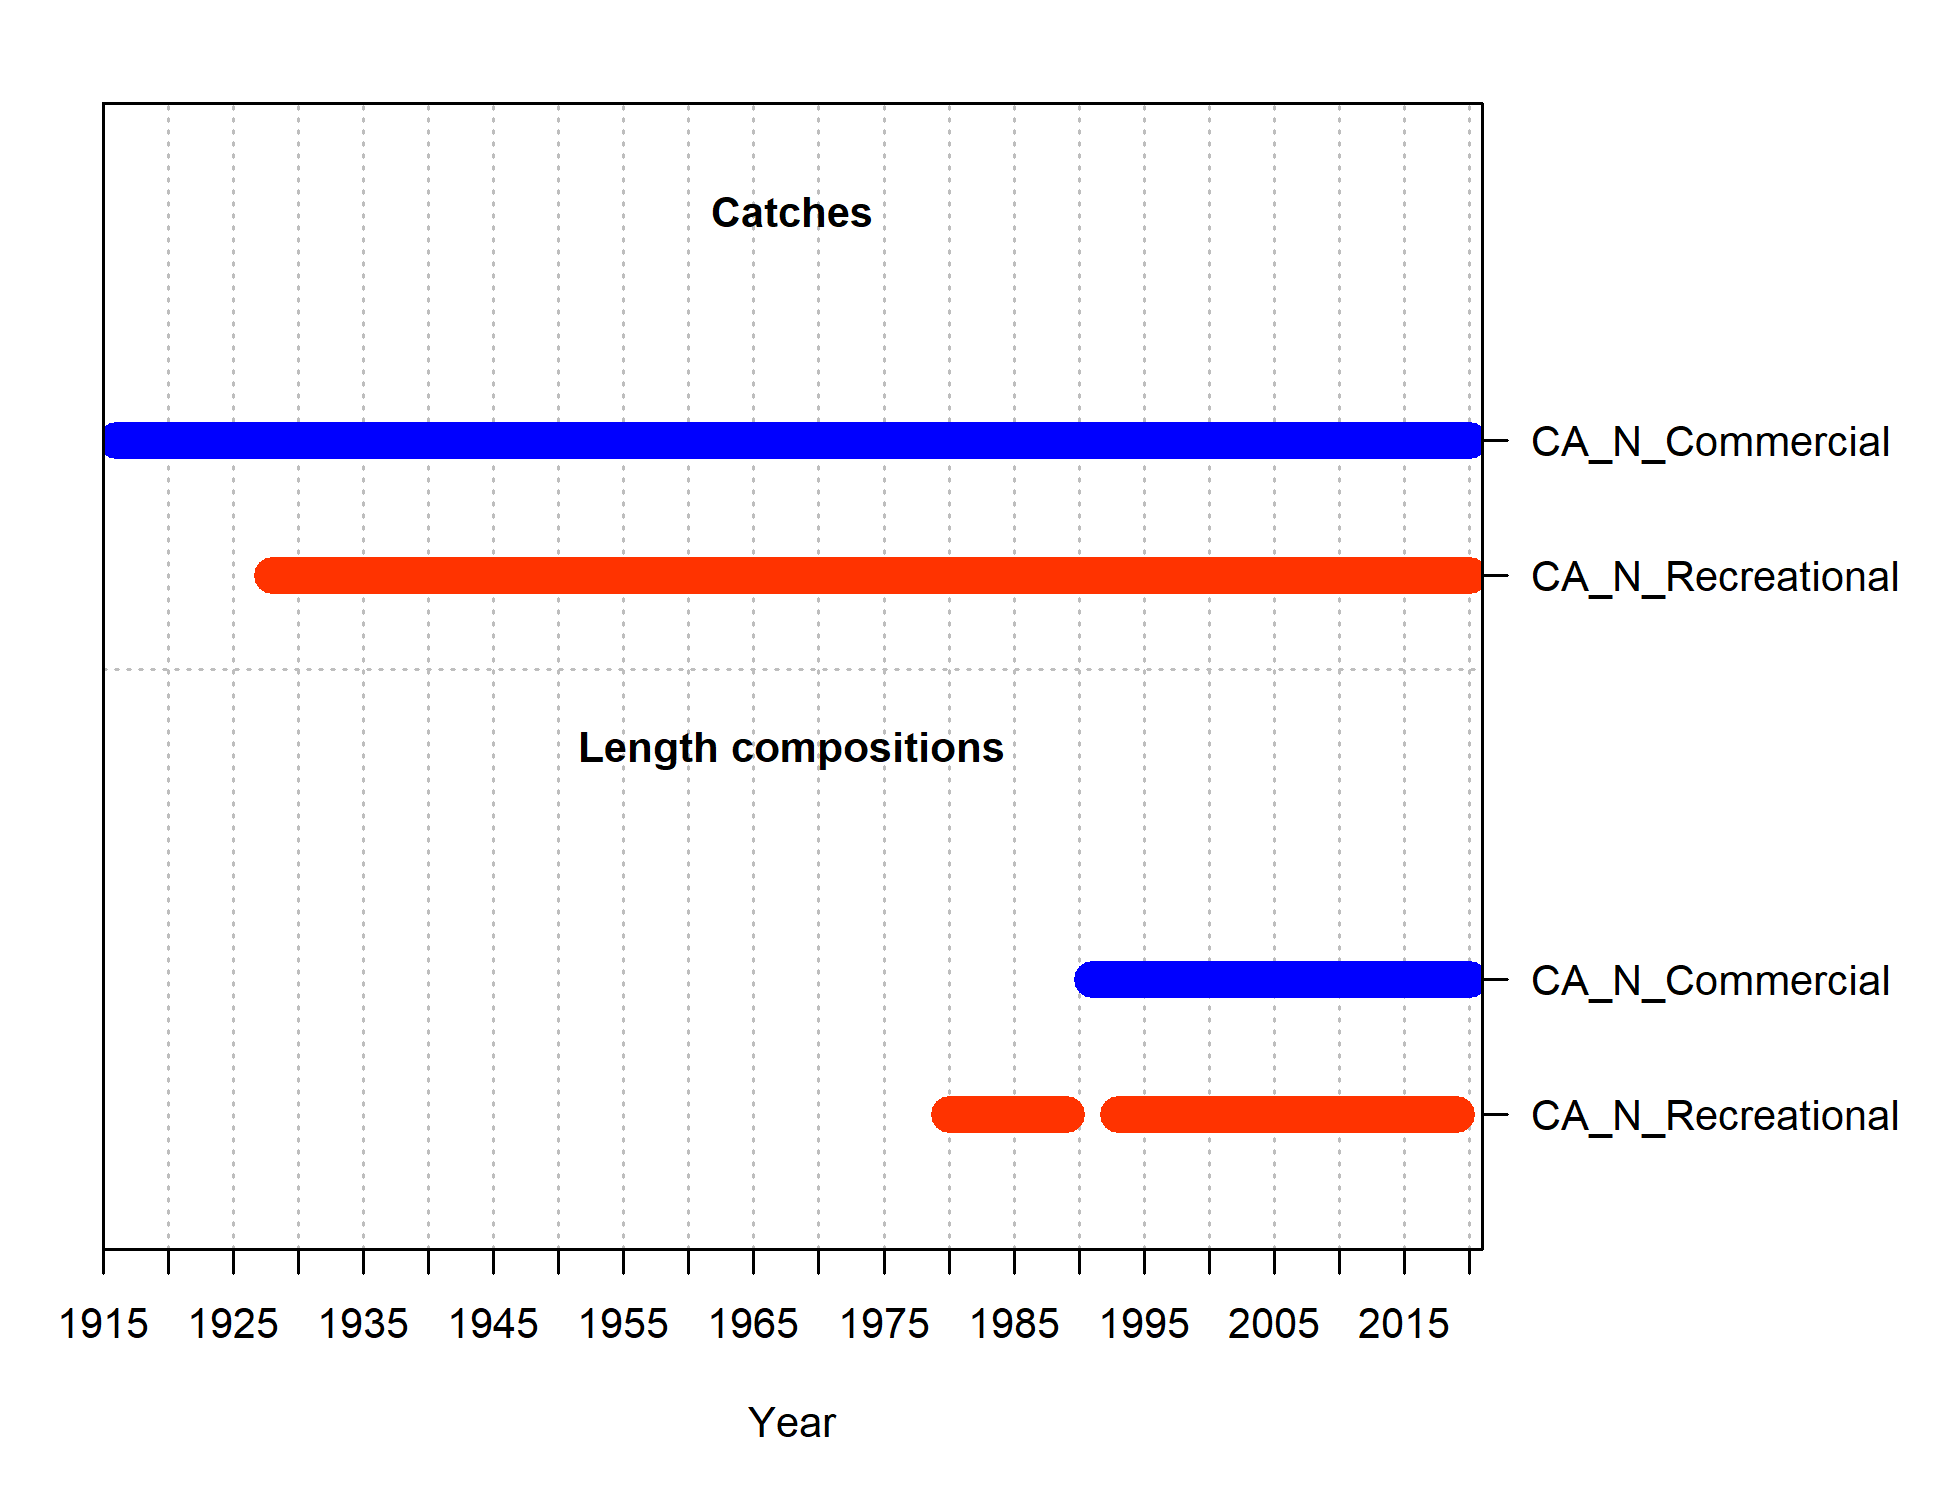
\includegraphics[width=1\textwidth,height=1\textheight]{C:/Assessments/2021/copper_rockfish_2021/write_up/n_ca/figs/data_plot.png}
\caption{Summary of data sources used in the base model.\label{fig:data-plot}}
\end{figure}

\tagmcend\tagstructend

\tagstructbegin{tag=Figure,alttext={Length composition data from the commercial fleet.}}\tagmcbegin{tag=Figure}

\begin{figure}
\centering
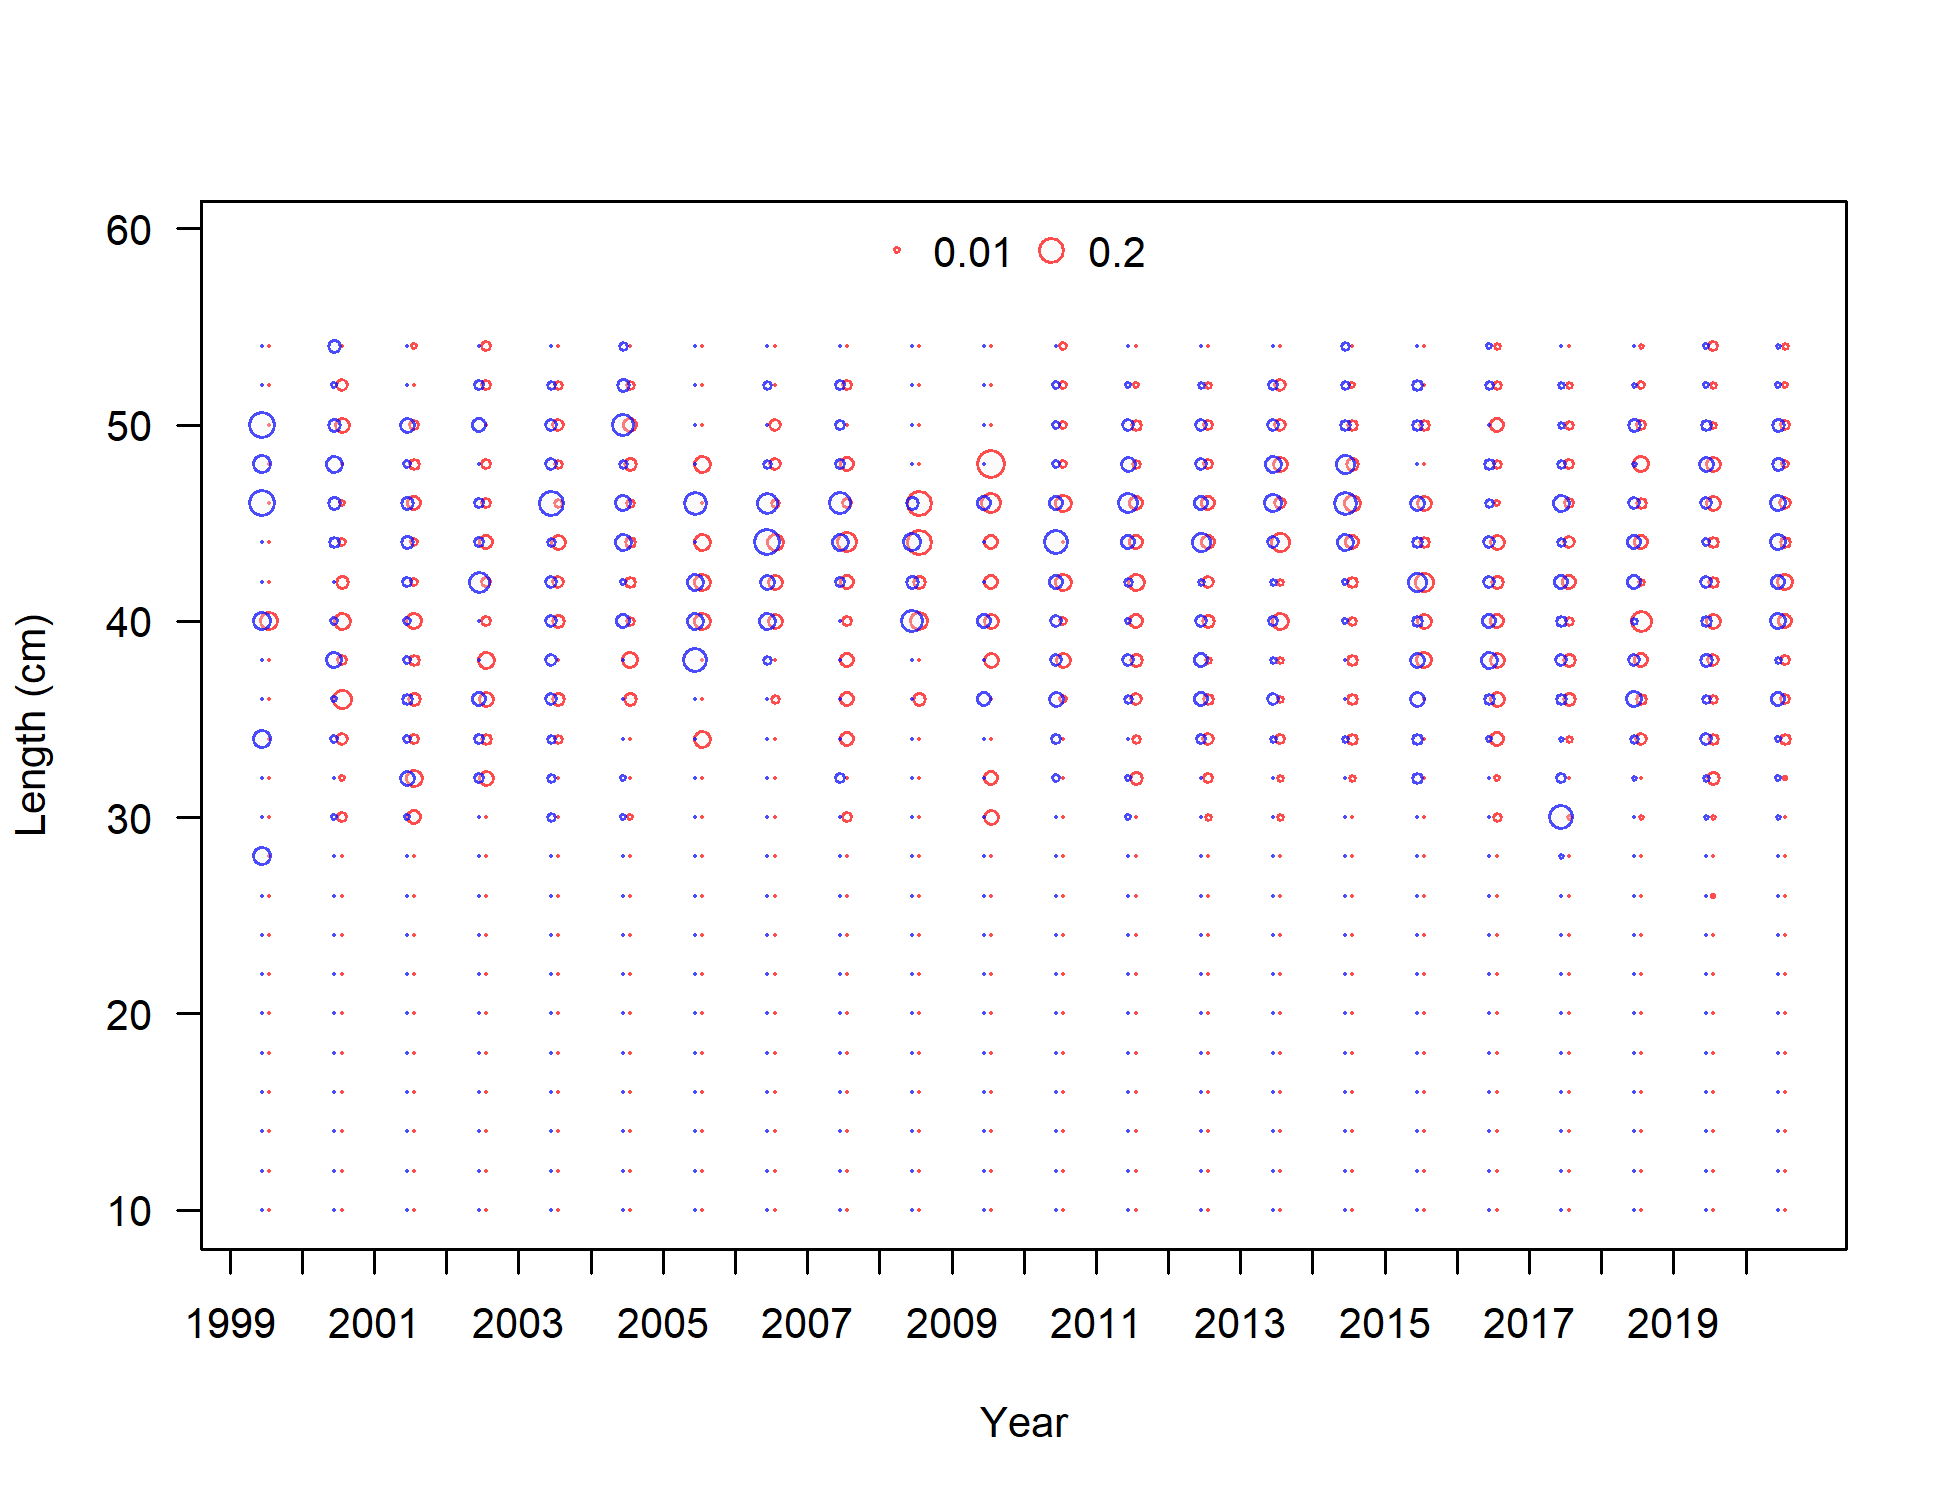
\includegraphics[width=1\textwidth,height=1\textheight]{C:/Assessments/2021/copper_rockfish_2021/models/ca_n_pt_c/10.3_base/plots/comp_lendat_bubflt1mkt0_page2.png}
\caption{Length composition data from the commercial fleet.\label{fig:com-len-data}}
\end{figure}

\tagmcend\tagstructend

\tagstructbegin{tag=Figure,alttext={Mean length for commercial fleet with 95 percent confidence intervals.}}\tagmcbegin{tag=Figure}

\begin{figure}
\centering
\includegraphics[width=1\textwidth,height=1\textheight]{C:/Assessments/2021/copper_rockfish_2021/models/ca_n_pt_c/10.3_base/plots/comp_lendat_data_weighting_TA1.8_CA_N_Commercial.png}
\caption{Mean length for commercial fleet with 95 percent confidence intervals.\label{fig:mean-com-len-data}}
\end{figure}

\tagmcend\tagstructend

\tagstructbegin{tag=Figure,alttext={Length composition data from the recreational fleet.}}\tagmcbegin{tag=Figure}

\begin{figure}
\centering
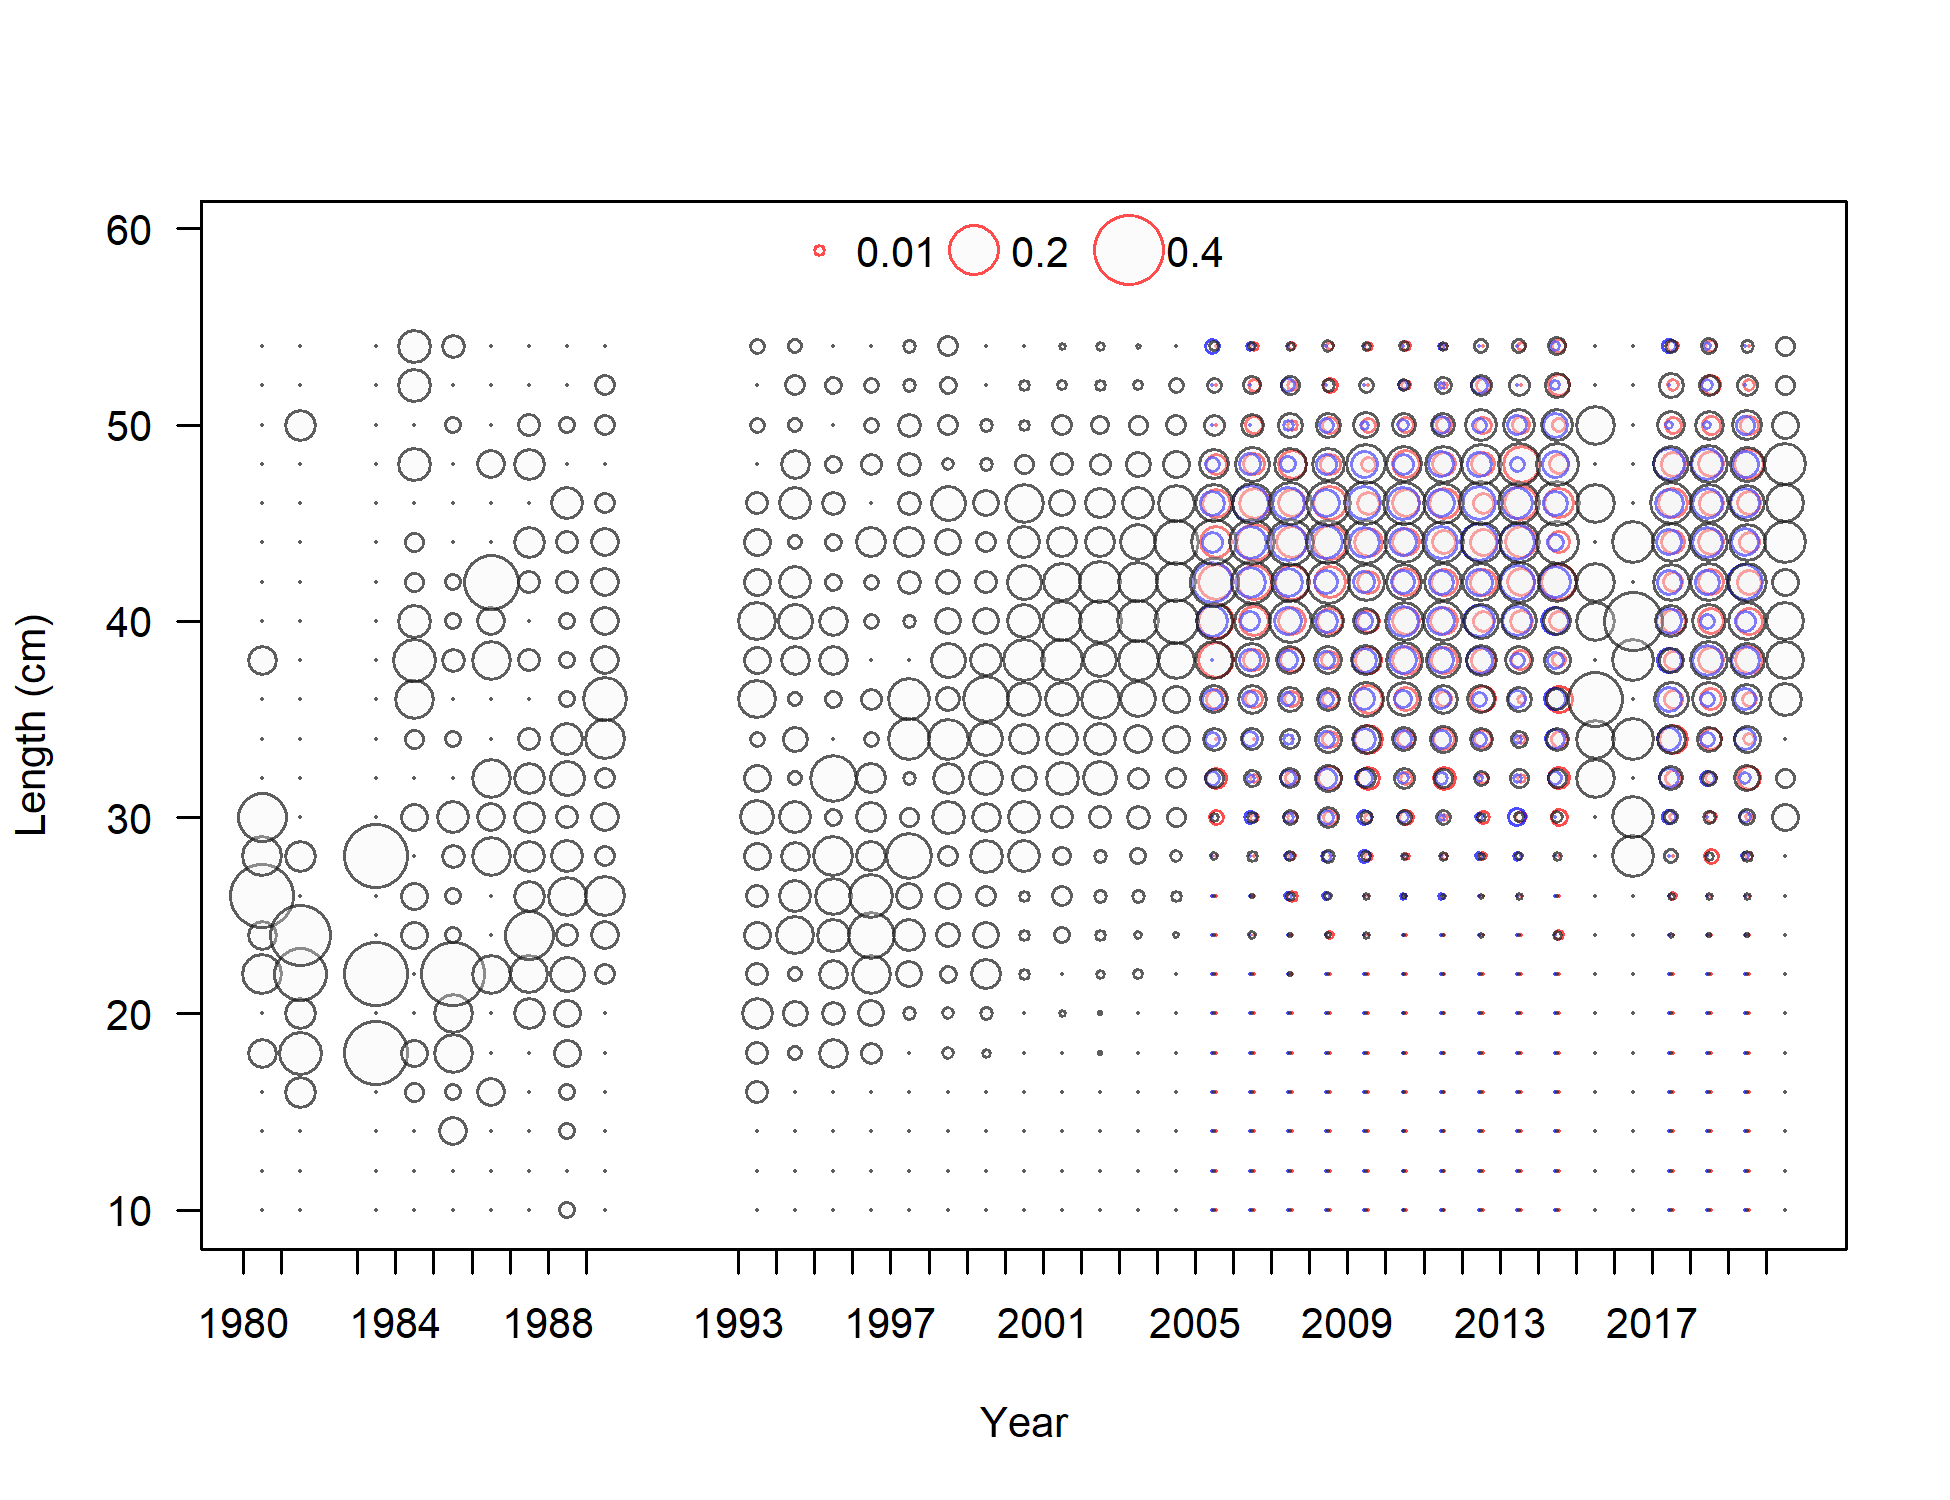
\includegraphics[width=1\textwidth,height=1\textheight]{C:/Assessments/2021/copper_rockfish_2021/models/ca_n_pt_c/10.3_base/plots/comp_lendat_bubflt2mkt0_page3.png}
\caption{Length composition data from the recreational fleet.\label{fig:rec-len-data}}
\end{figure}

\tagmcend\tagstructend

\tagstructbegin{tag=Figure,alttext={Mean length for recreational fleet with 95 percent confidence intervals.}}\tagmcbegin{tag=Figure}

\begin{figure}
\centering
\includegraphics[width=1\textwidth,height=1\textheight]{C:/Assessments/2021/copper_rockfish_2021/models/ca_n_pt_c/10.3_base/plots/comp_lendat_data_weighting_TA1.8_CA_N_Recreational.png}
\caption{Mean length for recreational fleet with 95 percent confidence intervals.\label{fig:mean-rec-len-data}}
\end{figure}

\tagmcend\tagstructend

\tagstructbegin{tag=Figure,alttext={Length frequency distribution in each 10 fm depth bin for copper rockfish sampled by the ROV in reference locations open to fishing north of Point Conception.}}\tagmcbegin{tag=Figure}

\begin{figure}
\centering
\includegraphics[width=1\textwidth,height=1\textheight]{//nwcfile/FRAM/Assessments/CurrentAssessments/DataModerate_2021/copper_rockfish/data/survey/rov/copper_nocal_open_area.png}
\caption{Length frequency distribution in each 10 fm depth bin for copper rockfish sampled by the ROV in reference locations open to fishing north of Point Conception.\label{fig:rov-open}}
\end{figure}

\tagmcend\tagstructend

\clearpage

\tagstructbegin{tag=Figure,alttext={Length frequency distribution in each 10 fm depth bin for copper rockfish sampled by the ROV in marine protected areas where fishing for groundfish is prohibited.}}\tagmcbegin{tag=Figure}

\begin{figure}
\centering
\includegraphics[width=1\textwidth,height=1\textheight]{//nwcfile/FRAM/Assessments/CurrentAssessments/DataModerate_2021/copper_rockfish/data/survey/rov/copper_nocal_mpa_area.png}
\caption{Length frequency distribution in each 10 fm depth bin for copper rockfish sampled by the ROV in marine protected areas where fishing for groundfish is prohibited.\label{fig:rov-mpa}}
\end{figure}

\tagmcend\tagstructend

\clearpage

\tagstructbegin{tag=Figure,alttext={Percent composition of copper rockfish length frequency in 5 cm size classes for each 10 fm depth bin from ROV observations north of Point Conception in reference locations where where fishing for groundfish is allowed.}}\tagmcbegin{tag=Figure}

\begin{figure}
\centering
\includegraphics[width=1\textwidth,height=1\textheight]{//nwcfile/FRAM/Assessments/CurrentAssessments/DataModerate_2021/copper_rockfish/data/survey/rov/copper_nocal_percent_open.png}
\caption{Percent composition of copper rockfish length frequency in 5 cm size classes for each 10 fm depth bin from ROV observations north of Point Conception in reference locations where where fishing for groundfish is allowed.\label{fig:rov-percent-open}}
\end{figure}

\tagmcend\tagstructend

\clearpage

\tagstructbegin{tag=Figure,alttext={Percent composition of copper rockfish length frequency in 5 cm size classes for each 10 fm depth bin from ROV observations north of Point Conception in marine protected areas where where fishing for groundfish is prohibited.}}\tagmcbegin{tag=Figure}

\begin{figure}
\centering
\includegraphics[width=1\textwidth,height=1\textheight]{//nwcfile/FRAM/Assessments/CurrentAssessments/DataModerate_2021/copper_rockfish/data/survey/rov/copper_nocal_percent_mpa.png}
\caption{Percent composition of copper rockfish length frequency in 5 cm size classes for each 10 fm depth bin from ROV observations north of Point Conception in marine protected areas where where fishing for groundfish is prohibited.\label{fig:rov-percent-mpa}}
\end{figure}

\tagmcend\tagstructend

\tagstructbegin{tag=Figure,alttext={Comparison of the length-at-weight data from the NWFSC Hook and Line and the NWFSC WCGBT surveys.}}\tagmcbegin{tag=Figure}

\begin{figure}
\centering
\includegraphics[width=1\textwidth,height=1\textheight]{//nwcfile/FRAM/Assessments/CurrentAssessments/DataModerate_2021/copper_rockfish/data/biology/plots/doc_Length_Weight_Source.png}
\caption{Comparison of the length-at-weight data from the NWFSC Hook and Line and the NWFSC WCGBT surveys.\label{fig:len-weight-survey}}
\end{figure}

\tagmcend\tagstructend

\tagstructbegin{tag=Figure,alttext={Weight-at-length by sex used in the model.}}\tagmcbegin{tag=Figure}

\begin{figure}
\centering
\includegraphics[width=1\textwidth,height=1\textheight]{C:/Assessments/2021/copper_rockfish_2021/models/ca_n_pt_c/10.3_base/plots/bio5_weightatsize.png}
\caption{Weight-at-length by sex used in the model.\label{fig:len-weight}}
\end{figure}

\tagmcend\tagstructend

\tagstructbegin{tag=Figure,alttext={Observed sex specific length-at-age by data source with the estimate length-at-age curve.}}\tagmcbegin{tag=Figure}

\begin{figure}
\centering
\includegraphics[width=1\textwidth,height=1\textheight]{//nwcfile/FRAM/Assessments/CurrentAssessments/DataModerate_2021/copper_rockfish/data/biology/plots/doc_north_Age_by_Sex_Source.png}
\caption{Observed sex specific length-at-age by data source with the estimate length-at-age curve.\label{fig:len-age-data}}
\end{figure}

\tagmcend\tagstructend

\tagstructbegin{tag=Figure,alttext={Length at age in the beginning of the year in the ending year of the model.}}\tagmcbegin{tag=Figure}

\begin{figure}
\centering
\includegraphics[width=1\textwidth,height=1\textheight]{C:/Assessments/2021/copper_rockfish_2021/models/ca_n_pt_c/10.3_base/plots/bio1_sizeatage.png}
\caption{Length at age in the beginning of the year in the ending year of the model.\label{fig:len-age-ss}}
\end{figure}

\tagmcend\tagstructend

\clearpage

\tagstructbegin{tag=Figure,alttext={Maturity as a function of  length.}}\tagmcbegin{tag=Figure}

\begin{figure}
\centering
\includegraphics[width=1\textwidth,height=1\textheight]{C:/Assessments/2021/copper_rockfish_2021/models/ca_n_pt_c/10.3_base/plots/bio6_maturity.png}
\caption{Maturity as a function of length.\label{fig:maturity}}
\end{figure}

\tagmcend\tagstructend

\clearpage

\tagstructbegin{tag=Figure,alttext={Fecundity as a function of length.}}\tagmcbegin{tag=Figure}

\begin{figure}
\centering
\includegraphics[width=1\textwidth,height=1\textheight]{C:/Assessments/2021/copper_rockfish_2021/models/ca_n_pt_c/10.3_base/plots/bio9_fecundity_len.png}
\caption{Fecundity as a function of length.\label{fig:fecundity}}
\end{figure}

\tagmcend\tagstructend

\clearpage

\tagstructbegin{tag=Figure,alttext={Fraction female by length across all available data sources.}}\tagmcbegin{tag=Figure}

\begin{figure}
\centering
\includegraphics[width=1\textwidth,height=1\textheight]{//nwcfile/FRAM/Assessments/CurrentAssessments/DataModerate_2021/copper_rockfish/data/biology/plots/Length_fraction_female.png}
\caption{Fraction female by length across all available data sources.\label{fig:len-sex-ratio}}
\end{figure}

\tagmcend\tagstructend

\tagstructbegin{tag=Figure,alttext={Fraction female by age across all available data sources.}}\tagmcbegin{tag=Figure}

\begin{figure}
\centering
\includegraphics[width=1\textwidth,height=1\textheight]{//nwcfile/FRAM/Assessments/CurrentAssessments/DataModerate_2021/copper_rockfish/data/biology/plots/Age_fraction_female.png}
\caption{Fraction female by age across all available data sources.\label{fig:age-sex-ratio}}
\end{figure}

\tagmcend\tagstructend

\tagstructbegin{tag=Figure,alttext={Selectivity at length by fleet.}}\tagmcbegin{tag=Figure}

\begin{figure}
\centering
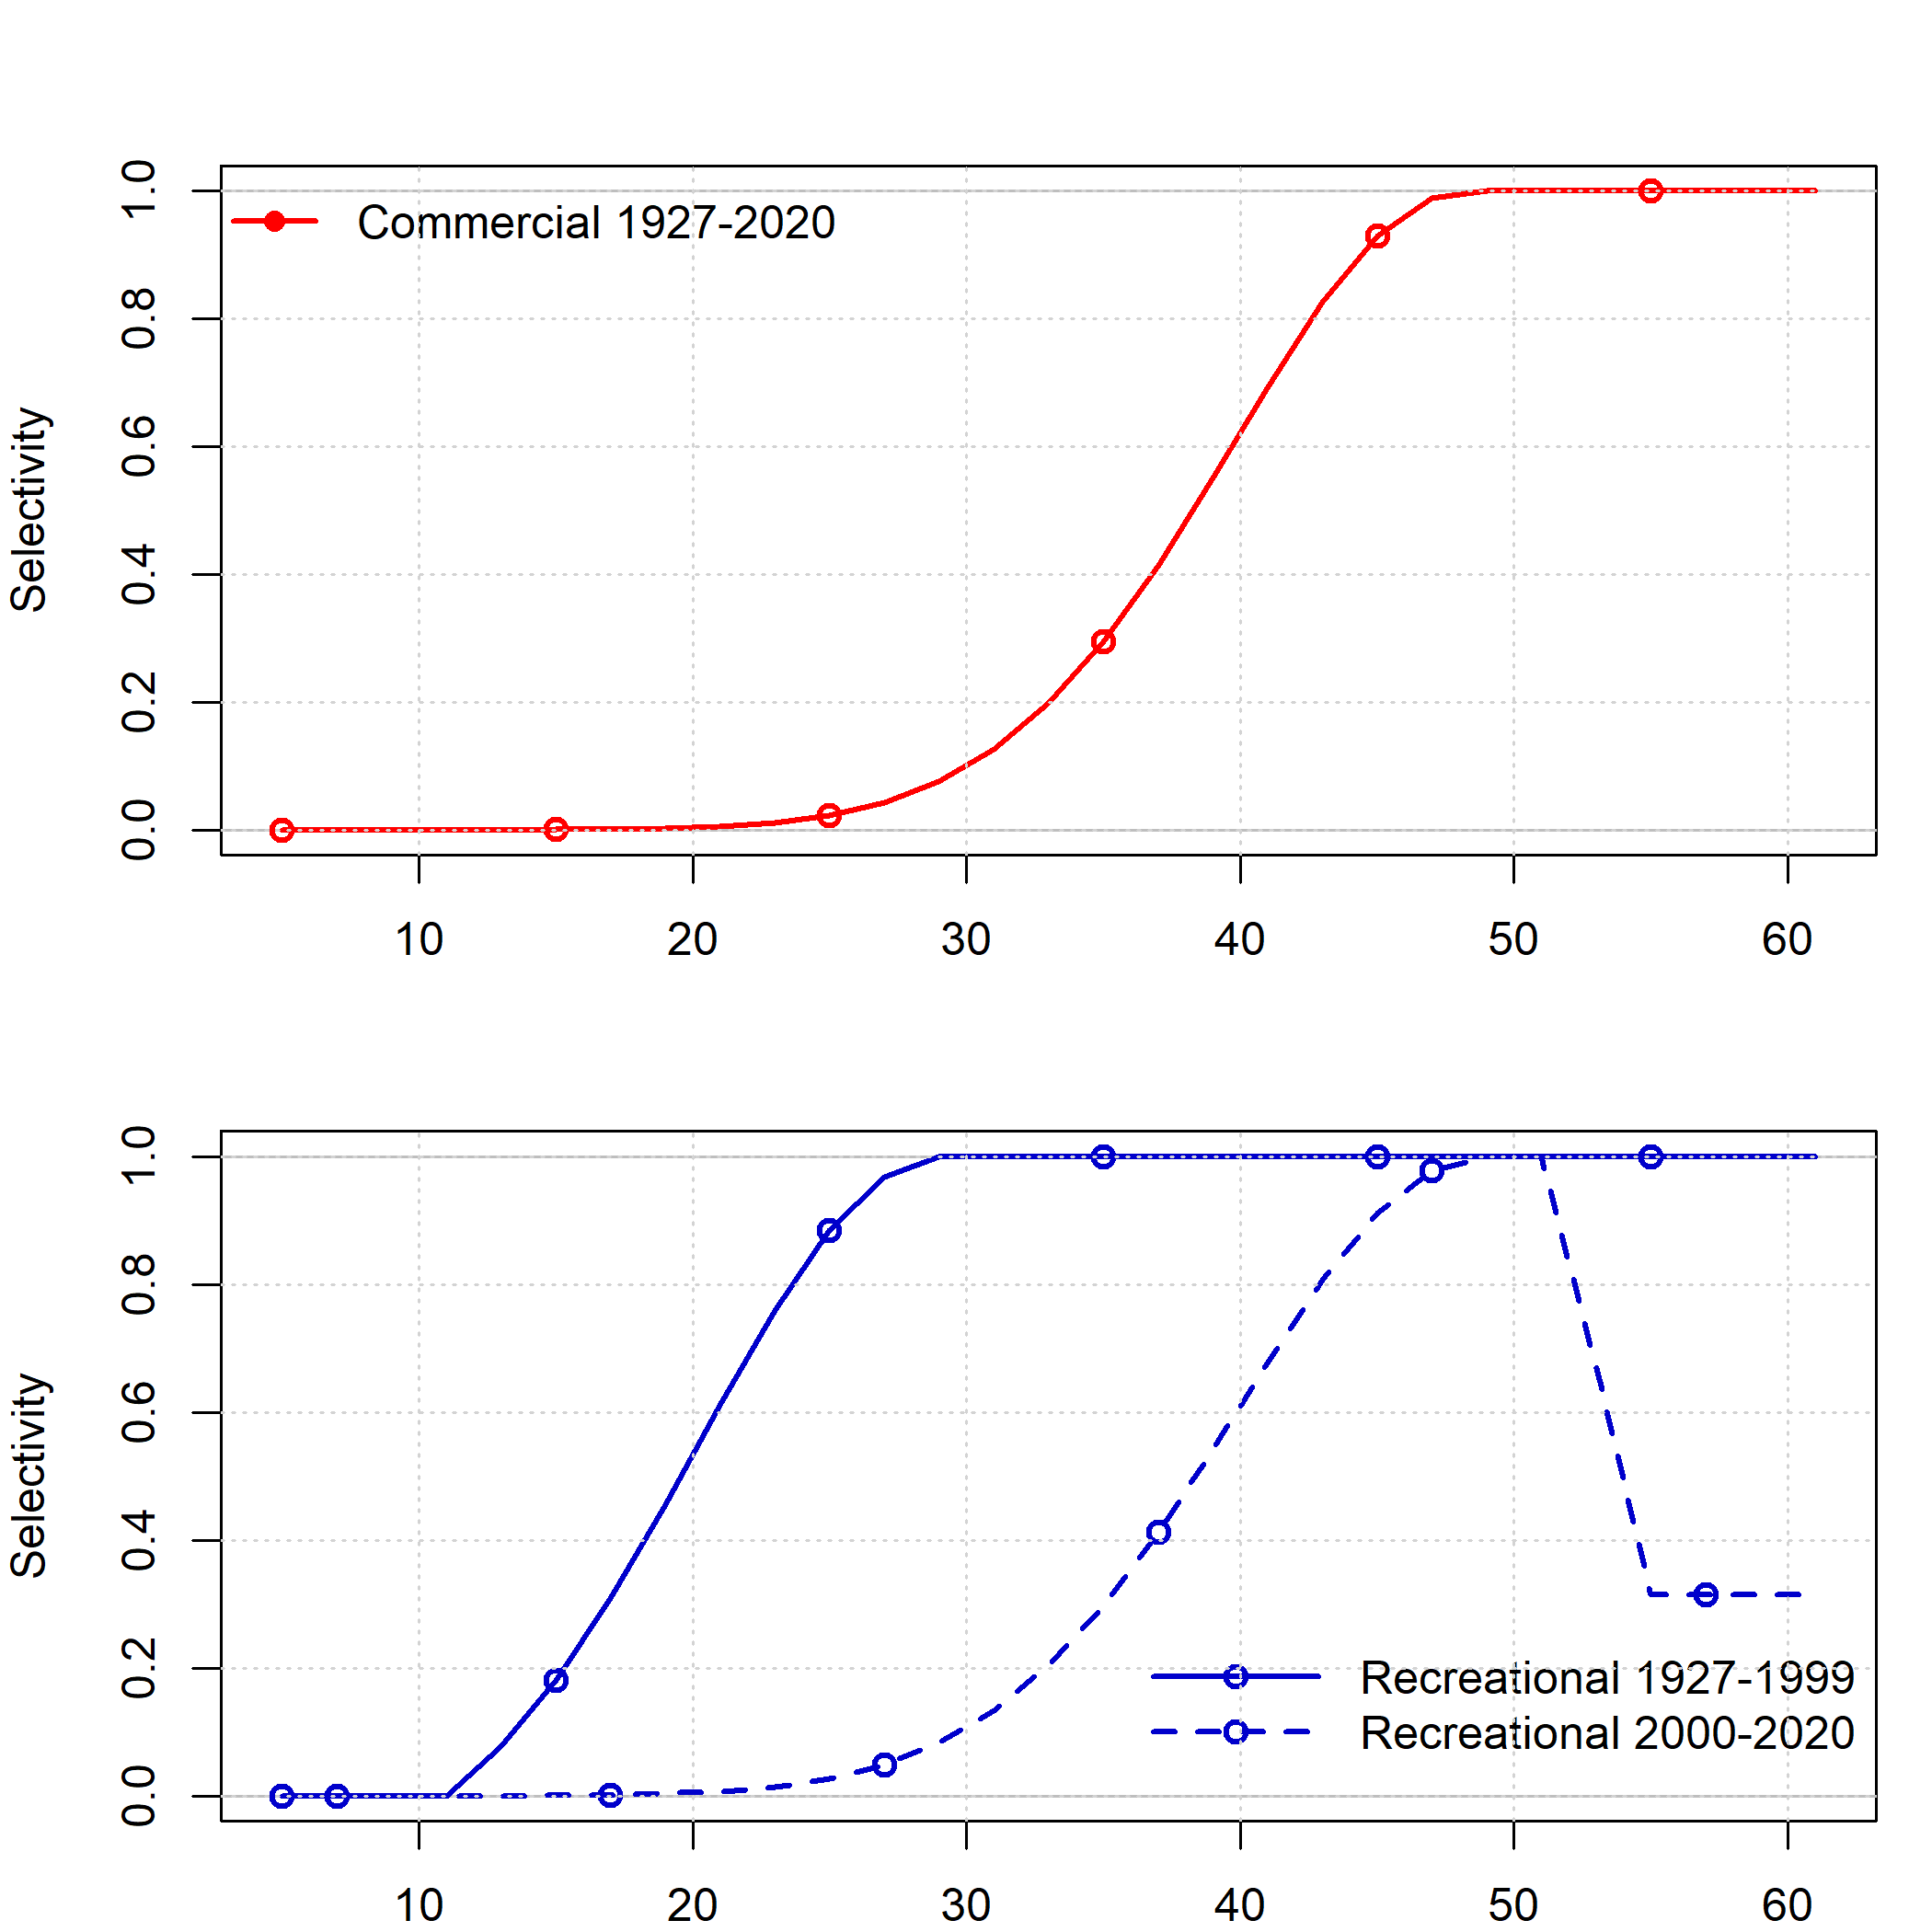
\includegraphics[width=1\textwidth,height=1\textheight]{C:/Assessments/2021/copper_rockfish_2021/write_up/n_ca/figs/selectivity.png}
\caption{Selectivity at length by fleet.\label{fig:selex}}
\end{figure}

\tagmcend\tagstructend

\tagstructbegin{tag=Figure,alttext={Estimated time series of age-0 recruits (1000s).}}\tagmcbegin{tag=Figure}

\begin{figure}
\centering
\includegraphics[width=1\textwidth,height=1\textheight]{C:/Assessments/2021/copper_rockfish_2021/models/ca_n_pt_c/10.3_base/plots/ts11_Age-0_recruits_(1000s)_with_95_asymptotic_intervals.png}
\caption{Estimated time series of age-0 recruits (1000s).\label{fig:recruits}}
\end{figure}

\tagmcend\tagstructend

\tagstructbegin{tag=Figure,alttext={Estimated time series of recruitment deviations.}}\tagmcbegin{tag=Figure}

\begin{figure}
\centering
\includegraphics[width=1\textwidth,height=1\textheight]{C:/Assessments/2021/copper_rockfish_2021/models/ca_n_pt_c/10.3_base/plots/recdevs2_withbars.png}
\caption{Estimated time series of recruitment deviations.\label{fig:rec-devs}}
\end{figure}

\tagmcend\tagstructend

\tagstructbegin{tag=Figure,alttext={Recruitment bias adjustment applied in the base model.}}\tagmcbegin{tag=Figure}

\begin{figure}
\centering
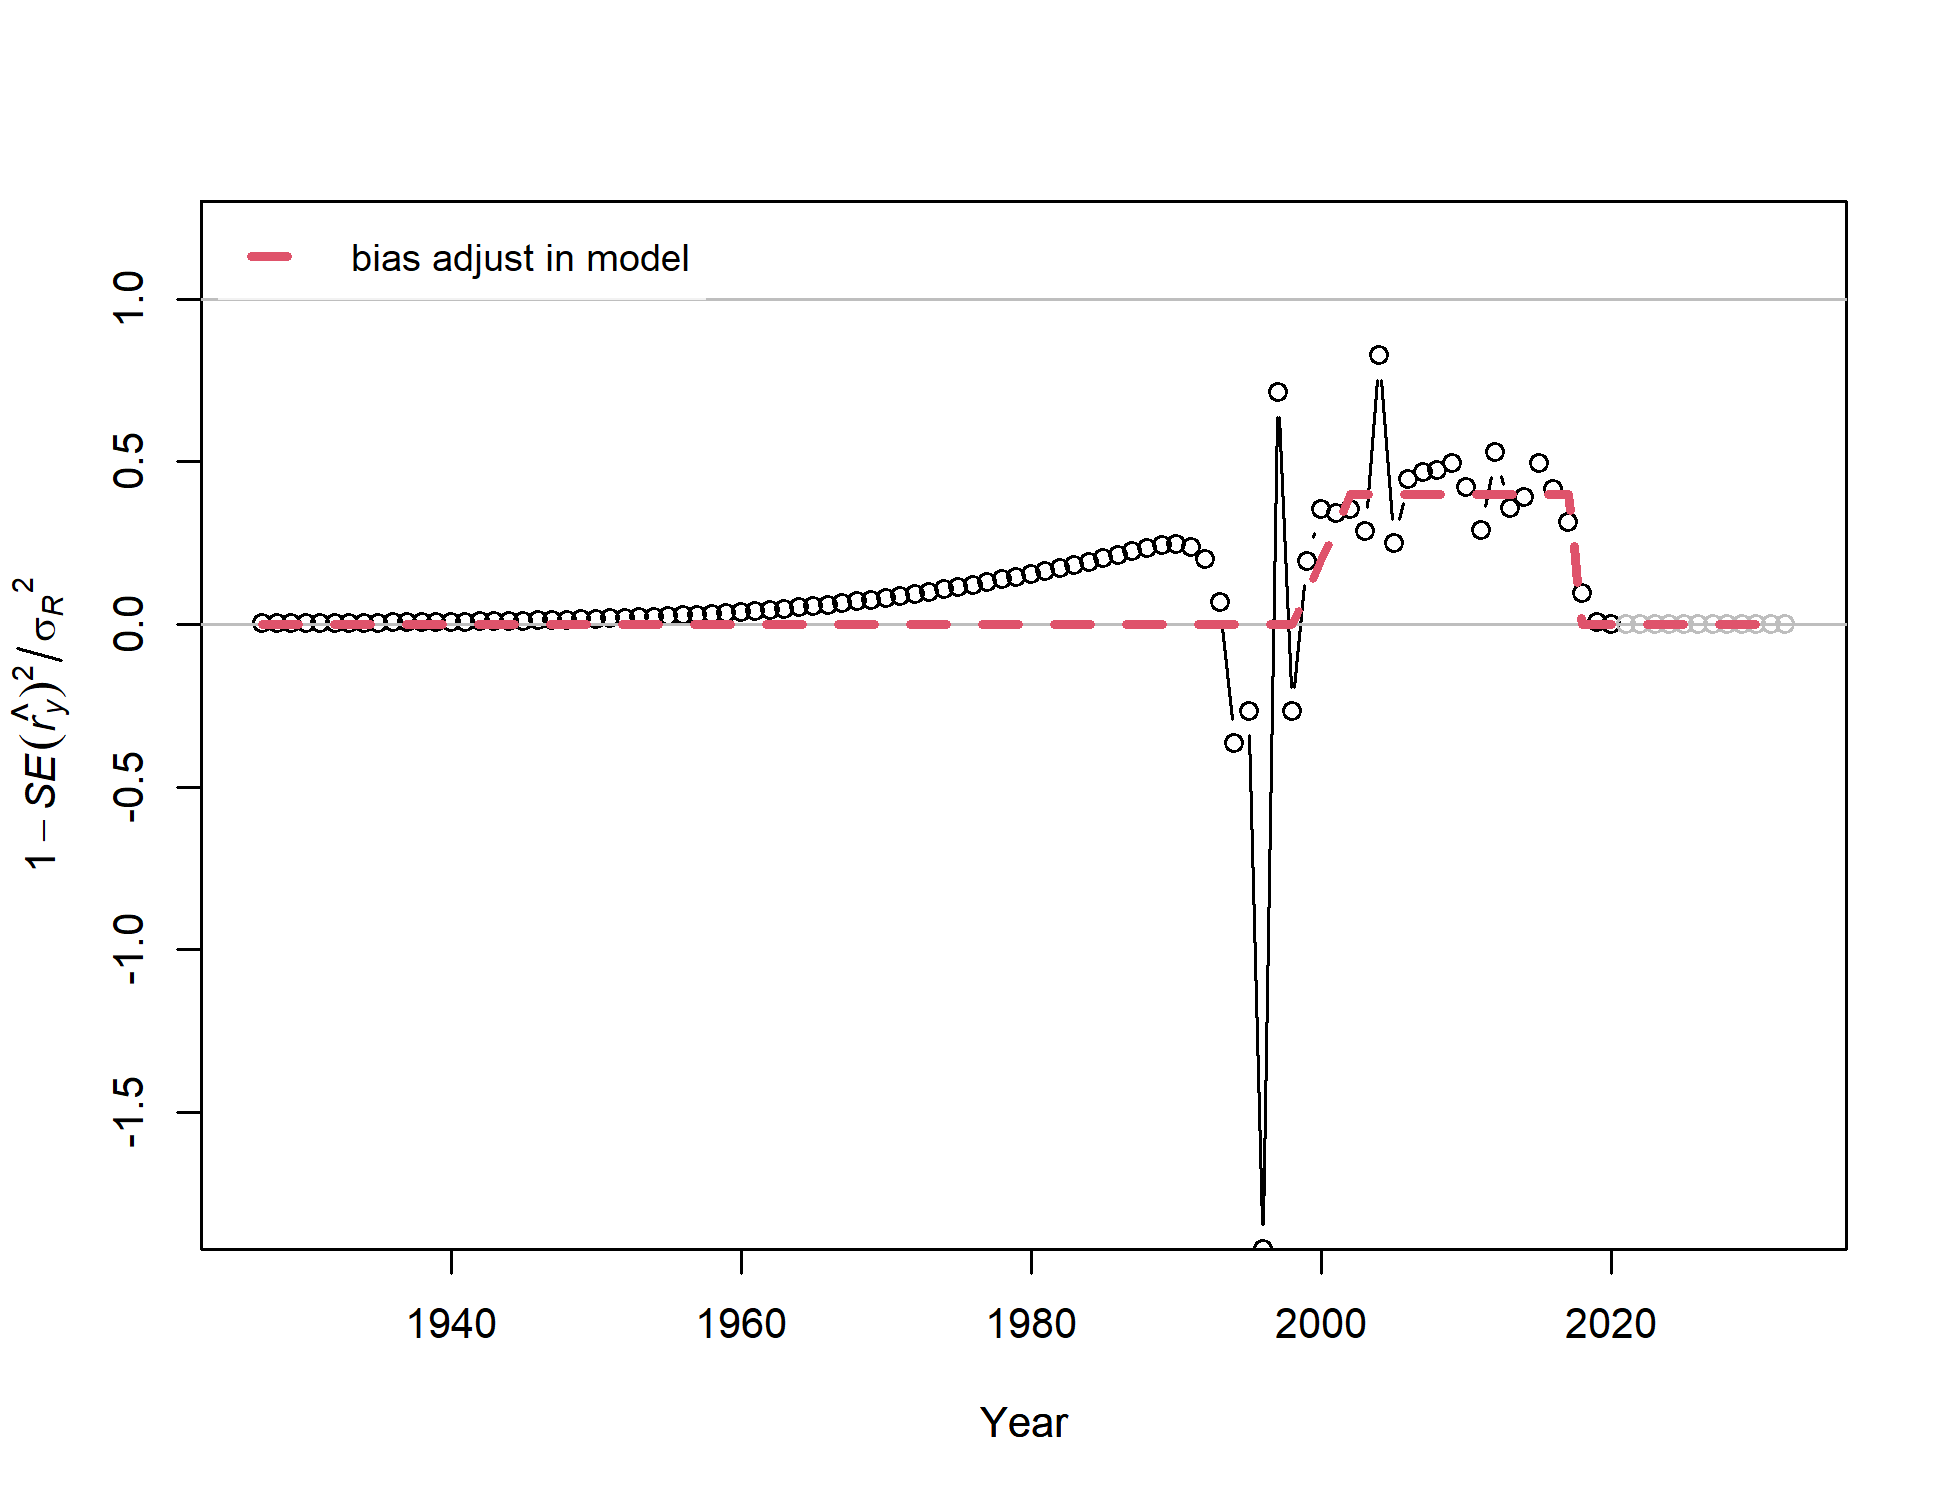
\includegraphics[width=1\textwidth,height=1\textheight]{C:/Assessments/2021/copper_rockfish_2021/write_up/n_ca/figs/recruit_fit_bias_adjust.png}
\caption{Recruitment bias adjustment applied in the base model.\label{fig:bias-adj}}
\end{figure}

\tagmcend\tagstructend

\tagstructbegin{tag=Figure,alttext={Stock-recruit curve. Point colors indicate year, with warmer colors indicating earlier years and cooler colors in showing later years.}}\tagmcbegin{tag=Figure}

\begin{figure}
\centering
\includegraphics[width=1\textwidth,height=1\textheight]{C:/Assessments/2021/copper_rockfish_2021/models/ca_n_pt_c/10.3_base/plots/SR_curve.png}
\caption{Stock-recruit curve. Point colors indicate year, with warmer colors indicating earlier years and cooler colors in showing later years.\label{fig:bh-curve}}
\end{figure}

\tagmcend\tagstructend

\tagstructbegin{tag=Figure,alttext={Pearson residuals for commercial fleet. Closed bubble are positive residuals (observed > expected) and open bubbles are negative residuals (observed < expected).}}\tagmcbegin{tag=Figure}

\begin{figure}
\centering
\includegraphics[width=1\textwidth,height=1\textheight]{C:/Assessments/2021/copper_rockfish_2021/models/ca_n_pt_c/10.3_base/plots/comp_lenfit_residsflt1mkt0_page2.png}
\caption{Pearson residuals for commercial fleet. Closed bubble are positive residuals (observed \textgreater{} expected) and open bubbles are negative residuals (observed \textless{} expected).\label{fig:com-pearson}}
\end{figure}

\tagmcend\tagstructend

\tagstructbegin{tag=Figure,alttext={Mean length for commercial lengths with 95 percent confidence intervals based on current samples sizes.}}\tagmcbegin{tag=Figure}

\begin{figure}
\centering
\includegraphics[width=1\textwidth,height=1\textheight]{C:/Assessments/2021/copper_rockfish_2021/models/ca_n_pt_c/10.3_base/plots/comp_lenfit_data_weighting_TA1.8_CA_N_Commercial.png}
\caption{Mean length for commercial lengths with 95 percent confidence intervals based on current samples sizes.\label{fig:com-mean-len-fit}}
\end{figure}

\tagmcend\tagstructend

\tagstructbegin{tag=Figure,alttext={Pearson residuals for recreational fleet. Closed bubble are positive residuals (observed > expected) and open bubbles are negative residuals (observed < expected).}}\tagmcbegin{tag=Figure}

\begin{figure}
\centering
\includegraphics[width=1\textwidth,height=1\textheight]{C:/Assessments/2021/copper_rockfish_2021/models/ca_n_pt_c/10.3_base/plots/comp_lenfit_residsflt2mkt0_page3.png}
\caption{Pearson residuals for recreational fleet. Closed bubble are positive residuals (observed \textgreater{} expected) and open bubbles are negative residuals (observed \textless{} expected).\label{fig:rec-pearson}}
\end{figure}

\tagmcend\tagstructend

\tagstructbegin{tag=Figure,alttext={Mean length for recreational lengths with 95 percent confidence intervals based on current samples sizes.}}\tagmcbegin{tag=Figure}

\begin{figure}
\centering
\includegraphics[width=1\textwidth,height=1\textheight]{C:/Assessments/2021/copper_rockfish_2021/models/ca_n_pt_c/10.3_base/plots/comp_lenfit_data_weighting_TA1.8_CA_N_Recreational.png}
\caption{Mean length for recreational lengths with 95 percent confidence intervals based on current samples sizes.\label{fig:rec-mean-len-fit}}
\end{figure}

\tagmcend\tagstructend

\tagstructbegin{tag=Figure,alttext={Aggregated length comps across all years.}}\tagmcbegin{tag=Figure}

\begin{figure}
\centering
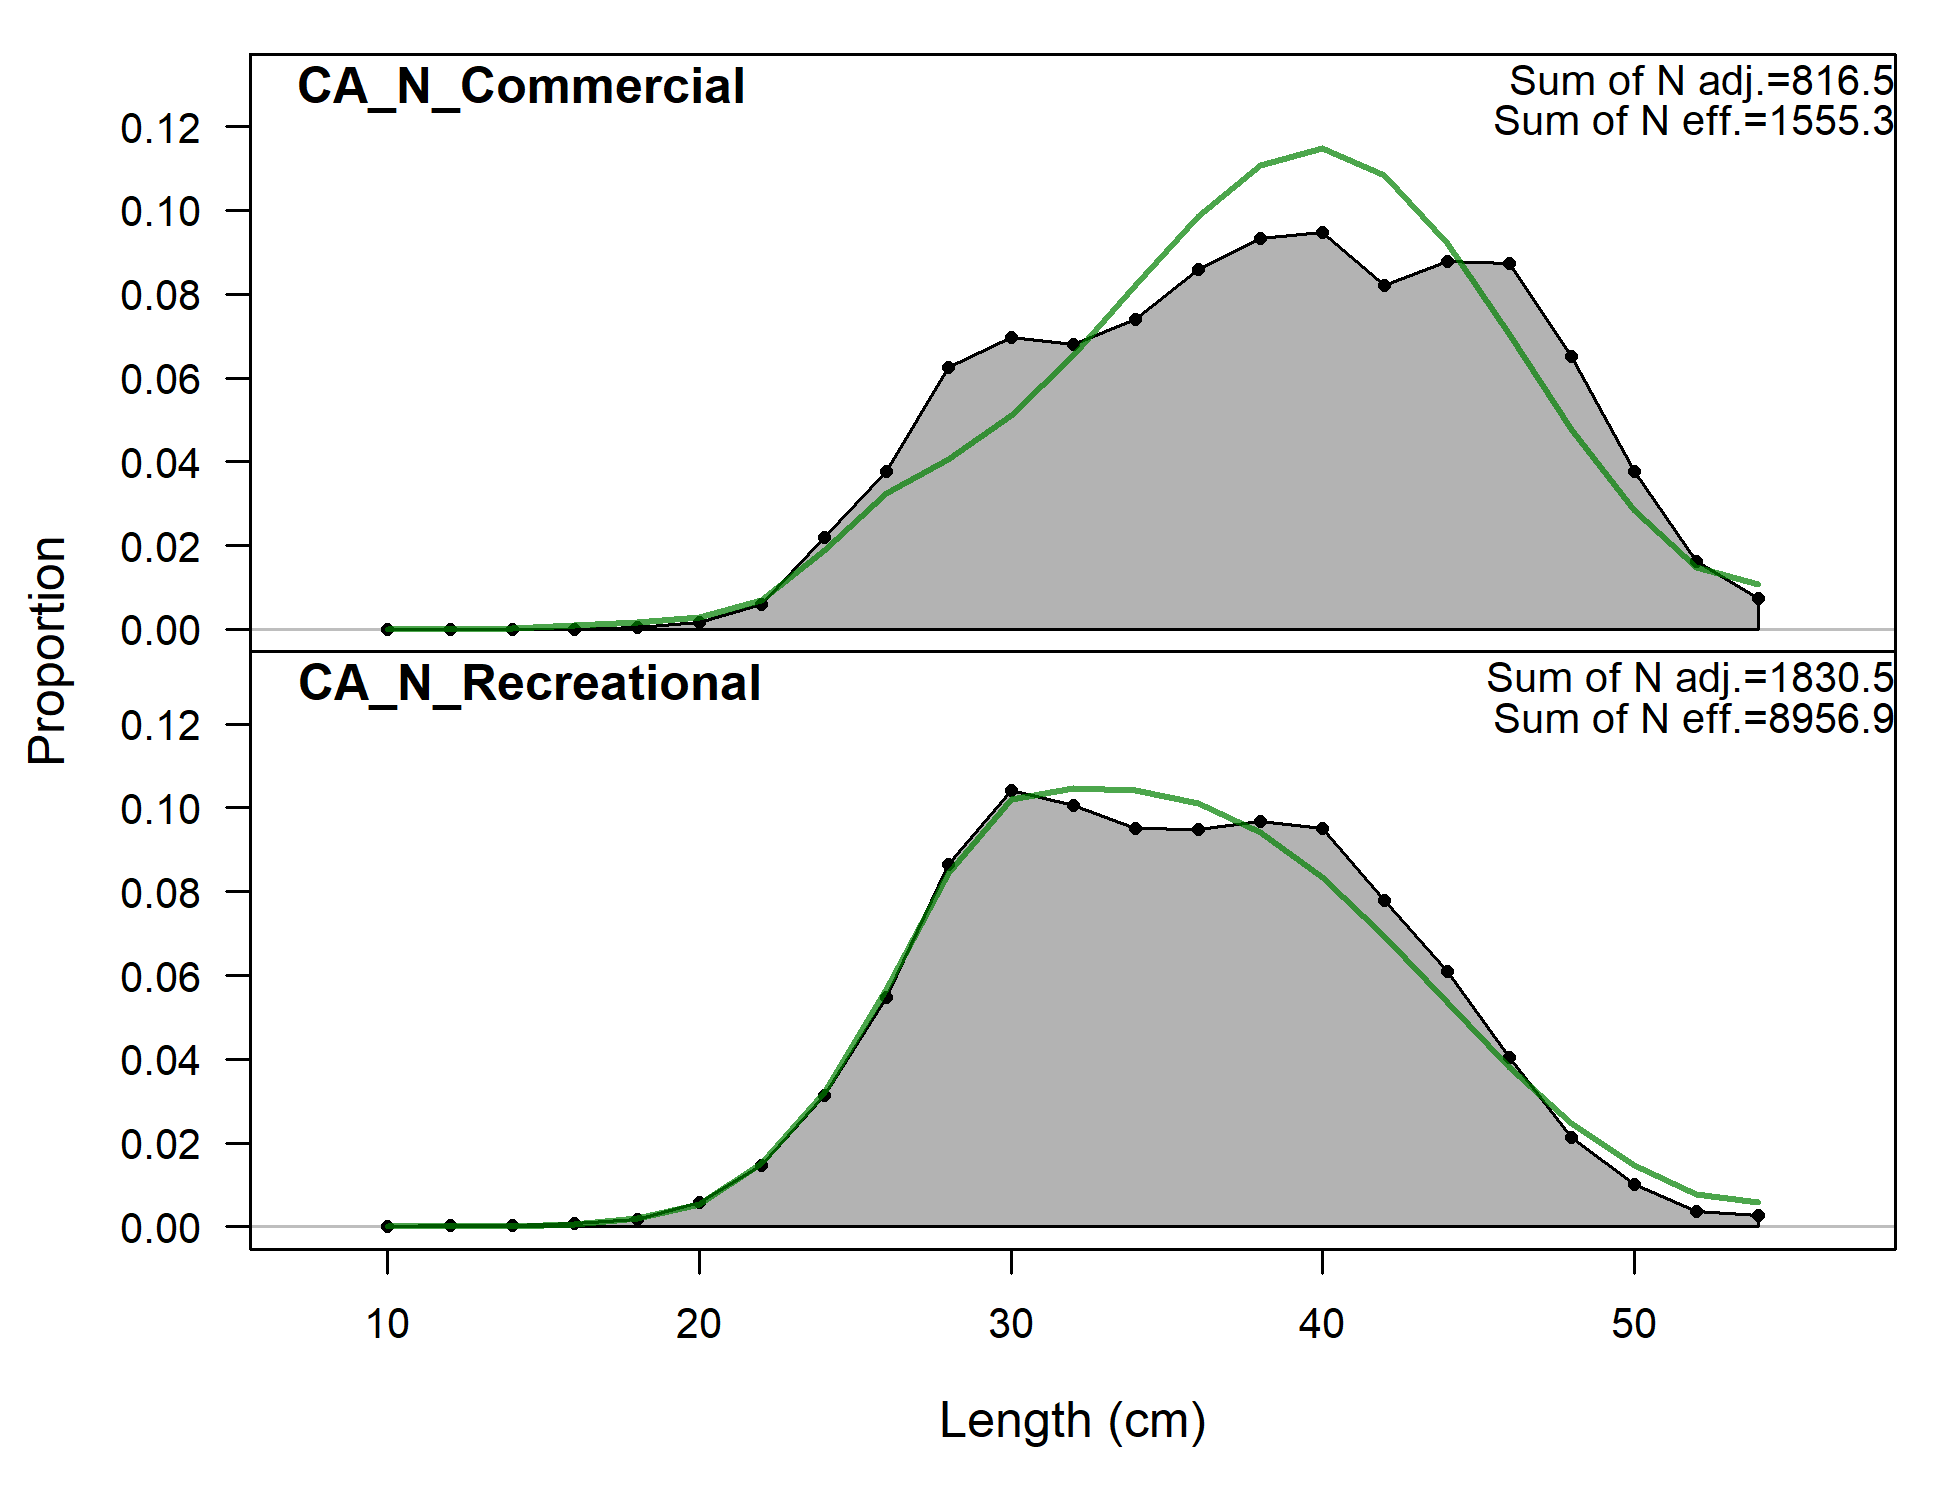
\includegraphics[width=1\textwidth,height=1\textheight]{C:/Assessments/2021/copper_rockfish_2021/models/ca_n_pt_c/10.3_base/plots/comp_lenfit__aggregated_across_time.png}
\caption{Aggregated length comps across all years.\label{fig:agg-len-fit}}
\end{figure}

\tagmcend\tagstructend

\tagstructbegin{tag=Figure,alttext={Estimated time series of spawning output.}}\tagmcbegin{tag=Figure}

\begin{figure}
\centering
\includegraphics[width=1\textwidth,height=1\textheight]{C:/Assessments/2021/copper_rockfish_2021/models/ca_n_pt_c/10.3_base/plots/ts7_Spawning_output_with_95_asymptotic_intervals_intervals.png}
\caption{Estimated time series of spawning output.\label{fig:ssb}}
\end{figure}

\tagmcend\tagstructend

\tagstructbegin{tag=Figure,alttext={Estimated time series of total biomass.}}\tagmcbegin{tag=Figure}

\begin{figure}
\centering
\includegraphics[width=1\textwidth,height=1\textheight]{C:/Assessments/2021/copper_rockfish_2021/models/ca_n_pt_c/10.3_base/plots/ts1_Total_biomass_(mt).png}
\caption{Estimated time series of total biomass.\label{fig:tot-bio}}
\end{figure}

\tagmcend\tagstructend

\tagstructbegin{tag=Figure,alttext={Estimated time series of fraction of unfished spawning output.}}\tagmcbegin{tag=Figure}

\begin{figure}
\centering
\includegraphics[width=1\textwidth,height=1\textheight]{C:/Assessments/2021/copper_rockfish_2021/models/ca_n_pt_c/10.3_base/plots/ts9_Fraction_of_unfished_with_95_asymptotic_intervals_intervals.png}
\caption{Estimated time series of fraction of unfished spawning output.\label{fig:depl}}
\end{figure}

\tagmcend\tagstructend

\tagstructbegin{tag=Figure,alttext={Change in estimated spawning output by sensitivity.}}\tagmcbegin{tag=Figure}

\begin{figure}
\centering
\includegraphics[width=1\textwidth,height=1\textheight]{C:/Assessments/2021/copper_rockfish_2021/models/ca_n_pt_c/_sensitivities/_plots/10.3_base_1_compare2_spawnbio_uncertainty.png}
\caption{Change in estimated spawning output by sensitivity.\label{fig:sens-ssb-1}}
\end{figure}

\tagmcend\tagstructend

\tagstructbegin{tag=Figure,alttext={Change in estimated fraction unfished by sensitivity.}}\tagmcbegin{tag=Figure}

\begin{figure}
\centering
\includegraphics[width=1\textwidth,height=1\textheight]{C:/Assessments/2021/copper_rockfish_2021/models/ca_n_pt_c/_sensitivities/_plots/10.3_base_1_compare4_Bratio_uncertainty.png}
\caption{Change in estimated fraction unfished by sensitivity.\label{fig:sens-depl-1}}
\end{figure}

\tagmcend\tagstructend

\tagstructbegin{tag=Figure,alttext={Change in estimated spawning output by sensitivity.}}\tagmcbegin{tag=Figure}

\begin{figure}
\centering
\includegraphics[width=1\textwidth,height=1\textheight]{C:/Assessments/2021/copper_rockfish_2021/models/ca_n_pt_c/_sensitivities/_plots/10.3_base_2_compare2_spawnbio_uncertainty.png}
\caption{Change in estimated spawning output by sensitivity.\label{fig:sens-ssb-2}}
\end{figure}

\tagmcend\tagstructend

\tagstructbegin{tag=Figure,alttext={Change in estimated fraction unfished by sensitivity.}}\tagmcbegin{tag=Figure}

\begin{figure}
\centering
\includegraphics[width=1\textwidth,height=1\textheight]{C:/Assessments/2021/copper_rockfish_2021/models/ca_n_pt_c/_sensitivities/_plots/10.3_base_2_compare4_Bratio_uncertainty.png}
\caption{Change in estimated fraction unfished by sensitivity.\label{fig:sens-depl-2}}
\end{figure}

\tagmcend\tagstructend

\tagstructbegin{tag=Figure,alttext={Change in the negative log-likelihood across a range of log(R0) values.}}\tagmcbegin{tag=Figure}

\begin{figure}
\centering
\includegraphics[width=1\textwidth,height=1\textheight]{C:/Assessments/2021/copper_rockfish_2021/models/ca_n_pt_c/10.3_base_profile_SR_LN(R0)/piner_panel_SR_LN(R0).png}
\caption{Change in the negative log-likelihood across a range of log(R0) values.\label{fig:r0-profile}}
\end{figure}

\tagmcend\tagstructend

\tagstructbegin{tag=Figure,alttext={Change in the estimate of spawning output across a range of log(R0) values.}}\tagmcbegin{tag=Figure}

\begin{figure}
\centering
\includegraphics[width=1\textwidth,height=1\textheight]{C:/Assessments/2021/copper_rockfish_2021/models/ca_n_pt_c/10.3_base_profile_SR_LN(R0)/SR_LN(R0)_trajectories_compare1_spawnbio.png}
\caption{Change in the estimate of spawning output across a range of log(R0) values.\label{fig:r0-ssb}}
\end{figure}

\tagmcend\tagstructend

\tagstructbegin{tag=Figure,alttext={Change in the estimate of fraction unfished across a range of log(R0) values.}}\tagmcbegin{tag=Figure}

\begin{figure}
\centering
\includegraphics[width=1\textwidth,height=1\textheight]{C:/Assessments/2021/copper_rockfish_2021/models/ca_n_pt_c/10.3_base_profile_SR_LN(R0)/SR_LN(R0)_trajectories_compare3_Bratio.png}
\caption{Change in the estimate of fraction unfished across a range of log(R0) values.\label{fig:r0-depl}}
\end{figure}

\tagmcend\tagstructend

\tagstructbegin{tag=Figure,alttext={Change in the negative log-likelihood across a range of steepness values.}}\tagmcbegin{tag=Figure}

\begin{figure}
\centering
\includegraphics[width=1\textwidth,height=1\textheight]{C:/Assessments/2021/copper_rockfish_2021/models/ca_n_pt_c/10.3_base_profile_SR_BH_steep/piner_panel_SR_BH_steep.png}
\caption{Change in the negative log-likelihood across a range of steepness values.\label{fig:h-profile}}
\end{figure}

\tagmcend\tagstructend

\tagstructbegin{tag=Figure,alttext={Change in the estimate of spawning output across a range of steepness values.}}\tagmcbegin{tag=Figure}

\begin{figure}
\centering
\includegraphics[width=1\textwidth,height=1\textheight]{C:/Assessments/2021/copper_rockfish_2021/models/ca_n_pt_c/10.3_base_profile_SR_BH_steep/SR_BH_steep_trajectories_compare1_spawnbio.png}
\caption{Change in the estimate of spawning output across a range of steepness values.\label{fig:h-ssb}}
\end{figure}

\tagmcend\tagstructend

\tagstructbegin{tag=Figure,alttext={Change in the estimate of fraction unfished across a range of steepness values.}}\tagmcbegin{tag=Figure}

\begin{figure}
\centering
\includegraphics[width=1\textwidth,height=1\textheight]{C:/Assessments/2021/copper_rockfish_2021/models/ca_n_pt_c/10.3_base_profile_SR_BH_steep/SR_BH_steep_trajectories_compare3_Bratio.png}
\caption{Change in the estimate of fraction unfished across a range of steepness values.\label{fig:h-depl}}
\end{figure}

\tagmcend\tagstructend

\tagstructbegin{tag=Figure,alttext={Change in the negative log-likelihood across a range of female natural mortality values.}}\tagmcbegin{tag=Figure}

\begin{figure}
\centering
\includegraphics[width=1\textwidth,height=1\textheight]{C:/Assessments/2021/copper_rockfish_2021/models/ca_n_pt_c/10.3_base_profile_NatM_p_1_Fem_GP_1/piner_panel_NatM_p_1_Fem_GP_1.png}
\caption{Change in the negative log-likelihood across a range of female natural mortality values.\label{fig:m-profile}}
\end{figure}

\tagmcend\tagstructend

\tagstructbegin{tag=Figure,alttext={Change in the estimate of spawning output across a range of female natural mortality values.}}\tagmcbegin{tag=Figure}

\begin{figure}
\centering
\includegraphics[width=1\textwidth,height=1\textheight]{C:/Assessments/2021/copper_rockfish_2021/models/ca_n_pt_c/10.3_base_profile_NatM_p_1_Fem_GP_1/NatM_p_1_Fem_GP_1_trajectories_compare1_spawnbio.png}
\caption{Change in the estimate of spawning output across a range of female natural mortality values.\label{fig:m-ssb}}
\end{figure}

\tagmcend\tagstructend

\tagstructbegin{tag=Figure,alttext={Change in the estimate of fraction unfished across a range of female natural values.}}\tagmcbegin{tag=Figure}

\begin{figure}
\centering
\includegraphics[width=1\textwidth,height=1\textheight]{C:/Assessments/2021/copper_rockfish_2021/models/ca_n_pt_c/10.3_base_profile_NatM_p_1_Fem_GP_1/NatM_p_1_Fem_GP_1_trajectories_compare3_Bratio.png}
\caption{Change in the estimate of fraction unfished across a range of female natural values.\label{fig:m-depl}}
\end{figure}

\tagmcend\tagstructend

\tagstructbegin{tag=Figure,alttext={Change in the negative log-likelihood across a range of female maximum length values.}}\tagmcbegin{tag=Figure}

\begin{figure}
\centering
\includegraphics[width=1\textwidth,height=1\textheight]{C:/Assessments/2021/copper_rockfish_2021/models/ca_n_pt_c/10.3_base_profile_L_at_Amax_Fem_GP_1/piner_panel_L_at_Amax_Fem_GP_1.png}
\caption{Change in the negative log-likelihood across a range of female maximum length values.\label{fig:linf-profile}}
\end{figure}

\tagmcend\tagstructend

\tagstructbegin{tag=Figure,alttext={Change in the estimate of spawning output across a range of female maximum length values.}}\tagmcbegin{tag=Figure}

\begin{figure}
\centering
\includegraphics[width=1\textwidth,height=1\textheight]{C:/Assessments/2021/copper_rockfish_2021/models/ca_n_pt_c/10.3_base_profile_L_at_Amax_Fem_GP_1/L_at_Amax_Fem_GP_1_trajectories_compare1_spawnbio.png}
\caption{Change in the estimate of spawning output across a range of female maximum length values.\label{fig:linf-ssb}}
\end{figure}

\tagmcend\tagstructend

\tagstructbegin{tag=Figure,alttext={Change in the estimate of fraction unfished across a range of female maximum length values.}}\tagmcbegin{tag=Figure}

\begin{figure}
\centering
\includegraphics[width=1\textwidth,height=1\textheight]{C:/Assessments/2021/copper_rockfish_2021/models/ca_n_pt_c/10.3_base_profile_L_at_Amax_Fem_GP_1/L_at_Amax_Fem_GP_1_trajectories_compare3_Bratio.png}
\caption{Change in the estimate of fraction unfished across a range of female maximum length values.\label{fig:linf-depl}}
\end{figure}

\tagmcend\tagstructend

\tagstructbegin{tag=Figure,alttext={Change in the negative log-likelihood across a range of female k values.}}\tagmcbegin{tag=Figure}

\begin{figure}
\centering
\includegraphics[width=1\textwidth,height=1\textheight]{C:/Assessments/2021/copper_rockfish_2021/models/ca_n_pt_c/10.3_base_profile_VonBert_K_Fem_GP_1/piner_panel_VonBert_K_Fem_GP_1.png}
\caption{Change in the negative log-likelihood across a range of female k values.\label{fig:k-profile}}
\end{figure}

\tagmcend\tagstructend

\tagstructbegin{tag=Figure,alttext={Change in the estimate of spawning output across a range of female k values.}}\tagmcbegin{tag=Figure}

\begin{figure}
\centering
\includegraphics[width=1\textwidth,height=1\textheight]{C:/Assessments/2021/copper_rockfish_2021/models/ca_n_pt_c/10.3_base_profile_VonBert_K_Fem_GP_1/VonBert_K_Fem_GP_1_trajectories_compare1_spawnbio.png}
\caption{Change in the estimate of spawning output across a range of female k values.\label{fig:k-ssb}}
\end{figure}

\tagmcend\tagstructend

\tagstructbegin{tag=Figure,alttext={Change in the estimate of fraction unfished across a range of female k values.}}\tagmcbegin{tag=Figure}

\begin{figure}
\centering
\includegraphics[width=1\textwidth,height=1\textheight]{C:/Assessments/2021/copper_rockfish_2021/models/ca_n_pt_c/10.3_base_profile_VonBert_K_Fem_GP_1/VonBert_K_Fem_GP_1_trajectories_compare3_Bratio.png}
\caption{Change in the estimate of fraction unfished across a range of female k values.\label{fig:k-depl}}
\end{figure}

\tagmcend\tagstructend

\tagstructbegin{tag=Figure,alttext={Change in the negative log-likelihood across a range of female coefficient of variation for older ages.}}\tagmcbegin{tag=Figure}

\begin{figure}
\centering
\includegraphics[width=1\textwidth,height=1\textheight]{C:/Assessments/2021/copper_rockfish_2021/models/ca_n_pt_c/10.3_base_profile_CV_old_Fem_GP_1/piner_panel_CV_old_Fem_GP_1.png}
\caption{Change in the negative log-likelihood across a range of female coefficient of variation for older ages.\label{fig:cv-profile}}
\end{figure}

\tagmcend\tagstructend

\tagstructbegin{tag=Figure,alttext={Change in the estimate of spawning output across a range of female coefficient of variation for older ages.}}\tagmcbegin{tag=Figure}

\begin{figure}
\centering
\includegraphics[width=1\textwidth,height=1\textheight]{C:/Assessments/2021/copper_rockfish_2021/models/ca_n_pt_c/10.3_base_profile_CV_old_Fem_GP_1/CV_old_Fem_GP_1_trajectories_compare1_spawnbio.png}
\caption{Change in the estimate of spawning output across a range of female coefficient of variation for older ages.\label{fig:cv-ssb}}
\end{figure}

\tagmcend\tagstructend

\tagstructbegin{tag=Figure,alttext={Change in the estimate of fraction unfished across a range of female coefficient of variation for older ages.}}\tagmcbegin{tag=Figure}

\begin{figure}
\centering
\includegraphics[width=1\textwidth,height=1\textheight]{C:/Assessments/2021/copper_rockfish_2021/models/ca_n_pt_c/10.3_base_profile_CV_old_Fem_GP_1/CV_old_Fem_GP_1_trajectories_compare3_Bratio.png}
\caption{Change in the estimate of fraction unfished across a range of female coefficient of variation for older ages.\label{fig:cv-depl}}
\end{figure}

\tagmcend\tagstructend

\newpage

\tagstructbegin{tag=Figure,alttext={LB-SPR yearly estimates of selectivity, the ratio of fishing intensity to natural mortality (F/M), and annual spawner-per-recruit (SPR) values.}}\tagmcbegin{tag=Figure}

\begin{figure}
\centering
\includegraphics[width=1\textwidth,height=1\textheight]{C:/Assessments/2021/copper_rockfish_2021/models/lbspr/Copper_LBSPR_NoCal_newVBGF.png}
\caption{LB-SPR yearly estimates of selectivity, the ratio of fishing intensity to natural mortality (F/M), and annual spawner-per-recruit (SPR) values.\label{fig:lbspr}}
\end{figure}

\tagmcend\tagstructend

\newpage

\tagstructbegin{tag=Figure,alttext={Change in the estimate of spawning output when the most recent 10 years of data area removed sequentially.}}\tagmcbegin{tag=Figure}

\begin{figure}
\centering
\includegraphics[width=1\textwidth,height=1\textheight]{C:/Assessments/2021/copper_rockfish_2021/models/ca_n_pt_c/10.3_base_retro/compare2_spawnbio_uncertainty.png}
\caption{Change in the estimate of spawning output when the most recent 10 years of data area removed sequentially.\label{fig:retro-ssb}}
\end{figure}

\tagmcend\tagstructend

\tagstructbegin{tag=Figure,alttext={Change in the estimate of fraction unfished when the most recent 10 years of data area removed sequentially.}}\tagmcbegin{tag=Figure}

\begin{figure}
\centering
\includegraphics[width=1\textwidth,height=1\textheight]{C:/Assessments/2021/copper_rockfish_2021/models/ca_n_pt_c/10.3_base_retro/compare4_Bratio_uncertainty.png}
\caption{Change in the estimate of fraction unfished when the most recent 10 years of data area removed sequentially.\label{fig:retro-depl}}
\end{figure}

\tagmcend\tagstructend

\tagstructbegin{tag=Figure,alttext={The change in estimated recruitment deviations by year as additional years of data are removed during a retrospective run.}}\tagmcbegin{tag=Figure}

\begin{figure}
\centering
\includegraphics[width=1\textwidth,height=1\textheight]{C:/Assessments/2021/copper_rockfish_2021/models/ca_n_pt_c/10.3_base_retro/Squid_RecDevs.png}
\caption{The change in estimated recruitment deviations by year as additional years of data are removed during a retrospective run.\label{fig:retro-squid}}
\end{figure}

\tagmcend\tagstructend

\newpage

\tagstructbegin{tag=Figure,alttext={Estimated spawning output time series for the California stocks north and south of Point Conception.}}\tagmcbegin{tag=Figure}

\begin{figure}
\centering
\includegraphics[width=1\textwidth,height=1\textheight]{//nwcfile/FRAM/Assessments/CurrentAssessments/DataModerate_2021/copper_rockfish/models/_plots/ca_comprare_compare2_spawnbio_uncertainty.png}
\caption{Estimated spawning output time series for the California stocks north and south of Point Conception.\label{fig:ssb-ca-compare}}
\end{figure}

\tagmcend\tagstructend

\tagstructbegin{tag=Figure,alttext={Estimated spawning output time series for the stocks off the Oregon and Washington coast.}}\tagmcbegin{tag=Figure}

\begin{figure}
\centering
\includegraphics[width=1\textwidth,height=1\textheight]{//nwcfile/FRAM/Assessments/CurrentAssessments/DataModerate_2021/copper_rockfish/models/_plots/or_wa_comprare_compare2_spawnbio_uncertainty.png}
\caption{Estimated spawning output time series for the stocks off the Oregon and Washington coast.\label{fig:ssb-orwa-compare}}
\end{figure}

\tagmcend\tagstructend

\tagstructbegin{tag=Figure,alttext={Estimated fraction unfished time series for all West Coast stocks.}}\tagmcbegin{tag=Figure}

\begin{figure}
\centering
\includegraphics[width=1\textwidth,height=1\textheight]{//nwcfile/FRAM/Assessments/CurrentAssessments/DataModerate_2021/copper_rockfish/models/_plots/comprare_compare4_Bratio_uncertainty.png}
\caption{Estimated fraction unfished time series for all West Coast stocks.\label{fig:depl-compare}}
\end{figure}

\tagmcend\tagstructend

\clearpage

\tagstructbegin{tag=Figure,alttext={Estimated 1 - relative spawning ratio (SPR) by year.}}\tagmcbegin{tag=Figure}

\begin{figure}
\centering
\includegraphics[width=1\textwidth,height=1\textheight]{C:/Assessments/2021/copper_rockfish_2021/models/ca_n_pt_c/10.3_base/plots/SPR2_minusSPRseries.png}
\caption{Estimated 1 - relative spawning ratio (SPR) by year.\label{fig:1-spr}}
\end{figure}

\tagmcend\tagstructend

\tagstructbegin{tag=Figure,alttext={Phase plot of the relative biomass (also referred to as fraction unfished) versus the SPR ratio where each point represents the biomass ratio at the start of the year and the relative fishing intensity in that same year. Lines through the final point show the 95 percent intervals based on the asymptotic uncertainty for each dimension. The shaded ellipse is a 95 percent region which accounts for the estimated correlations between the biomass ratio and SPR ratio.}}\tagmcbegin{tag=Figure}

\begin{figure}
\centering
\includegraphics[width=1\textwidth,height=1\textheight]{C:/Assessments/2021/copper_rockfish_2021/models/ca_n_pt_c/10.3_base/plots/SPR4_phase.png}
\caption{Phase plot of the relative biomass (also referred to as fraction unfished) versus the SPR ratio where each point represents the biomass ratio at the start of the year and the relative fishing intensity in that same year. Lines through the final point show the 95 percent intervals based on the asymptotic uncertainty for each dimension. The shaded ellipse is a 95 percent region which accounts for the estimated correlations between the biomass ratio and SPR ratio.\label{fig:phase}}
\end{figure}

\tagmcend\tagstructend

\tagstructbegin{tag=Figure,alttext={Equilibrium yield curve for the base case model. Values are based on the 2020 fishery selectivity and with steepness fixed at 0.72.}}\tagmcbegin{tag=Figure}

\begin{figure}
\centering
\includegraphics[width=1\textwidth,height=1\textheight]{C:/Assessments/2021/copper_rockfish_2021/models/ca_n_pt_c/10.3_base/plots/yield2_yield_curve_with_refpoints.png}
\caption{Equilibrium yield curve for the base case model. Values are based on the 2020 fishery selectivity and with steepness fixed at 0.72.\label{fig:yield}}
\end{figure}

\tagmcend\tagstructend

\clearpage

\tagstructbegin{tag=H1}\tagmcbegin{tag=H1}

\hypertarget{appendix}{%
\section{Appendix}\label{appendix}}

\leavevmode\tagmcend\tagstructend

\tagstructbegin{tag=H2}\tagmcbegin{tag=H2}

\hypertarget{ca-man}{%
\subsection{Summary of California Management Measures}\label{ca-man}}

\leavevmode\tagmcend\tagstructend

\tagstructbegin{tag=P}\tagmcbegin{tag=P}

Information on changes to California management measures across time can be found in the separate file ``California Nearshore Regulation History-Data Moderate Accompanying Material.pdf''.

\leavevmode\tagmcend\tagstructend\par

\tagstructbegin{tag=H2}\tagmcbegin{tag=H2}

\hypertarget{annual-length-composition-data}{%
\subsection{Annual Length Composition Data}\label{annual-length-composition-data}}

\leavevmode\tagmcend\tagstructend

\tagstructbegin{tag=Figure,alttext={Length comp data, whole catch, CA_N_Commercial (plot 1 of 2).<br><br>'N adj.' is the input sample size after data-weighting adjustment. N eff. is the calculated effective sample size used in the McAllister-Iannelli tuning method.}}\tagmcbegin{tag=Figure}

\begin{figure}
\centering
\includegraphics[width=1\textwidth,height=1\textheight]{C:/Assessments/2021/copper_rockfish_2021/models/ca_n_pt_c/10.3_base/plots/comp_lendat_flt1mkt0_page1.png}
\caption{Length comp data, whole catch, CA\_N\_Commercial (plot 1 of 2).`N adj.' is the input sample size after data-weighting adjustment. N eff. is the calculated effective sample size used in the McAllister-Iannelli tuning method.\label{fig:comp_lendat_flt1mkt0_page1}}
\end{figure}

\tagmcend\tagstructend

\tagstructbegin{tag=Figure,alttext={Length comp data, whole catch, CA_N_Commercial (plot 2 of 2).}}\tagmcbegin{tag=Figure}

\begin{figure}
\centering
\includegraphics[width=1\textwidth,height=1\textheight]{C:/Assessments/2021/copper_rockfish_2021/models/ca_n_pt_c/10.3_base/plots/comp_lendat_flt1mkt0_page2.png}
\caption{Length comp data, whole catch, CA\_N\_Commercial (plot 2 of 2).\label{fig:comp_lendat_flt1mkt0_page2}}
\end{figure}

\tagmcend\tagstructend

\tagstructbegin{tag=Figure,alttext={Length comp data, whole catch, CA_N_Recreational (plot 1 of 3).<br><br>'N adj.' is the input sample size after data-weighting adjustment. N eff. is the calculated effective sample size used in the McAllister-Iannelli tuning method.}}\tagmcbegin{tag=Figure}

\begin{figure}
\centering
\includegraphics[width=1\textwidth,height=1\textheight]{C:/Assessments/2021/copper_rockfish_2021/models/ca_n_pt_c/10.3_base/plots/comp_lendat_flt2mkt0_page1.png}
\caption{Length comp data, whole catch, CA\_N\_Recreational (plot 1 of 3).`N adj.' is the input sample size after data-weighting adjustment. N eff. is the calculated effective sample size used in the McAllister-Iannelli tuning method.\label{fig:comp_lendat_flt2mkt0_page1}}
\end{figure}

\tagmcend\tagstructend

\tagstructbegin{tag=Figure,alttext={Length comp data, whole catch, CA_N_Recreational (plot 2 of 3).}}\tagmcbegin{tag=Figure}

\begin{figure}
\centering
\includegraphics[width=1\textwidth,height=1\textheight]{C:/Assessments/2021/copper_rockfish_2021/models/ca_n_pt_c/10.3_base/plots/comp_lendat_flt2mkt0_page2.png}
\caption{Length comp data, whole catch, CA\_N\_Recreational (plot 2 of 3).\label{fig:comp_lendat_flt2mkt0_page2}}
\end{figure}

\tagmcend\tagstructend

\tagstructbegin{tag=Figure,alttext={Length comp data, whole catch, CA_N_Recreational (plot 3 of 3).}}\tagmcbegin{tag=Figure}

\begin{figure}
\centering
\includegraphics[width=1\textwidth,height=1\textheight]{C:/Assessments/2021/copper_rockfish_2021/models/ca_n_pt_c/10.3_base/plots/comp_lendat_flt2mkt0_page3.png}
\caption{Length comp data, whole catch, CA\_N\_Recreational (plot 3 of 3).\label{fig:comp_lendat_flt2mkt0_page3}}
\end{figure}

\tagmcend\tagstructend

\newpage

\tagstructbegin{tag=H2}\tagmcbegin{tag=H2}

\hypertarget{append-fit}{%
\subsection{Detailed Fit to Length Composition Data}\label{append-fit}}

\leavevmode\tagmcend\tagstructend

\tagstructbegin{tag=Figure,alttext={Length comps, whole catch, CA_N_Commercial (plot 1 of 2).<br><br>'N adj.' is the input sample size after data-weighting adjustment. N eff. is the calculated effective sample size used in the McAllister-Iannelli tuning method.}}\tagmcbegin{tag=Figure}

\begin{figure}
\centering
\includegraphics[width=1\textwidth,height=1\textheight]{C:/Assessments/2021/copper_rockfish_2021/models/ca_n_pt_c/10.3_base/plots/comp_lenfit_flt1mkt0_page1.png}
\caption{Length comps, whole catch, CA\_N\_Commercial (plot 1 of 2).`N adj.' is the input sample size after data-weighting adjustment. N eff. is the calculated effective sample size used in the McAllister-Iannelli tuning method.\label{fig:comp_lenfit_flt1mkt0_page1}}
\end{figure}

\tagmcend\tagstructend

\tagstructbegin{tag=Figure,alttext={Length comps, whole catch, CA_N_Commercial (plot 2 of 2).}}\tagmcbegin{tag=Figure}

\begin{figure}
\centering
\includegraphics[width=1\textwidth,height=1\textheight]{C:/Assessments/2021/copper_rockfish_2021/models/ca_n_pt_c/10.3_base/plots/comp_lenfit_flt1mkt0_page2.png}
\caption{Length comps, whole catch, CA\_N\_Commercial (plot 2 of 2).\label{fig:comp_lenfit_flt1mkt0_page2}}
\end{figure}

\tagmcend\tagstructend

\tagstructbegin{tag=Figure,alttext={Length comps, whole catch, CA_N_Recreational (plot 1 of 3).<br><br>'N adj.' is the input sample size after data-weighting adjustment. N eff. is the calculated effective sample size used in the McAllister-Iannelli tuning method.}}\tagmcbegin{tag=Figure}

\begin{figure}
\centering
\includegraphics[width=1\textwidth,height=1\textheight]{C:/Assessments/2021/copper_rockfish_2021/models/ca_n_pt_c/10.3_base/plots/comp_lenfit_flt2mkt0_page1.png}
\caption{Length comps, whole catch, CA\_N\_Recreational (plot 1 of 3).`N adj.' is the input sample size after data-weighting adjustment. N eff. is the calculated effective sample size used in the McAllister-Iannelli tuning method.\label{fig:comp_lenfit_flt2mkt0_page1}}
\end{figure}

\tagmcend\tagstructend

\tagstructbegin{tag=Figure,alttext={Length comps, whole catch, CA_N_Recreational (plot 2 of 3).}}\tagmcbegin{tag=Figure}

\begin{figure}
\centering
\includegraphics[width=1\textwidth,height=1\textheight]{C:/Assessments/2021/copper_rockfish_2021/models/ca_n_pt_c/10.3_base/plots/comp_lenfit_flt2mkt0_page2.png}
\caption{Length comps, whole catch, CA\_N\_Recreational (plot 2 of 3).\label{fig:comp_lenfit_flt2mkt0_page2}}
\end{figure}

\tagmcend\tagstructend

\tagstructbegin{tag=Figure,alttext={Length comps, whole catch, CA_N_Recreational (plot 3 of 3).}}\tagmcbegin{tag=Figure}

\begin{figure}
\centering
\includegraphics[width=1\textwidth,height=1\textheight]{C:/Assessments/2021/copper_rockfish_2021/models/ca_n_pt_c/10.3_base/plots/comp_lenfit_flt2mkt0_page3.png}
\caption{Length comps, whole catch, CA\_N\_Recreational (plot 3 of 3).\label{fig:comp_lenfit_flt2mkt0_page3}}
\end{figure}

\tagmcend\tagstructend

\newpage

\tagstructbegin{tag=H2}\tagmcbegin{tag=H2}

\hypertarget{implied-fit-to-commercial-ghost-fleet-length-data}{%
\subsection{Implied Fit to Commercial `Ghost' Fleet Length Data}\label{implied-fit-to-commercial-ghost-fleet-length-data}}

\leavevmode\tagmcend\tagstructend

\tagstructbegin{tag=P}\tagmcbegin{tag=P}

The `ghost' fleet data consist of commercial length samples collected prior to 1999 which were not used in the base model due to low sample sizes which resulted in noisy length distributions.

\leavevmode\tagmcend\tagstructend\par

\tagstructbegin{tag=Figure,alttext={Ghost length comps, whole catch, CA_N_Commercial.<br><br>'N adj.' is the input sample size after data-weighting adjustment. N eff. is the calculated effective sample size used in the McAllister-Iannelli tuning method.}}\tagmcbegin{tag=Figure}

\begin{figure}
\centering
\includegraphics[width=1\textwidth,height=1\textheight]{C:/Assessments/2021/copper_rockfish_2021/models/ca_n_pt_c/10.3_base/plots/comp_gstlenfit_flt1mkt0.png}
\caption{Ghost length comps, whole catch, CA\_N\_Commercial.`N adj.' is the input sample size after data-weighting adjustment. N eff. is the calculated effective sample size used in the McAllister-Iannelli tuning method.\label{fig:comp_gstlenfit_flt1mkt0}}
\end{figure}

\tagmcend\tagstructend
\end{document}
